\documentclass[12pt,a3paper]{article}

%% ── Packages ──────────────────────────────────────────────────────────
\usepackage{amsmath,amssymb}
\usepackage{geometry}
\usepackage{enumitem}
\usepackage{titlesec}
\usepackage[hidelinks,colorlinks=true,linkcolor=blue!70!black]{hyperref}
\usepackage{xcolor}
\usepackage{fancyhdr}
\usepackage{tcolorbox}
\usepackage{multicol}
\usepackage{needspace}
\usepackage[strings]{underscore}
\usepackage{array,booktabs}
\usepackage{graphicx}
\usepackage{tikz}
\usepackage{tabularx}
\usetikzlibrary{arrows.meta,shapes.geometric,decorations.pathmorphing,decorations.markings}\graphicspath{{images/}}
\usepackage{multirow}
\usepackage{physics}
\usepackage{longtable}


% Fix: answer boxes full-width inside enumerate
\tcbset{ansbox/.style={enlarge left by=-\leftmargin, width=\linewidth+\leftmargin}}
\geometry{margin=2.5cm,headheight=20pt,top=3cm,bottom=3cm}

\tcbuselibrary{skins,breakable}

%% ── Colors ────────────────────────────────────────────────────────────
\definecolor{pblue}{RGB}{13,71,161}
\definecolor{dgray}{RGB}{66,66,66}
\definecolor{cA}{RGB}{183,28,28}
\definecolor{cB}{RGB}{1,87,155}
\definecolor{cC}{RGB}{27,94,32}
\definecolor{cD}{RGB}{106,27,154}
\definecolor{cE}{RGB}{230,81,0}
\definecolor{cF}{RGB}{0,96,100}
\definecolor{cG}{RGB}{136,14,79}
\definecolor{cH}{RGB}{62,39,35}
\definecolor{gallbg}{RGB}{232,240,254}
\definecolor{gallfr}{RGB}{13,71,161}
\definecolor{figlinkcolor}{RGB}{150,30,0}
\definecolor{backcolor}{RGB}{0,110,0}

%% ── Section headings ──────────────────────────────────────────────────
\titleformat{\section}{\large\bfseries\color{cA}}{}{0em}{}[\titlerule]

%% ── Header / Footer ───────────────────────────────────────────────────
\pagestyle{fancy}\fancyhf{}
\renewcommand{\headrulewidth}{0.5pt}
\fancyhead[L]{\small\textcolor{pblue}{\textbf{BUET $|$ MECHA 165}}}
\fancyhead[R]{\small\textcolor{dgray}{\textit{\nouppercase{\leftmark}}}}
\fancyfoot[C]{\small\thepage}

%% ── Utility macros ────────────────────────────────────────────────────
\newcommand{\yr}[1]{\hfill\textcolor{gray}{\small\textbf{[#1]}}}
\newcommand{\mk}[1]{\textcolor{orange!70!black}{\small\textbf{(#1 marks)}}}
\newcommand{\variant}[1]{\par\vspace{1pt}\textcolor{blue!50!black}%
  {\footnotesize\textit{$\hookrightarrow$ Similar: #1}}}

%% ── Image folder ──────────────────────────────────────────────────────
\graphicspath{{images/}}

%% ── Inline image below a question ────────────────────────────────────
%% Normal image:    \qimg{fig_001}      (upload images/fig_001.png to Overleaf)
%% Full-page image: \qimgfull{fig_045}  (renders on its own page)
\newcommand{\qimg}[1]{%
  \par\vspace{4pt}%
  \begin{center}%
    \includegraphics[width=0.82\textwidth,keepaspectratio]{#1}%
  \end{center}%
  \vspace{2pt}%
}
\newcommand{\qimgfull}[1]{%
  \par\newpage\thispagestyle{fancy}%
  \vspace*{\fill}%
  \begin{center}%
    \includegraphics[width=\textwidth,height=0.88\textheight,keepaspectratio]{#1}%
  \end{center}%
  \vspace*{\fill}%
  \newpage%
}

%% ── Section divider page ──────────────────────────────────────────────
\newcommand{\secdivider}[4]{%
  \newpage\thispagestyle{empty}%
  \vspace*{\fill}%
  \begin{tcolorbox}[enhanced,colback=#4!7,colframe=#3,boxrule=1.5pt,arc=8pt,
    left=20pt,right=20pt,top=22pt,bottom=22pt,
    shadow={3pt}{-3pt}{0pt}{black!15}]
    \centering
    {\large\textcolor{gray}{\textbf{BUET $\cdot$ Level\,1 $\cdot$ Term\,2}}}\\[8pt]
    {\fontsize{26}{32}\selectfont\bfseries\textcolor{#3}{MECHA 165}}\\[6pt]
    {\fontsize{15}{19}\selectfont\textcolor{dgray}{#1}}\\[12pt]
    \textcolor{#3!60}{\rule{0.5\textwidth}{0.5pt}}\\[6pt]
    {\small\textcolor{gray}{#2}}
  \end{tcolorbox}%
  \vspace*{\fill}\newpage%
}

%% ── List styles ───────────────────────────────────────────────────────
\setlist[enumerate,1]{label=\textbf{Q\arabic*.},leftmargin=*,itemsep=14pt,parsep=2pt}
\setlist[enumerate,2]{label=(\alph*),leftmargin=2em,itemsep=3pt}
\setlist[enumerate,3]{label=(\roman*),leftmargin=2.5em,itemsep=2pt}


\tikzset{annotate/.style 2 args={postaction={decorate,decoration={markings,
mark=at position 0 with {\node[circle,inner sep=1.2pt,draw,fill=white,#1]{};},
mark=at position 0.52 with {\arrow[>=stealth,line width=1.5pt]{>};
\node at (0,0.4) {#2};}}}}}
%% ══════════════════════════════════════════════════════════════════════
\begin{document}

%% ── COVER ─────────────────────────────────────────────────────────────

%% ── COVER ─────────────────────────────────────────────────────────────
\thispagestyle{empty}
\begin{tcolorbox}[enhanced,colback=pblue!5,colframe=pblue,boxrule=1.5pt,arc=6pt,
  top=28pt,bottom=28pt,left=22pt,right=22pt,
  shadow={4pt}{-4pt}{0pt}{black!20}]
  \centering

    
\includegraphics[height=2.5cm]{images/buet_logo.png}\\[8pt]

  {\Large\bfseries\textcolor{pblue}{Bangladesh University of Engineering and Technology}}\\[4pt]
  {\normalsize\textcolor{dgray}{Department of Computer Science \& Engineering}}\\[18pt]
  \textcolor{pblue}{\rule{\textwidth}{1pt}}\\[14pt]
  {\fontsize{22}{28}\selectfont\bfseries\textcolor{pblue}{MECHA 165 Question Bank}}\\[8pt]
  {\fontsize{14}{18}\selectfont\textcolor{dgray}{Basic Mechanical Engineering}}\\[4pt]
  {\normalsize\textcolor{dgray}{Level\,1 $\cdot$ Term\,2 $\cdot$ Theory Course}}\\[18pt]
  \textcolor{pblue}{\rule{\textwidth}{0.5pt}}\\[14pt]
  {\small\textcolor{dgray}{Year Coverage:\;2003--04 to 2023--24 \quad|\quad \\Sections:\;A\;(A1, A2, A3), B\;(B1--B5), C\;(C1--C4)}}\\[16pt]
  \begin{center}
    {\small\bfseries\textcolor{dgray}{Authors \& Contributors}}\\[6pt]
    \begin{tabular}{rl}
      \textcolor{pblue}{\textbf{Md Ratul Hasan}}  \textcolor{dgray}{\small(2405009)}& --- Question Curation \& Organisation \\
      & --- \LaTeX\ Typesetting\\[3pt]
      \textbf{NotebookLM} & --- Research \& Extraction\\[3pt]
      \textbf{Claude AI}  & --- \LaTeX\ Typesetting\\[3pt]
      \textbf{ChatGPT}    & --- Prompt\\
    \end{tabular}
  \end{center}
\end{tcolorbox}
\newpage


%% ── TABLE OF CONTENTS ─────────────────────────────────────────────────
\thispagestyle{fancy}\markboth{Table of Contents}{}
\begin{center}
  {\LARGE\bfseries\textcolor{pblue}{Table of Contents}}\\[6pt]
  \textcolor{pblue}{\rule{0.6\textwidth}{0.8pt}}
\end{center}
\vspace{6pt}

\begin{tcolorbox}[colback=cA!5,colframe=cA,boxrule=1pt,arc=5pt,
  left=8pt,right=8pt,top=8pt,bottom=8pt,before skip=4pt]
  {\large\bfseries\textcolor{cA}{Section A --- Thermodynamics \& Energy Systems}}\\[5pt]
  \textcolor{cA!40}{\rule{\textwidth}{0.4pt}}\\[3pt]
  \small\begin{itemize}[leftmargin=1.2em,itemsep=1pt,label={\textcolor{cA}{$\triangleright$}}]
    \item \hyperref[sec:A1]{\textbf{A1.} Sources of Energy: Conventional \& Renewable}
    \item \hyperref[sec:A2]{\textbf{A2.} Introduction to IC Engines (Otto, Diesel Cycles)}
    \item \hyperref[sec:A3]{\textbf{A3.} Refrigeration \& Air Conditioning}
  \end{itemize}
\end{tcolorbox}

\begin{tcolorbox}[colback=cB!5,colframe=cB,boxrule=1pt,arc=5pt,
  left=8pt,right=8pt,top=8pt,bottom=8pt,before skip=4pt]
  {\large\bfseries\textcolor{cB}{Section B --- Mechanics \& Dynamics}}\\[5pt]
  \textcolor{cB!40}{\rule{\textwidth}{0.4pt}}\\[3pt]
  \small\begin{itemize}[leftmargin=1.2em,itemsep=1pt,label={\textcolor{cB}{$\triangleright$}}]
    \item \hyperref[sec:B1]{\textbf{B1.} Statics of Particles \& Rigid Bodies}
    \item \hyperref[sec:B2]{\textbf{B2.} Forces in Trusses \& Frames}
    \item \hyperref[sec:B3]{\textbf{B3.} Relative Motion \& Kinematics of Particles}
    \item \hyperref[sec:B4]{\textbf{B4.} Newton's Second Law of Motion}
    \item \hyperref[sec:B5]{\textbf{B5.} Kinematics of Rigid Bodies}
  \end{itemize}
\end{tcolorbox}

\begin{tcolorbox}[colback=cC!5,colframe=cC,boxrule=1pt,arc=5pt,
  left=8pt,right=8pt,top=8pt,bottom=8pt,before skip=4pt]
  {\large\bfseries\textcolor{cC}{Section C --- Robotics}}\\[5pt]
  \textcolor{cC!40}{\rule{\textwidth}{0.4pt}}\\[3pt]
  \small\begin{itemize}[leftmargin=1.2em,itemsep=1pt,label={\textcolor{cC}{$\triangleright$}}]
    \item \hyperref[sec:C1]{\textbf{C1.} Introduction to Robotics}
    \item \hyperref[sec:C2]{\textbf{C2.} Plane, Rotational \& Spatial Motion; Transformations}
    \item \hyperref[sec:C3]{\textbf{C3.} Geometric Configurations \& Workspace}
    \item \hyperref[sec:C4]{\textbf{C4.} Motion Characteristics}
  \end{itemize}
\end{tcolorbox}

\newpage

%%══════════════════════════════════════════════════════════════════════
%% SECTION A1 — Sources of Energy
%%══════════════════════════════════════════════════════════════════════
\secdivider{Section A1}{Sources of Energy: Conventional \& Renewable}{cA}{cA}
\markboth{A1 --- Sources of Energy}{}
\label{sec:A1}
\titleformat{\section}{\large\bfseries\color{cA}}{}{0em}{}[\titlerule]
\section{A1 --- Sources of Energy: Conventional \& Renewable}

\begin{enumerate}
\item \label{qlabel:A1-Q1}
With a neat sketch, briefly describe the working principle of a hydroelectric power plant. \mk{15}
Write short notes on any \textbf{three}: (i) OTEC, (ii) Solar Photovoltaics, (iii) Fissionable and Fissile Nuclei, (iv) Geothermal Energy. \mk{15}
\yr{2023--24, 2021--22}




% ── Q2 ────────────────────────────────────────────────────────
\item \label{qlabel:A1-Q2}
How does the integration of solar power impact the stability of the national power grid? Explain briefly. \mk{10}
\yr{2023--24}




% ── Q3 ────────────────────────────────────────────────────────
\item \label{qlabel:A1-Q7}
(a) With a neat sketch, briefly describe the working principle of a hydroelectric power plant. \mk{15}\\
(b) Write down advantages and disadvantages of fossil fuels. \mk{10}
\yr{2021--22}




% ── Q8 ────────────────────────────────────────────────────────
\item \label{qlabel:A1-Q6}
(a) What is the heating value of a fuel? Describe its types. \mk{10}\\
(b) Write short notes on: (i) Fissile and fissionable nuclei, (ii) Geothermal energy. \mk{10}
\yr{2020--21}




% ── Q7 ────────────────────────────────────────────────────────
\item \label{qlabel:A1-Q5}
With suitable diagrams or flowcharts, write short notes on: (i) Ocean Thermal Energy Conversion (OTEC), (ii) Hydroelectric energy. \mk{15}
\yr{2018--19}




% ── Q6 ────────────────────────────────────────────────────────
\item \label{qlabel:A1-Q4}
(a) Mention the key challenges in the energy sector of Bangladesh. What are your recommendations to tackle those challenges? \mk{8}\\
(b) Write short notes on any \textbf{three}: (i) OTEC, (ii) Wind turbine, (iii) Geothermal energy, (iv) Pressurised water nuclear reactor, (v) Bio-diesel. \mk{15}
\yr{2017--18}




% ── Q5 ────────────────────────────────────────────────────────
\item \label{qlabel:A1-Q3}
(a) What are the potential renewable energy sources in Bangladesh? Discuss the challenges and future prospects of renewable energy in Bangladesh. \mk{15}\\
(b) Write short notes on any \textbf{four}: (i) Solar photovoltaic cell, (ii) Pressurised water nuclear reactor, (iii) Ocean thermal energy conversion (OTEC), (iv) Pumped hydro storage system, (v) CETO technology. \mk{20}
\yr{2016--17}




% ── Q4 ────────────────────────────────────────────────────────
\item \label{qlabel:A1-Q14}
Define renewable energy and give examples. With suitable diagrams or flowcharts, write short notes on: (i) Nuclear-energy-powered Pressurised Water Reactor, (ii) Geothermal Energy. \mk{20}
\yr{2015--16}




% ── Q15 ────────────────────────────────────────────────────────
\item \label{qlabel:A1-Q13}
Write down the names of potential sources of renewable energy and briefly describe solar thermal energy. \mk{10}
\yr{2014--15}




% ── Q14 ────────────────────────────────────────────────────────
\item \label{qlabel:A1-Q12}
Write down the potential sources of renewable energy and briefly explain geothermal energy. \mk{12}
\yr{2013--14}




% ── Q13 ────────────────────────────────────────────────────────
\item \label{qlabel:A1-Q8}
Define renewable energy and list the potential sources of renewable and non-renewable energy. \mk{10}
\yr{2012--13}




% ── Q9 ────────────────────────────────────────────────────────
\item \label{qlabel:A1-Q9}
(a) What is fossil fuel? What are its forms? How long are current reserves expected to last? \mk{10}\\
(b) What is renewable energy? What renewable sources are used for electric power generation in Bangladesh? \mk{8}\\
(c) Why are biomasses (wood, leaf, rice husk, etc.) considered renewable? \mk{7}
\yr{2011--12}




% ── Q10 ────────────────────────────────────────────────────────
\item \label{qlabel:A1-Q10}
(a) Discuss the various concepts of extracting solar energy. \mk{10}\\
(b) Describe briefly the extraction method of crude oil. \mk{10}
\yr{2010--11}




% ── Q11 ────────────────────────────────────────────────────────
\item \label{qlabel:A1-Q11}
(a) What are the localised environmental concerns of air pollution? \mk{7}\\
(b) What do you know about LPG and CNG? \mk{8}
\yr{2010--11}




% ── Q12 ────────────────────────────────────────────────────────
\item \label{qlabel:A1-Q15}
(a) State the criteria of a source of energy. Hence explain that nuclear energy qualifies as one. \mk{12}\\
(b) Write a short note on Photovoltaic Cell. \mk{9}
\yr{2008--09}




% ── Q16 ────────────────────────────────────────────────────────
\item \label{qlabel:A1-Q16}
(a) What environmental hazards are associated with burning fossil fuels? \mk{10}\\
(b) Write short notes on: (i) Geothermal Energy, (ii) Solar Energy. \mk{20}
\yr{2006--07}




% ── Q17 ────────────────────────────────────────────────────────
\item \label{qlabel:A1-Q17}
(a) What is meant by a renewable energy source? Give examples. \mk{5}\\
(b) Explain how steam can be produced from water using solar energy. \mk{10}\\
(c) What is OTEC? With a neat sketch, explain the closed-cycle OTEC system. \mk{15}
\yr{2005--06}




% ── Q18 ────────────────────────────────────────────────────────
\item \label{qlabel:A1-Q18}
What are the main renewable energy sources? Explain briefly what geothermal energy is. \mk{10}
\yr{2003--04}





%% ============================================================
%%  ME 165 – Sources of Energy
%%  Question Bank Snippets (paste into your main .tex file)
%% ============================================================

% ── Q1 ────────────────────────────────────────────────────────
\end{enumerate}

%%══════════════════════════════════════════════════════════════════════
%% SECTION A2 — IC Engines
%%══════════════════════════════════════════════════════════════════════
\secdivider{Section A2}{Introduction to IC Engines (Otto \& Diesel Cycles)}{cB}{cB}
\markboth{A2 --- IC Engines}{}
\label{sec:A2}
\titleformat{\section}{\large\bfseries\color{cB}}{}{0em}{}[\titlerule]
\section{A2 --- Introduction to IC Engines}

\begin{enumerate}
\item \label{qlabel:A2-Q1}
(a) What is the benefit of compressing the intake air of an IC engine? Name the systems that do so and distinguish among them. \mk{10}\\
(b) With a neat sketch, describe the working principle of a four-stroke SI engine. \mk{15}\\
(c) A 1600\,cc four-cylinder engine has a bore of 80\,mm. Compression ratio $= 9$. Engine runs at 2500\,rpm. Calculate: (i) stroke length, (ii) total clearance volume, (iii) average piston speed. \mk{10}
\yr{2023--24}




%%────────────────────────────────────────────────────────────
%% A2-Q2
%%────────────────────────────────────────────────────────────
\item \label{qlabel:A2-Q2}
(a) What are the differences between a turbocharged and a supercharged engine? Explain with diagrams. \mk{10}\\
(b) Draw a valve timing diagram of a 4-stroke SI engine and explain valve overlap and spark advance. \mk{10}\\
(c) A 3-litre SI V8 engine operates on a four-stroke cycle at 3000\,rpm. Compression ratio\,$= 12$, connecting rods 18\,cm, engine is square. Calculate: (i) cylinder bore, (ii) stroke length, (iii) average piston speed, (iv) clearance volume per cylinder, (v) power strokes per minute. \mk{10}
\yr{2023--24}




%%────────────────────────────────────────────────────────────
%% A2-Q3
%%────────────────────────────────────────────────────────────
\item \label{qlabel:A2-Q12}
In an air-standard Diesel cycle, temperature and pressure at end of compression\,$= 650$\textdegree C and 4.5\,MPa. Pressure at start of compression\,$= 0.1$\,MPa. Cut-off ratio\,$= 2.8$. Calculate: (i) compression ratio, (ii) temperature at each state, (iii) heat addition and work per kg, (iv) cycle efficiency, (v) MEP. \mk{15}
\yr{2023--24}




%%────────────────────────────────────────────────────────────
%% A2-Q13
%%────────────────────────────────────────────────────────────
\item \label{qlabel:A2-Q7}
(a) What happens during the intake stroke of an IC engine? Is there any difference between SI and CI engines in this stroke? \mk{8}\\
(b) Draw the typical valve timing diagram for a four-stroke SI engine. \mk{7}
\yr{2021--22}




%%────────────────────────────────────────────────────────────
%% A2-Q8
%%────────────────────────────────────────────────────────────
\item \label{qlabel:A2-Q11}
A 450\,cc single-cylinder square four-stroke SI engine at 2400\,rpm, compression ratio\,$= 10$. Calculate: (i) clearance volume, (ii) bore and stroke, (iii) average piston speed, (iv) air standard efficiency, (v) MEP if heat generated at 7.5\,kW. \mk{20}
\yr{2021--22}



%%────────────────────────────────────────────────────────────
%% A2-Q12
%%────────────────────────────────────────────────────────────
\item \label{qlabel:A2-Q5}
Define internal combustion engine. Briefly discuss its classification in terms of cylinder arrangement and ignition method. \mk{15}
\yr{2020--21}




%%────────────────────────────────────────────────────────────
%% A2-Q6
%%────────────────────────────────────────────────────────────
\item \label{qlabel:A2-Q6}
With a neat sketch, describe the operation of a four-stroke SI engine. \mk{17}
\yr{2020--21}




%%────────────────────────────────────────────────────────────
%% A2-Q7
%%────────────────────────────────────────────────────────────
\item \label{qlabel:A2-Q10}
A 200\,cc single-cylinder square SI engine, compression ratio\,$= 10$. Calculate: (i) clearance volume, (ii) bore and stroke, (iii) air standard efficiency, (iv) air standard MEP if heat input\,$= 150\times10^{-6}$\,J/cycle. \mk{18}
\yr{2020--21}




%%────────────────────────────────────────────────────────────
%% A2-Q11
%%────────────────────────────────────────────────────────────
\item \label{qlabel:A2-Q3}
(a) Do diesel or gasoline engines operate at higher compression ratios? Why? \mk{7.5}\\
(b) What is the typical fuel of an SI engine? Will it be suitable in a CI engine? \mk{7.5}
\yr{2019--20}




%%────────────────────────────────────────────────────────────
%% A2-Q4
%%────────────────────────────────────────────────────────────
\item \label{qlabel:A2-Q4}
Develop the following expression for cut-off ratio $r_c$ for an air-standard Diesel cycle:
\[r_c = \frac{q_{\mathrm{in}}}{C_p T_1 r^{k-1}} + 1\]
Where $C_p$ is specific heat capacity, $T$ is temperature, $k$ is specific heat ratio, $r$ is compression ratio, and $q_{\mathrm{in}}$ is heat input. \mk{15}
\yr{2019--20}




%%────────────────────────────────────────────────────────────
%% A2-Q5
%%────────────────────────────────────────────────────────────
\item \label{qlabel:A2-Q8}
In an air-standard Otto cycle, compression begins at 35\textdegree C and 0.1\,MPa. Heat added\,$= 1.675$\,MJ/kg, compression ratio\,$= 7$. Find: (i) work done per kg of air, (ii) cycle efficiency. \mk{20}
\yr{2019--20}
\variant{Similar in 2013--14 and Comp-1}




%%────────────────────────────────────────────────────────────
%% A2-Q9
%%────────────────────────────────────────────────────────────
\item \label{qlabel:A2-Q9}
A 4-litre SI V8 engine on a four-stroke cycle at 4000\,rpm. Compression ratio\,$= 10$, engine is square. Calculate: cylinder bore, stroke length, average piston speed, clearance volume per cylinder. \mk{15}
\yr{2019--20}




%%────────────────────────────────────────────────────────────
%% A2-Q10
%%────────────────────────────────────────────────────────────
\item \label{qlabel:A2-Q14}
(a) What is Mean Effective Pressure (MEP)? Briefly explain the 4-stroke SI engine operation with schematic diagram. \mk{15}\\
(b) Draw a schematic diagram of a cam-operated valve. \mk{5}\\
(c) In a Diesel cycle: compression begins at 0.1\,MPa, 40\textdegree C, compression ratio\,$= 15$, heat added\,$= 1.675$\,MJ/kg, $C_v = 0.718$\,kJ/kgK. Find: (i) maximum temperature, (ii) work per kg, (iii) cycle efficiency, (iv) temperature at end of isentropic expansion, (v) cut-off ratio. \mk{15}
\yr{2018--19}




%%────────────────────────────────────────────────────────────
%% A2-Q15
%%────────────────────────────────────────────────────────────
\item \label{qlabel:A2-Q13}
(a) Draw and label the valve timing diagram of a typical 4-stroke SI engine. Explain valve overlap and spark advance. \mk{10}\\
(b) A car engine: bore\,$\times$\,stroke\,$= 79$\,mm\,$\times$\,77\,mm, speed\,$= 3000$\,rpm. Find capacity in cc and mean piston speed. \mk{6}\\
(c) With a neat sketch, explain how cams control timing of inlet and exhaust valves. \mk{7}\\
(d) What is the key difference between knocking in CI and SI engines? \mk{6}\\
(e) Write brief notes on VVTi technology and piston rings. \mk{6}
\yr{2017--18}




%%────────────────────────────────────────────────────────────
%% A2-Q14
%%────────────────────────────────────────────────────────────
\item \label{qlabel:A2-Q22}
(a) Define Internal Combustion Engine. With P-v and T-s diagrams, describe the working principle of a four-stroke SI cycle. Mention two advantages and disadvantages of four-stroke over two-stroke. \mk{20}\\
(b) With a block diagram, describe the fuel supply sub-system of an IC engine. \mk{10}\\
(c) A V12 engine: stroke\,$= 86.8$\,mm, bore\,$= 87$\,mm, clearance volume\,$= 0.05$\,litre/cylinder. Calculate displacement volume and compression ratio. State whether petrol or diesel. \mk{5}
\yr{2015--16}




%%────────────────────────────────────────────────────────────
%% A2-Q23
%%────────────────────────────────────────────────────────────
\item \label{qlabel:A2-Q21}
(a) Write down the engine sub-systems and draw a schematic diagram of a carburettor. \mk{8}\\
(b) Draw an actual valve timing diagram for a 4-stroke SI engine. \mk{10}\\
(c) Among diesel and gasoline engines, which operates at lower compression ratio? Why? \mk{5}\\
(d) A FERRARI FF 6.3 V12 engine: bore\,$\times$\,stroke\,$= 80$\,mm\,$\times$\,90\,mm, clearance volume\,$= 0.05$\,litre/cylinder. Find compression ratio and thermal efficiency. If converted to constant-pressure cycle at cut-off ratio 3.0, find new efficiency. \mk{12}
\yr{2014--15}




%%────────────────────────────────────────────────────────────
%% A2-Q22
%%────────────────────────────────────────────────────────────
\item \label{qlabel:A2-Q20}
(a) Briefly write down the function of the lubrication system for an automotive SI engine. \mk{5}\\
(b) Draw an actual indicator diagram for a 4-stroke SI engine. \mk{10}\\
(c) An ideal Otto cycle: compression ratio\,$= 8$, start of compression $P = 100$\,kPa, $T = 20$\textdegree C, heat added\,$= 850$\,kJ/kg. Determine: (i) maximum temperature and pressure, (ii) net work output, (iii) thermal efficiency. \mk{20}
\yr{2013--14}




%%────────────────────────────────────────────────────────────
%% A2-Q21
%%────────────────────────────────────────────────────────────
\item \label{qlabel:A2-Q19}
(a) Using simplified block diagrams, identify components of: (i) IC engine lubrication sub-system, (ii) IC engine cooling sub-system. \mk{10}\\
(b) Briefly describe the four-stroke spark ignition cycle with P-v and T-s diagrams. \mk{15}\\
(c) Draw engine valve timing diagrams for an actual medium-performance engine and an ideal engine. \mk{10}
\yr{2012--13}



%%────────────────────────────────────────────────────────────
%% A2-Q20
%%────────────────────────────────────────────────────────────
\item \label{qlabel:A2-Q17}
(a) With necessary sketches, briefly describe the working principle of a four-stroke IC engine. \mk{18}\\
(b) A four-stroke IC engine: bore\,$\times$\,stroke\,$= 10$\,cm\,$\times$\,10\,cm, clearance volume\,$= 100\pi$\,cc. Find: (i) total volume per cylinder, (ii) compression ratio, (iii) whether SI or CI, (iv) engine displacement for 4 cylinders. \mk{12}\\
(c) Draw the actual and ideal thermodynamic cycle of a petrol engine. \mk{5}
\yr{2011--12}




%%────────────────────────────────────────────────────────────
%% A2-Q18
%%────────────────────────────────────────────────────────────
\item \label{qlabel:A2-Q18}
(a) With necessary sketches, describe the operating principle of a closed-loop gas turbine. Draw the corresponding thermodynamic cycle. \mk{18}\\
(b) With T-S diagrams, explain the merits of adding regeneration, inter-cooling and reheating to a closed-loop gas turbine. \mk{17}
\yr{2011--12}




%%────────────────────────────────────────────────────────────
%% A2-Q19
%%────────────────────────────────────────────────────────────
\item \label{qlabel:A2-Q15}
(a) Give a simplistic definition of an Internal Combustion Engine. \mk{6}\\
(b) Classify engines on the basis of combustion method. \mk{8}\\
(c) Give a brief comparison between spark ignition and compression ignition engines. \mk{9}
\yr{2010--11}




%%────────────────────────────────────────────────────────────
%% A2-Q16
%%────────────────────────────────────────────────────────────
\item \label{qlabel:A2-Q16}
Draw the fuel supply system layout of a compression ignition engine with individual fuel pumps for each cylinder. \mk{12}
\yr{2010--11}




%%────────────────────────────────────────────────────────────
%% A2-Q17
%%────────────────────────────────────────────────────────────
\item \label{qlabel:A2-Q23}
(a) Explain the importance of engine cooling. \mk{9}\\
(b) Draw a neat sketch of a water cooling system for an IC engine. \mk{10}\\
(c) Describe the fuel supply system of a spark ignition engine with neat sketch. \mk{16}
\yr{2008--09}




%%────────────────────────────────────────────────────────────
%% A2-Q24
%%────────────────────────────────────────────────────────────
\item \label{qlabel:A2-Q24}
(a) Draw a neat sketch of the spark ignition system for a four-cylinder engine. \mk{9}\\
(b) Describe the actual valve timing diagram of a four-stroke SI engine. \mk{14}\\
(c) Describe the Otto cycle and Dual cycle on p-v and T-s planes. \mk{12}
\yr{2008--09}




%%────────────────────────────────────────────────────────────
%% A2-Q25
%%────────────────────────────────────────────────────────────
\item \label{qlabel:A2-Q25}
(a) Define an isentropic process. Which strokes of an ideal Otto cycle are isentropic? \mk{7}\\
(b) With necessary sketches, explain the coil-ignition system of a 4-stroke SI engine. \mk{13}\\
(c) Draw the actual valve timing diagram of a 4-stroke diesel engine showing all valve openings and closings. \mk{8}\\
(d) What do you understand by spark advance? Why is it applied? \mk{7}
\yr{2006--07}




%%────────────────────────────────────────────────────────────
%% A2-Q26
%%────────────────────────────────────────────────────────────
\item \label{qlabel:A2-Q29}
(a) What are the basic functions of the lubricating system in an engine? \mk{6}\\
(b) Define firing order of a multi-cylinder SI engine. \mk{4}
\yr{2006--07}




\item \label{qlabel:A2-Q26}
(a) Explain with necessary sketches the sequence of operation of a 4-stroke SI engine. \mk{12}\\
(b) Draw the valve timing diagram of a 4-stroke diesel engine. \mk{8}\\
(c) Draw the indicator diagram of a 4-stroke SI engine. \mk{7}\\
(d) Why are inlet valves opened earlier and exhaust valves closed later w.r.t.\ TDC? \mk{8}
\yr{2005--06}




%%────────────────────────────────────────────────────────────
%% A2-Q27
%%────────────────────────────────────────────────────────────
\item \label{qlabel:A2-Q27}
(a) An automobile engine is designated as ``1000\,cc'' --- what does this mean? \mk{5}\\
(b) Draw actual and ideal P-V diagrams of a 4-stroke SI engine. Why is pressure below atmospheric during the suction stroke in the actual cycle? \mk{15}\\
(c) Describe with a neat sketch the liquid cooling system of an IC engine. What is the purpose of a thermostat? \mk{15}
\yr{2004--05}




%%────────────────────────────────────────────────────────────
%% A2-Q28
%%────────────────────────────────────────────────────────────
\item \label{qlabel:A2-Q28}
(a) Draw a typical ignition circuit for a four-cylinder petrol engine. \mk{10}\\
(b) How is the liquid phase of coolant maintained in the cooling circuit? \mk{5}\\
(c) Why are four-stroke engines less harmful to the atmosphere than two-stroke engines? \mk{10}
\yr{2003--04}




%%────────────────────────────────────────────────────────────
%% A2-Q29
%%────────────────────────────────────────────────────────────

%% ============================================================
%%  Section A2 — IC Engines (Otto, Diesel Cycles)
%%  Question Bank — Answer Snippets
%%  Paste inside the A2 \begin{enumerate} ... \end{enumerate}
%% ============================================================

%%────────────────────────────────────────────────────────────
%% A2-Q1
%%────────────────────────────────────────────────────────────
\end{enumerate}

%%══════════════════════════════════════════════════════════════════════
%% SECTION A3 — Refrigeration & AC
%%══════════════════════════════════════════════════════════════════════
\secdivider{Section A3}{Refrigeration \& Air Conditioning}{cC}{cC}
\markboth{A3 --- Refrigeration \& Air Conditioning}{}
\label{sec:A3}
\titleformat{\section}{\large\bfseries\color{cC}}{}{0em}{}[\titlerule]
\section{A3 --- Refrigeration \& Air Conditioning}

\begin{enumerate}
\item \label{qlabel:A3-Q1}
(a) On the psychrometric chart, show how the dew-point temperature at a specified state is determined. \mk{5}\\
(b) Air at 1\,atm, 15\textdegree C and 60\% RH is heated to 20\textdegree C, then humidified to 25\textdegree C and 65\% RH. Determine: (i) steam added to air, (ii) heat transfer in the heating section. \mk{15}\\
(c) Draw a neat sketch of a split-type AC and mention its advantages and disadvantages. \mk{15}
\yr{2023--24}
\begin{center}
  
\includegraphics[height=0.7\textheight, width=0.75\textwidth,keepaspectratio]{/123.jpeg}
\end{center}





\item \label{qlabel:A3-Q2}
(a) A refrigerator uses R-134a on an ideal vapour compression cycle. Refrigerant evaporates at $-22$\textdegree C and condenses at 28\textdegree C. Mass flow rate\,$= 0.05$\,kg/s. Calculate: (i) rate of heat removal, (ii) power input to compressor, (iii) rate of heat rejection, (iv) COP. \mk{15}\\
(b) Define ``Refrigerant''. Mention desirable properties of a refrigerant. \mk{10}\\
(c) With a neat sketch of components, write a short note on Central Air Conditioning System. \mk{10}
\yr{2023--24}


\noindent\textbf{\Large TABLE A--11} \\
\noindent\textbf{\large Saturated refrigerant-134a---Temperature table}
\vspace{0.3cm}

\begin{center}
\small
\begin{longtable}{c c c c c c c c c c c c c}
\toprule\toprule
& & \multicolumn{2}{c}{\textit{Specific volume,}} & \multicolumn{3}{c}{\textit{Internal energy,}} & \multicolumn{3}{c}{\textit{Enthalpy,}} & \multicolumn{3}{c}{\textit{Entropy,}} \\
& & \multicolumn{2}{c}{$\text{m}^3\text{/kg}$} & \multicolumn{3}{c}{$\text{kJ/kg}$} & \multicolumn{3}{c}{$\text{kJ/kg}$} & \multicolumn{3}{c}{$\text{kJ/kg}\cdot\text{K}$} \\
\cmidrule(lr){3-4} \cmidrule(lr){5-7} \cmidrule(lr){8-10} \cmidrule(lr){11-13}
& Sat. & Sat. & Sat. & Sat. & & Sat. & Sat. & & Sat. & Sat. & & Sat. \\
Temp., & press., & liquid, & vapor, & liquid, & Evap., & vapor, & liquid, & Evap., & vapor, & liquid, & Evap., & vapor, \\
$T^\circ\text{C}$ & $P_{\text{sat}}$ kPa & $v_f$ & $v_g$ & $u_f$ & $u_{fg}$ & $u_g$ & $h_f$ & $h_{fg}$ & $h_g$ & $s_f$ & $s_{fg}$ & $s_g$ \\
\midrule
\endhead

\midrule
\multicolumn{13}{r}{{Continued on next page}} \\
\bottomrule
\endfoot

\bottomrule\bottomrule
\endlastfoot

-40 & 51.25 & 0.0007054 & 0.36081 & -0.036 & 207.40 & 207.37 & 0.000 & 225.86 & 225.86 & 0.00000 & 0.96866 & 0.96866 \\
-38 & 56.86 & 0.0007083 & 0.32732 & 2.475 & 206.04 & 208.51 & 2.515 & 224.61 & 227.12 & 0.01072 & 0.95511 & 0.96584 \\
-36 & 62.95 & 0.0007112 & 0.29751 & 4.992 & 204.67 & 209.66 & 5.037 & 223.35 & 228.39 & 0.02138 & 0.94176 & 0.96315 \\
-34 & 69.56 & 0.0007142 & 0.27090 & 7.517 & 203.29 & 210.81 & 7.566 & 222.09 & 229.65 & 0.03199 & 0.92859 & 0.96058 \\
-32 & 76.71 & 0.0007172 & 0.24711 & 10.05 & 201.91 & 211.96 & 10.10 & 220.81 & 230.91 & 0.04253 & 0.91560 & 0.95813 \\
\addlinespace
-30 & 84.43 & 0.0007203 & 0.22580 & 12.59 & 200.52 & 213.11 & 12.65 & 219.52 & 232.17 & 0.05301 & 0.90278 & 0.95579 \\
-28 & 92.76 & 0.0007234 & 0.20666 & 15.13 & 199.12 & 214.25 & 15.20 & 218.22 & 233.43 & 0.06344 & 0.89012 & 0.95356 \\
-26 & 101.73 & 0.0007265 & 0.18946 & 17.69 & 197.72 & 215.40 & 17.76 & 216.92 & 234.68 & 0.07382 & 0.87762 & 0.95144 \\
-24 & 111.37 & 0.0007297 & 0.17395 & 20.25 & 196.30 & 216.55 & 20.33 & 215.59 & 235.92 & 0.08414 & 0.86527 & 0.94941 \\
-22 & 121.72 & 0.0007329 & 0.15995 & 22.82 & 194.88 & 217.70 & 22.91 & 214.26 & 237.17 & 0.09441 & 0.85307 & 0.94748 \\
\addlinespace
-20 & 132.82 & 0.0007362 & 0.14729 & 25.39 & 193.45 & 218.84 & 25.49 & 212.91 & 238.41 & 0.10463 & 0.84101 & 0.94564 \\
-18 & 144.69 & 0.0007396 & 0.13583 & 27.98 & 192.01 & 219.98 & 28.09 & 211.55 & 239.64 & 0.11481 & 0.82908 & 0.94389 \\
-16 & 157.38 & 0.0007430 & 0.12542 & 30.57 & 190.56 & 221.13 & 30.69 & 210.18 & 240.87 & 0.12493 & 0.81729 & 0.94222 \\
-14 & 170.93 & 0.0007464 & 0.11597 & 33.17 & 189.09 & 222.27 & 33.30 & 208.79 & 242.09 & 0.13501 & 0.80561 & 0.94063 \\
-12 & 185.37 & 0.0007499 & 0.10736 & 35.78 & 187.62 & 223.40 & 35.92 & 207.38 & 243.30 & 0.14504 & 0.79406 & 0.93911 \\
\addlinespace
-10 & 200.74 & 0.0007535 & 0.099516 & 38.40 & 186.14 & 224.54 & 38.55 & 205.96 & 244.51 & 0.15504 & 0.78263 & 0.93766 \\
-8 & 217.08 & 0.0007571 & 0.092352 & 41.03 & 184.64 & 225.67 & 41.19 & 204.52 & 245.72 & 0.16498 & 0.77130 & 0.93629 \\
-6 & 234.44 & 0.0007608 & 0.085802 & 43.66 & 183.13 & 226.80 & 43.84 & 203.07 & 246.91 & 0.17489 & 0.76008 & 0.93497 \\
-4 & 252.85 & 0.0007646 & 0.079804 & 46.31 & 181.61 & 227.92 & 46.50 & 201.60 & 248.10 & 0.18476 & 0.74896 & 0.93372 \\
-2 & 272.36 & 0.0007684 & 0.074304 & 48.96 & 180.08 & 229.04 & 49.17 & 200.11 & 249.28 & 0.19459 & 0.73794 & 0.93253 \\
\addlinespace
0 & 293.01 & 0.0007723 & 0.069255 & 51.63 & 178.53 & 230.16 & 51.86 & 198.60 & 250.45 & 0.20439 & 0.72701 & 0.93139 \\
2 & 314.84 & 0.0007763 & 0.064612 & 54.30 & 176.97 & 231.27 & 54.55 & 197.07 & 251.61 & 0.21415 & 0.71616 & 0.93031 \\
4 & 337.90 & 0.0007804 & 0.060338 & 56.99 & 175.39 & 232.38 & 57.25 & 195.51 & 252.77 & 0.22387 & 0.70540 & 0.92927 \\
6 & 362.23 & 0.0007845 & 0.056398 & 59.68 & 173.80 & 233.48 & 59.97 & 193.94 & 253.91 & 0.23356 & 0.69471 & 0.92828 \\
8 & 387.88 & 0.0007887 & 0.052762 & 62.39 & 172.19 & 234.58 & 62.69 & 192.35 & 255.04 & 0.24323 & 0.68410 & 0.92733 \\
\addlinespace
10 & 414.89 & 0.0007930 & 0.049403 & 65.10 & 170.56 & 235.67 & 65.43 & 190.73 & 256.16 & 0.25286 & 0.67356 & 0.92641 \\
12 & 443.31 & 0.0007975 & 0.046295 & 67.83 & 168.92 & 236.75 & 68.18 & 189.09 & 257.27 & 0.26246 & 0.66308 & 0.92554 \\
14 & 473.19 & 0.0008020 & 0.043417 & 70.57 & 167.26 & 237.83 & 70.95 & 187.42 & 258.37 & 0.27204 & 0.65266 & 0.92470 \\
16 & 504.58 & 0.0008066 & 0.040748 & 73.32 & 165.58 & 238.90 & 73.73 & 185.73 & 259.46 & 0.28159 & 0.64230 & 0.92389 \\
18 & 537.52 & 0.0008113 & 0.038271 & 76.08 & 163.88 & 239.96 & 76.52 & 184.01 & 260.53 & 0.29112 & 0.63198 & 0.92310 \\
\addlinespace
20 & 572.07 & 0.0008161 & 0.035969 & 78.86 & 162.16 & 241.02 & 79.32 & 182.27 & 261.59 & 0.30063 & 0.62172 & 0.92234 \\
22 & 608.27 & 0.0008210 & 0.033828 & 81.64 & 160.42 & 242.06 & 82.14 & 180.49 & 262.64 & 0.31011 & 0.61149 & 0.92160 \\
24 & 646.18 & 0.0008261 & 0.031834 & 84.44 & 158.65 & 243.10 & 84.98 & 178.69 & 263.67 & 0.31958 & 0.60130 & 0.92088 \\
26 & 685.84 & 0.0008313 & 0.029976 & 87.26 & 156.87 & 244.12 & 87.83 & 176.85 & 264.68 & 0.32903 & 0.59115 & 0.92018 \\
28 & 727.31 & 0.0008366 & 0.028242 & 90.09 & 155.05 & 245.14 & 90.69 & 174.99 & 265.68 & 0.33846 & 0.58102 & 0.91948 \\
\addlinespace
30 & 770.64 & 0.0008421 & 0.026622 & 92.93 & 153.22 & 246.14 & 93.58 & 173.08 & 266.66 & 0.34789 & 0.57091 & 0.91879 \\
32 & 815.89 & 0.0008478 & 0.025108 & 95.79 & 151.35 & 247.14 & 96.48 & 171.14 & 267.62 & 0.35730 & 0.56082 & 0.91811 \\
34 & 863.11 & 0.0008536 & 0.023691 & 98.66 & 149.46 & 248.12 & 99.40 & 169.17 & 268.57 & 0.36670 & 0.55074 & 0.91743 \\
36 & 912.35 & 0.0008595 & 0.022364 & 101.55 & 147.54 & 249.08 & 102.33 & 167.16 & 269.49 & 0.37609 & 0.54066 & 0.91675 \\
38 & 963.68 & 0.0008657 & 0.021119 & 104.45 & 145.58 & 250.04 & 105.29 & 165.10 & 270.39 & 0.38548 & 0.53058 & 0.91606 \\
\addlinespace
40 & 1017.1 & 0.0008720 & 0.019952 & 107.38 & 143.60 & 250.97 & 108.26 & 163.00 & 271.27 & 0.39486 & 0.52049 & 0.91536 \\
42 & 1072.8 & 0.0008786 & 0.018855 & 110.32 & 141.58 & 251.89 & 111.26 & 160.86 & 272.12 & 0.40425 & 0.51039 & 0.91464 \\
44 & 1130.7 & 0.0008854 & 0.017824 & 113.28 & 139.52 & 252.80 & 114.28 & 158.67 & 272.95 & 0.41363 & 0.50027 & 0.91391 \\
46 & 1191.0 & 0.0008924 & 0.016853 & 116.26 & 137.42 & 253.68 & 117.32 & 156.43 & 273.75 & 0.42302 & 0.49012 & 0.91315 \\
48 & 1253.6 & 0.0008996 & 0.015939 & 119.26 & 135.29 & 254.55 & 120.39 & 154.14 & 274.53 & 0.43242 & 0.47993 & 0.91236 \\
\addlinespace
52 & 1386.2 & 0.0009150 & 0.014265 & 125.33 & 130.88 & 256.21 & 126.59 & 149.39 & 275.98 & 0.45126 & 0.45941 & 0.91067 \\
56 & 1529.1 & 0.0009317 & 0.012771 & 131.49 & 126.28 & 257.77 & 132.91 & 144.38 & 277.30 & 0.47018 & 0.43863 & 0.90880 \\
60 & 1682.8 & 0.0009498 & 0.011434 & 137.76 & 121.46 & 259.22 & 139.36 & 139.10 & 278.46 & 0.48920 & 0.41749 & 0.90669 \\
65 & 1891.0 & 0.0009750 & 0.009950 & 145.77 & 115.05 & 260.82 & 147.62 & 132.02 & 279.64 & 0.51320 & 0.39039 & 0.90359 \\
70 & 2118.2 & 0.0010037 & 0.008642 & 154.01 & 108.14 & 262.15 & 156.13 & 124.32 & 280.46 & 0.53755 & 0.36227 & 0.89982 \\
75 & 2365.8 & 0.0010372 & 0.007480 & 162.53 & 100.60 & 263.13 & 164.98 & 115.85 & 280.82 & 0.56241 & 0.33272 & 0.89512 \\
\addlinespace
80 & 2635.3 & 0.0010772 & 0.006436 & 171.40 & 92.23 & 263.63 & 174.24 & 106.35 & 280.59 & 0.58800 & 0.30111 & 0.88912 \\
85 & 2928.2 & 0.0011270 & 0.005486 & 180.77 & 82.67 & 263.44 & 184.07 & 95.44 & 279.51 & 0.61473 & 0.26644 & 0.88117 \\
90 & 3246.9 & 0.0011932 & 0.004599 & 190.89 & 71.29 & 262.18 & 194.76 & 82.35 & 277.11 & 0.64336 & 0.22674 & 0.87010 \\
95 & 3594.1 & 0.0012933 & 0.003726 & 202.40 & 56.47 & 258.87 & 207.05 & 65.21 & 272.26 & 0.67578 & 0.17711 & 0.85289 \\
100 & 3975.1 & 0.0015269 & 0.002630 & 218.72 & 29.19 & 247.91 & 224.79 & 33.58 & 258.37 & 0.72217 & 0.08999 & 0.81215 \\
\end{longtable}

\vspace{0.2cm}
\noindent\scriptsize \textit{Source:} Tables A--11 through A--13 are generated using the Engineering Equation Solver (EES) software developed by S. A. Klein and F. L. Alvarado. The routine used in calculations is the R134a, which is based on the fundamental equation of state developed by R. Tillner-Roth and H.D. Baehr, ``An International Standard Formulation for the Thermodynamic Properties of 1,1,1,2-Tetrafluoroethane (HFC-134a) for temperatures from 170 K to 455 K and Pressures up to 70 MPa,'' \textit{J. Phys. Chem, Ref. Data}, Vol. 23, No. 5, 1994. The enthalpy and entropy values of saturated liquid are set to zero at $-40^\circ\text{C}$ (and $-40^\circ\text{F}$).

\end{center}

\noindent\textbf{\Large TABLE A--12} \\
\noindent\textbf{\large Saturated refrigerant-134a---Pressure table}
\vspace{0.3cm}

\begin{center}
\small
\begin{longtable}{c c c c c c c c c c c c c}
\toprule\toprule
& & \multicolumn{2}{c}{\textit{Specific volume,}} & \multicolumn{3}{c}{\textit{Internal energy,}} & \multicolumn{3}{c}{\textit{Enthalpy,}} & \multicolumn{3}{c}{\textit{Entropy,}} \\
& & \multicolumn{2}{c}{$\text{m}^3\text{/kg}$} & \multicolumn{3}{c}{$\text{kJ/kg}$} & \multicolumn{3}{c}{$\text{kJ/kg}$} & \multicolumn{3}{c}{$\text{kJ/kg}\cdot\text{K}$} \\
\cmidrule(lr){3-4} \cmidrule(lr){5-7} \cmidrule(lr){8-10} \cmidrule(lr){11-13}
& Sat. & Sat. & Sat. & Sat. & & Sat. & Sat. & & Sat. & Sat. & & Sat. \\
Press., & temp., & liquid, & vapor, & liquid, & Evap., & vapor, & liquid, & Evap., & vapor, & liquid, & Evap., & vapor, \\
$P$ kPa & $T_{\text{sat}}$ $^\circ\text{C}$ & $v_f$ & $v_g$ & $u_f$ & $u_{fg}$ & $u_g$ & $h_f$ & $h_{fg}$ & $h_g$ & $s_f$ & $s_{fg}$ & $s_g$ \\
\midrule
\endhead

\midrule
\multicolumn{13}{r}{{Continued on next page}} \\
\bottomrule
\endfoot

\bottomrule\bottomrule
\endlastfoot

60 & -36.95 & 0.0007098 & 0.31121 & 3.798 & 205.32 & 209.12 & 3.841 & 223.95 & 227.79 & 0.01634 & 0.94807 & 0.96441 \\
70 & -33.87 & 0.0007144 & 0.26929 & 7.680 & 203.20 & 210.88 & 7.730 & 222.00 & 229.73 & 0.03267 & 0.92775 & 0.96042 \\
80 & -31.13 & 0.0007185 & 0.23753 & 11.15 & 201.30 & 212.46 & 11.21 & 220.25 & 231.46 & 0.04711 & 0.90999 & 0.95710 \\
90 & -28.65 & 0.0007223 & 0.21263 & 14.31 & 199.57 & 213.88 & 14.37 & 218.65 & 233.02 & 0.06008 & 0.89419 & 0.95427 \\
100 & -26.37 & 0.0007259 & 0.19254 & 17.21 & 197.98 & 215.19 & 17.28 & 217.16 & 234.44 & 0.07188 & 0.87995 & 0.95183 \\
\addlinespace
120 & -22.32 & 0.0007324 & 0.16212 & 22.40 & 195.11 & 217.51 & 22.49 & 214.48 & 236.97 & 0.09275 & 0.85503 & 0.94779 \\
140 & -18.77 & 0.0007383 & 0.14014 & 26.98 & 192.57 & 219.54 & 27.08 & 212.08 & 239.16 & 0.11087 & 0.83368 & 0.94456 \\
160 & -15.60 & 0.0007437 & 0.12348 & 31.09 & 190.27 & 221.35 & 31.21 & 209.90 & 241.11 & 0.12693 & 0.81496 & 0.94190 \\
180 & -12.73 & 0.0007487 & 0.11041 & 34.83 & 188.16 & 222.99 & 34.97 & 207.90 & 242.86 & 0.14139 & 0.79826 & 0.93965 \\
200 & -10.09 & 0.0007533 & 0.099867 & 38.28 & 186.21 & 224.48 & 38.43 & 206.03 & 244.46 & 0.15457 & 0.78316 & 0.93773 \\
\addlinespace
240 & -5.38 & 0.0007620 & 0.083897 & 44.48 & 182.67 & 227.14 & 44.66 & 202.62 & 247.28 & 0.17794 & 0.75664 & 0.93458 \\
280 & -1.25 & 0.0007699 & 0.072352 & 49.97 & 179.50 & 229.46 & 50.18 & 199.54 & 249.72 & 0.19829 & 0.73381 & 0.93210 \\
320 & 2.46 & 0.0007772 & 0.063604 & 54.92 & 176.61 & 231.52 & 55.16 & 196.71 & 251.88 & 0.21637 & 0.71369 & 0.93006 \\
360 & 5.82 & 0.0007841 & 0.056738 & 59.44 & 173.94 & 233.38 & 59.72 & 194.08 & 253.81 & 0.23270 & 0.69566 & 0.92836 \\
400 & 8.91 & 0.0007907 & 0.051201 & 63.62 & 171.45 & 235.07 & 63.94 & 191.62 & 255.55 & 0.24761 & 0.67929 & 0.92691 \\
\addlinespace
450 & 12.46 & 0.0007985 & 0.045619 & 68.45 & 168.54 & 237.00 & 68.81 & 188.71 & 257.53 & 0.26465 & 0.66069 & 0.92535 \\
500 & 15.71 & 0.0008059 & 0.041118 & 72.93 & 165.82 & 238.75 & 73.33 & 185.98 & 259.30 & 0.28023 & 0.64377 & 0.92400 \\
550 & 18.73 & 0.0008130 & 0.037408 & 77.10 & 163.25 & 240.35 & 77.54 & 183.38 & 260.92 & 0.29461 & 0.62821 & 0.92282 \\
600 & 21.55 & 0.0008199 & 0.034295 & 81.02 & 160.81 & 241.83 & 81.51 & 180.90 & 262.40 & 0.30799 & 0.61378 & 0.92177 \\
650 & 24.20 & 0.0008266 & 0.031646 & 84.72 & 158.48 & 243.20 & 85.26 & 178.51 & 263.77 & 0.32051 & 0.60030 & 0.92081 \\
\addlinespace
700 & 26.69 & 0.0008331 & 0.029361 & 88.24 & 156.24 & 244.48 & 88.82 & 176.21 & 265.03 & 0.33230 & 0.58763 & 0.91994 \\
750 & 29.06 & 0.0008395 & 0.027371 & 91.59 & 154.08 & 245.67 & 92.22 & 173.98 & 266.20 & 0.34345 & 0.57567 & 0.91912 \\
800 & 31.31 & 0.0008458 & 0.025621 & 94.79 & 152.00 & 246.79 & 95.47 & 171.82 & 267.29 & 0.35404 & 0.56431 & 0.91835 \\
850 & 33.45 & 0.0008520 & 0.024069 & 97.87 & 149.98 & 247.85 & 98.60 & 169.71 & 268.31 & 0.36413 & 0.55349 & 0.91762 \\
\addlinespace
900 & 35.51 & 0.0008580 & 0.022683 & 100.83 & 148.01 & 248.85 & 101.61 & 167.66 & 269.26 & 0.37377 & 0.54315 & 0.91692 \\
950 & 37.48 & 0.0008641 & 0.021438 & 103.69 & 146.10 & 249.79 & 104.51 & 165.64 & 270.15 & 0.38301 & 0.53323 & 0.91624 \\
1000 & 39.37 & 0.0008700 & 0.020313 & 106.45 & 144.23 & 250.68 & 107.32 & 163.67 & 270.99 & 0.39189 & 0.52368 & 0.91558 \\
1200 & 46.29 & 0.0008934 & 0.016715 & 116.70 & 137.11 & 253.81 & 117.77 & 156.10 & 273.87 & 0.42441 & 0.48863 & 0.91303 \\
1400 & 52.40 & 0.0009166 & 0.014107 & 125.94 & 130.43 & 256.37 & 127.22 & 148.90 & 276.12 & 0.45315 & 0.45734 & 0.91050 \\
\addlinespace
1600 & 57.88 & 0.0009400 & 0.012123 & 134.43 & 124.04 & 258.47 & 135.93 & 141.93 & 277.86 & 0.47911 & 0.42873 & 0.90784 \\
1800 & 62.87 & 0.0009639 & 0.010559 & 142.33 & 117.83 & 260.17 & 144.07 & 135.11 & 279.17 & 0.50294 & 0.40204 & 0.90498 \\
2000 & 67.45 & 0.0009886 & 0.009288 & 149.78 & 111.73 & 261.51 & 151.76 & 128.33 & 280.09 & 0.52509 & 0.37675 & 0.90184 \\
2500 & 77.54 & 0.0010566 & 0.006936 & 166.99 & 96.47 & 263.45 & 169.63 & 111.16 & 280.79 & 0.57531 & 0.31695 & 0.89226 \\
3000 & 86.16 & 0.0011406 & 0.005275 & 183.04 & 80.22 & 263.26 & 186.46 & 92.63 & 279.09 & 0.62118 & 0.25776 & 0.87894 \\
\end{longtable}
\end{center}


\noindent\textbf{\Large TABLE A--13} \\
\noindent\textbf{\large Superheated refrigerant-134a}
\vspace{0.3cm}

\begin{center}
\small
\begin{longtable}{@{} c *{3}{@{\hspace{12pt}} c c c c} @{}}
\toprule\toprule
$T$ & $v$ & $u$ & $h$ & $s$ & $v$ & $u$ & $h$ & $s$ & $v$ & $u$ & $h$ & $s$ \\
$^\circ\text{C}$ & $\text{m}^3\text{/kg}$ & $\text{kJ/kg}$ & $\text{kJ/kg}$ & $\text{kJ/kg}\cdot\text{K}$ & $\text{m}^3\text{/kg}$ & $\text{kJ/kg}$ & $\text{kJ/kg}$ & $\text{kJ/kg}\cdot\text{K}$ & $\text{m}^3\text{/kg}$ & $\text{kJ/kg}$ & $\text{kJ/kg}$ & $\text{kJ/kg}\cdot\text{K}$ \\
\midrule
\endhead

\midrule
\multicolumn{13}{r}{{Continued on next page}} \\
\bottomrule
\endfoot

\bottomrule\bottomrule
\endlastfoot

% ----------------- BLOCK 1 -----------------
& \multicolumn{4}{c}{\textit{$P = 0.06$ MPa ($T_{\text{sat}} = -36.95^\circ\text{C}$)}} 
& \multicolumn{4}{c}{\textit{$P = 0.10$ MPa ($T_{\text{sat}} = -26.37^\circ\text{C}$)}} 
& \multicolumn{4}{c}{\textit{$P = 0.14$ MPa ($T_{\text{sat}} = -18.77^\circ\text{C}$)}} \\
\cmidrule(lr){2-5} \cmidrule(lr){6-9} \cmidrule(lr){10-13}
Sat. & 0.31121 & 209.12 & 227.79 & 0.9644 & 0.19254 & 215.19 & 234.44 & 0.9518 & 0.14014 & 219.54 & 239.16 & 0.9446 \\
-20  & 0.33608 & 220.60 & 240.76 & 1.0174 & 0.19841 & 219.66 & 239.50 & 0.9721 & & & & \\
-10  & 0.35048 & 227.55 & 248.58 & 1.0477 & 0.20743 & 226.75 & 247.49 & 1.0030 & 0.14605 & 225.91 & 246.36 & 0.9724 \\
0    & 0.36476 & 234.66 & 256.54 & 1.0774 & 0.21630 & 233.95 & 255.58 & 1.0332 & 0.15263 & 233.23 & 254.60 & 1.0031 \\
10   & 0.37893 & 241.92 & 264.66 & 1.1066 & 0.22506 & 241.30 & 263.81 & 1.0628 & 0.15908 & 240.66 & 262.93 & 1.0331 \\
20   & 0.39302 & 249.35 & 272.94 & 1.1353 & 0.23373 & 248.79 & 272.17 & 1.0918 & 0.16544 & 248.22 & 271.38 & 1.0624 \\
30   & 0.40705 & 256.95 & 281.37 & 1.1636 & 0.24233 & 256.44 & 280.68 & 1.1203 & 0.17172 & 255.93 & 279.97 & 1.0912 \\
40   & 0.42102 & 264.71 & 289.97 & 1.1915 & 0.25088 & 264.25 & 289.34 & 1.1484 & 0.17794 & 263.79 & 288.70 & 1.1195 \\
50   & 0.43495 & 272.64 & 298.74 & 1.2191 & 0.25937 & 272.22 & 298.16 & 1.1762 & 0.18412 & 271.79 & 297.57 & 1.1474 \\
60   & 0.44883 & 280.73 & 307.66 & 1.2463 & 0.26783 & 280.35 & 307.13 & 1.2035 & 0.19025 & 279.96 & 306.59 & 1.1749 \\
70   & 0.46269 & 288.99 & 316.75 & 1.2732 & 0.27626 & 288.64 & 316.26 & 1.2305 & 0.19635 & 288.28 & 315.77 & 1.2020 \\
80   & 0.47651 & 297.41 & 326.00 & 1.2997 & 0.28465 & 297.08 & 325.55 & 1.2572 & 0.20242 & 296.75 & 325.09 & 1.2288 \\
90   & 0.49032 & 306.00 & 335.42 & 1.3260 & 0.29303 & 305.69 & 334.99 & 1.2836 & 0.20847 & 305.38 & 334.57 & 1.2553 \\
100  & 0.50410 & 314.74 & 344.99 & 1.3520 & 0.30138 & 314.46 & 344.60 & 1.3096 & 0.21449 & 314.17 & 344.20 & 1.2814 \\
\midrule

% ----------------- BLOCK 2 -----------------
& \multicolumn{4}{c}{\textit{$P = 0.18$ MPa ($T_{\text{sat}} = -12.73^\circ\text{C}$)}} 
& \multicolumn{4}{c}{\textit{$P = 0.20$ MPa ($T_{\text{sat}} = -10.09^\circ\text{C}$)}} 
& \multicolumn{4}{c}{\textit{$P = 0.24$ MPa ($T_{\text{sat}} = -5.38^\circ\text{C}$)}} \\
\cmidrule(lr){2-5} \cmidrule(lr){6-9} \cmidrule(lr){10-13}
Sat. & 0.11041 & 222.99 & 242.86 & 0.9397 & 0.09987 & 224.48 & 244.46 & 0.9377 & 0.08390 & 227.14 & 247.28 & 0.9346 \\
-10  & 0.11189 & 225.02 & 245.16 & 0.9484 & 0.09991 & 224.55 & 244.54 & 0.9380 & & & & \\
0    & 0.11722 & 232.48 & 253.58 & 0.9798 & 0.10481 & 232.09 & 253.05 & 0.9698 & 0.08617 & 231.29 & 251.97 & 0.9519 \\
10   & 0.12240 & 240.00 & 262.04 & 1.0102 & 0.10955 & 239.67 & 261.58 & 1.0004 & 0.09026 & 238.98 & 260.65 & 0.9831 \\
20   & 0.12748 & 247.64 & 270.59 & 1.0399 & 0.11418 & 247.35 & 270.18 & 1.0303 & 0.09423 & 246.74 & 269.36 & 1.0134 \\
30   & 0.13248 & 255.41 & 279.25 & 1.0690 & 0.11874 & 255.14 & 278.89 & 1.0595 & 0.09812 & 254.61 & 278.16 & 1.0429 \\
40   & 0.13741 & 263.31 & 288.05 & 1.0975 & 0.12322 & 263.08 & 287.72 & 1.0882 & 0.10193 & 262.59 & 287.06 & 1.0718 \\
50   & 0.14230 & 271.36 & 296.98 & 1.1256 & 0.12766 & 271.15 & 296.68 & 1.1163 & 0.10570 & 270.71 & 296.08 & 1.1001 \\
60   & 0.14715 & 279.56 & 306.05 & 1.1532 & 0.13206 & 279.37 & 305.78 & 1.1441 & 0.10942 & 278.97 & 305.23 & 1.1280 \\
70   & 0.15196 & 287.91 & 315.27 & 1.1805 & 0.13641 & 287.73 & 315.01 & 1.1714 & 0.11310 & 287.36 & 314.51 & 1.1554 \\
80   & 0.15673 & 296.42 & 324.63 & 1.2074 & 0.14074 & 296.25 & 324.40 & 1.1983 & 0.11675 & 295.91 & 323.93 & 1.1825 \\
90   & 0.16149 & 305.07 & 334.14 & 1.2339 & 0.14504 & 304.92 & 333.93 & 1.2249 & 0.12038 & 304.60 & 333.49 & 1.2092 \\
100  & 0.16622 & 313.88 & 343.80 & 1.2602 & 0.14933 & 313.74 & 343.60 & 1.2512 & 0.12398 & 313.44 & 343.20 & 1.2356 \\
\midrule

% ----------------- BLOCK 3 -----------------
& \multicolumn{4}{c}{\textit{$P = 0.28$ MPa ($T_{\text{sat}} = -1.25^\circ\text{C}$)}} 
& \multicolumn{4}{c}{\textit{$P = 0.32$ MPa ($T_{\text{sat}} = 2.46^\circ\text{C}$)}} 
& \multicolumn{4}{c}{\textit{$P = 0.40$ MPa ($T_{\text{sat}} = 8.91^\circ\text{C}$)}} \\
\cmidrule(lr){2-5} \cmidrule(lr){6-9} \cmidrule(lr){10-13}
Sat. & 0.07235 & 229.46 & 249.72 & 0.9321 & 0.06360 & 231.52 & 251.88 & 0.9301 & 0.051201 & 235.07 & 255.55 & 0.9269 \\
0    & 0.07282 & 230.44 & 250.83 & 0.9362 & & & & & & & & \\
10   & 0.07646 & 238.27 & 259.68 & 0.9680 & 0.06609 & 237.54 & 258.69 & 0.9544 & 0.051506 & 235.97 & 256.58 & 0.9305 \\
20   & 0.07997 & 246.13 & 268.52 & 0.9987 & 0.06925 & 245.50 & 267.66 & 0.9856 & 0.054213 & 244.18 & 265.86 & 0.9628 \\
30   & 0.08338 & 254.06 & 277.41 & 1.0285 & 0.07231 & 253.50 & 276.65 & 1.0157 & 0.056796 & 252.36 & 275.07 & 0.9937 \\
40   & 0.08672 & 262.10 & 286.38 & 1.0576 & 0.07530 & 261.60 & 285.70 & 1.0451 & 0.059292 & 260.58 & 284.30 & 1.0236 \\
50   & 0.09000 & 270.27 & 295.47 & 1.0862 & 0.07823 & 269.82 & 294.85 & 1.0739 & 0.061724 & 268.90 & 293.59 & 1.0528 \\
60   & 0.09324 & 278.56 & 304.67 & 1.1142 & 0.08111 & 278.15 & 304.11 & 1.1021 & 0.064104 & 277.32 & 302.96 & 1.0814 \\
70   & 0.09644 & 286.99 & 314.00 & 1.1418 & 0.08395 & 286.62 & 313.48 & 1.1298 & 0.066443 & 285.86 & 312.44 & 1.1094 \\
80   & 0.09961 & 295.57 & 323.46 & 1.1690 & 0.08675 & 295.22 & 322.98 & 1.1571 & 0.068747 & 294.53 & 322.02 & 1.1369 \\
90   & 0.10275 & 304.29 & 333.06 & 1.1958 & 0.08953 & 303.97 & 332.62 & 1.1840 & 0.071023 & 303.32 & 331.73 & 1.1640 \\
100  & 0.10587 & 313.15 & 342.80 & 1.2222 & 0.09229 & 312.86 & 342.39 & 1.2105 & 0.073274 & 312.26 & 341.57 & 1.1907 \\
110  & 0.10897 & 322.16 & 352.68 & 1.2483 & 0.09503 & 321.89 & 352.30 & 1.2367 & 0.075504 & 321.33 & 351.53 & 1.2171 \\
120  & 0.11205 & 331.32 & 362.70 & 1.2742 & 0.09775 & 331.07 & 362.35 & 1.2626 & 0.077717 & 330.55 & 361.63 & 1.2431 \\
130  & 0.11512 & 340.63 & 372.87 & 1.2997 & 0.10045 & 340.39 & 372.54 & 1.2882 & 0.079913 & 339.90 & 371.87 & 1.2688 \\
140  & 0.11818 & 350.09 & 383.18 & 1.3250 & 0.10314 & 349.86 & 382.87 & 1.3135 & 0.082096 & 349.41 & 382.24 & 1.2942 \\
\midrule

% ----------------- BLOCK 4 -----------------
& \multicolumn{4}{c}{\textit{$P = 0.50$ MPa ($T_{\text{sat}} = 15.71^\circ\text{C}$)}} 
& \multicolumn{4}{c}{\textit{$P = 0.60$ MPa ($T_{\text{sat}} = 21.55^\circ\text{C}$)}} 
& \multicolumn{4}{c}{\textit{$P = 0.70$ MPa ($T_{\text{sat}} = 26.69^\circ\text{C}$)}} \\
\cmidrule(lr){2-5} \cmidrule(lr){6-9} \cmidrule(lr){10-13}
Sat. & 0.041118 & 238.75 & 259.30 & 0.9240 & 0.034295 & 241.83 & 262.40 & 0.9218 & 0.029361 & 244.48 & 265.03 & 0.9199 \\
20   & 0.042115 & 242.40 & 263.46 & 0.9383 & & & & & & & & \\
30   & 0.044338 & 250.84 & 273.01 & 0.9703 & 0.035984 & 249.22 & 270.81 & 0.9499 & 0.029966 & 247.48 & 268.45 & 0.9313 \\
40   & 0.046456 & 259.26 & 282.48 & 1.0011 & 0.037865 & 257.86 & 280.58 & 0.9816 & 0.031696 & 256.39 & 278.57 & 0.9641 \\
50   & 0.048499 & 267.72 & 291.96 & 1.0309 & 0.039659 & 266.48 & 290.28 & 1.0121 & 0.033322 & 265.20 & 288.53 & 0.9954 \\
60   & 0.050485 & 276.25 & 301.50 & 1.0599 & 0.041389 & 275.15 & 299.98 & 1.0417 & 0.034875 & 274.01 & 298.42 & 1.0256 \\
70   & 0.052427 & 284.89 & 311.10 & 1.0883 & 0.043069 & 283.89 & 309.73 & 1.0705 & 0.036373 & 282.87 & 308.33 & 1.0549 \\
80   & 0.054331 & 293.64 & 320.80 & 1.1162 & 0.044710 & 292.73 & 319.55 & 1.0987 & 0.037829 & 291.80 & 318.28 & 1.0835 \\
90   & 0.056205 & 302.51 & 330.61 & 1.1436 & 0.046318 & 301.67 & 329.46 & 1.1264 & 0.039250 & 300.82 & 328.29 & 1.1114 \\
100  & 0.058053 & 311.50 & 340.53 & 1.1705 & 0.047900 & 310.73 & 339.47 & 1.1536 & 0.040642 & 309.95 & 338.40 & 1.1389 \\
110  & 0.059880 & 320.63 & 350.57 & 1.1971 & 0.049458 & 319.91 & 349.59 & 1.1803 & 0.042010 & 319.19 & 348.60 & 1.1658 \\
120  & 0.061687 & 329.89 & 360.73 & 1.2233 & 0.050997 & 329.23 & 359.82 & 1.2067 & 0.043358 & 328.55 & 358.90 & 1.1924 \\
130  & 0.063479 & 339.29 & 371.03 & 1.2491 & 0.052519 & 338.67 & 370.18 & 1.2327 & 0.044688 & 338.04 & 369.32 & 1.2186 \\
140  & 0.065256 & 348.83 & 381.46 & 1.2747 & 0.054027 & 348.25 & 380.66 & 1.2584 & 0.046004 & 347.66 & 379.86 & 1.2444 \\
150  & 0.067021 & 358.51 & 392.02 & 1.2999 & 0.055522 & 357.96 & 391.27 & 1.2838 & 0.047306 & 357.41 & 390.52 & 1.2699 \\
160  & 0.068775 & 368.33 & 402.72 & 1.3249 & 0.057006 & 367.81 & 402.01 & 1.3088 & 0.048597 & 367.29 & 401.31 & 1.2951 \\
\midrule

% ----------------- BLOCK 5 -----------------
& \multicolumn{4}{c}{\textit{$P = 0.80$ MPa ($T_{\text{sat}} = 31.31^\circ\text{C}$)}} 
& \multicolumn{4}{c}{\textit{$P = 0.90$ MPa ($T_{\text{sat}} = 35.51^\circ\text{C}$)}} 
& \multicolumn{4}{c}{\textit{$P = 1.00$ MPa ($T_{\text{sat}} = 39.37^\circ\text{C}$)}} \\
\cmidrule(lr){2-5} \cmidrule(lr){6-9} \cmidrule(lr){10-13}
Sat. & 0.025621 & 246.79 & 267.29 & 0.9183 & 0.022683 & 248.85 & 269.26 & 0.9169 & 0.020313 & 250.68 & 270.99 & 0.9156 \\
40   & 0.027035 & 254.82 & 276.45 & 0.9480 & 0.023375 & 253.13 & 274.17 & 0.9327 & 0.020406 & 251.30 & 271.71 & 0.9179 \\
50   & 0.028547 & 263.86 & 286.69 & 0.9802 & 0.024809 & 262.44 & 284.77 & 0.9660 & 0.021796 & 260.94 & 282.74 & 0.9525 \\
60   & 0.029973 & 272.83 & 296.81 & 1.0110 & 0.026146 & 271.60 & 295.13 & 0.9976 & 0.023068 & 270.32 & 293.38 & 0.9850 \\
70   & 0.031340 & 281.81 & 306.88 & 1.0408 & 0.027413 & 280.72 & 305.39 & 1.0280 & 0.024261 & 279.59 & 303.85 & 1.0160 \\
80   & 0.032659 & 290.84 & 316.97 & 1.0698 & 0.028630 & 289.86 & 315.63 & 1.0574 & 0.025398 & 288.86 & 314.25 & 1.0458 \\
90   & 0.033941 & 299.95 & 327.10 & 1.0981 & 0.029806 & 299.06 & 325.89 & 1.0860 & 0.026492 & 298.15 & 324.64 & 1.0748 \\
100  & 0.035193 & 309.15 & 337.30 & 1.1258 & 0.030951 & 308.34 & 336.19 & 1.1140 & 0.027552 & 307.51 & 335.06 & 1.1031 \\
110  & 0.036420 & 318.45 & 347.59 & 1.1530 & 0.032068 & 317.70 & 346.56 & 1.1414 & 0.028584 & 316.94 & 345.53 & 1.1308 \\
120  & 0.037625 & 327.87 & 357.97 & 1.1798 & 0.033164 & 327.18 & 357.02 & 1.1684 & 0.029592 & 326.47 & 356.06 & 1.1580 \\
130  & 0.038813 & 337.40 & 368.45 & 1.2061 & 0.034241 & 336.76 & 367.58 & 1.1949 & 0.030581 & 336.11 & 366.69 & 1.1846 \\
140  & 0.039985 & 347.06 & 379.05 & 1.2321 & 0.035302 & 346.46 & 378.23 & 1.2210 & 0.031554 & 345.85 & 377.40 & 1.2109 \\
150  & 0.041143 & 356.85 & 389.76 & 1.2577 & 0.036349 & 356.28 & 389.00 & 1.2467 & 0.032512 & 355.71 & 388.22 & 1.2368 \\
160  & 0.042290 & 366.76 & 400.59 & 1.2830 & 0.037384 & 366.23 & 399.88 & 1.2721 & 0.033457 & 365.70 & 399.15 & 1.2623 \\
170  & 0.043427 & 376.81 & 411.55 & 1.3080 & 0.038408 & 376.31 & 410.88 & 1.2972 & 0.034392 & 375.81 & 410.20 & 1.2875 \\
180  & 0.044554 & 386.99 & 422.64 & 1.3327 & 0.039423 & 386.52 & 422.00 & 1.3221 & 0.035317 & 386.04 & 421.36 & 1.3124 \\
\midrule

% ----------------- BLOCK 6 -----------------
& \multicolumn{4}{c}{\textit{$P = 1.20$ MPa ($T_{\text{sat}} = 46.29^\circ\text{C}$)}} 
& \multicolumn{4}{c}{\textit{$P = 1.40$ MPa ($T_{\text{sat}} = 52.40^\circ\text{C}$)}} 
& \multicolumn{4}{c}{\textit{$P = 1.60$ MPa ($T_{\text{sat}} = 57.88^\circ\text{C}$)}} \\
\cmidrule(lr){2-5} \cmidrule(lr){6-9} \cmidrule(lr){10-13}
Sat. & 0.016715 & 253.81 & 273.87 & 0.9130 & 0.014107 & 256.37 & 276.12 & 0.9105 & 0.012123 & 258.47 & 277.86 & 0.9078 \\
50   & 0.017201 & 257.63 & 278.27 & 0.9267 & & & & & & & & \\
60   & 0.018404 & 267.56 & 289.64 & 0.9614 & 0.015005 & 264.46 & 285.47 & 0.9389 & 0.012372 & 260.89 & 280.69 & 0.9163 \\
70   & 0.019502 & 277.21 & 300.61 & 0.9938 & 0.016060 & 274.62 & 297.10 & 0.9733 & 0.013430 & 271.76 & 293.25 & 0.9535 \\
80   & 0.020529 & 286.75 & 311.39 & 1.0248 & 0.017023 & 284.51 & 308.34 & 1.0056 & 0.014362 & 282.09 & 305.07 & 0.9875 \\
90   & 0.021506 & 296.26 & 322.07 & 1.0546 & 0.017923 & 294.28 & 319.37 & 1.0364 & 0.015215 & 292.17 & 316.52 & 1.0194 \\
100  & 0.022442 & 305.80 & 332.73 & 1.0836 & 0.018778 & 304.01 & 330.30 & 1.0661 & 0.016014 & 302.14 & 327.76 & 1.0500 \\
110  & 0.023348 & 315.38 & 343.40 & 1.1118 & 0.019597 & 313.76 & 341.19 & 1.0949 & 0.016773 & 312.07 & 338.91 & 1.0795 \\
120  & 0.024228 & 325.03 & 354.11 & 1.1394 & 0.020388 & 323.55 & 352.09 & 1.1230 & 0.017500 & 322.02 & 350.02 & 1.1081 \\
130  & 0.025086 & 334.77 & 364.88 & 1.1664 & 0.021155 & 333.41 & 363.02 & 1.1504 & 0.018201 & 332.00 & 361.12 & 1.1360 \\
140  & 0.025927 & 344.61 & 375.72 & 1.1930 & 0.021904 & 343.34 & 374.01 & 1.1773 & 0.018882 & 342.05 & 372.26 & 1.1632 \\
150  & 0.026753 & 354.56 & 386.66 & 1.2192 & 0.022636 & 353.37 & 385.07 & 1.2038 & 0.019545 & 352.17 & 383.44 & 1.1900 \\
160  & 0.027566 & 364.61 & 397.69 & 1.2449 & 0.023355 & 363.51 & 396.20 & 1.2298 & 0.020194 & 362.38 & 394.69 & 1.2163 \\
170  & 0.028367 & 374.78 & 408.82 & 1.2703 & 0.024061 & 373.75 & 407.43 & 1.2554 & 0.020830 & 372.69 & 406.02 & 1.2421 \\
180  & 0.029158 & 385.08 & 420.07 & 1.2954 & 0.024757 & 384.10 & 418.76 & 1.2807 & 0.021456 & 383.11 & 417.44 & 1.2676 \\

\end{longtable}
\end{center}




\item \label{qlabel:A3-Q3}
A refrigerator uses R-134a. Enthalpy after expansion valve\,$= 85.26$\,kJ/kg, condenser rejects 19.1\,kW, mass flow rate\,$= 0.1$\,kg/s. (i) Draw T-S diagram, (ii) determine pressure and temperature at each state, (iii) calculate COP. \mk{15}
\yr{2023--24}

\noindent\textbf{\Large TABLE A--11} \\
\noindent\textbf{\large Saturated refrigerant-134a---Temperature table}
\vspace{0.3cm}

\begin{center}
\small
\begin{longtable}{c c c c c c c c c c c c c}
\toprule\toprule
& & \multicolumn{2}{c}{\textit{Specific volume,}} & \multicolumn{3}{c}{\textit{Internal energy,}} & \multicolumn{3}{c}{\textit{Enthalpy,}} & \multicolumn{3}{c}{\textit{Entropy,}} \\
& & \multicolumn{2}{c}{$\text{m}^3\text{/kg}$} & \multicolumn{3}{c}{$\text{kJ/kg}$} & \multicolumn{3}{c}{$\text{kJ/kg}$} & \multicolumn{3}{c}{$\text{kJ/kg}\cdot\text{K}$} \\
\cmidrule(lr){3-4} \cmidrule(lr){5-7} \cmidrule(lr){8-10} \cmidrule(lr){11-13}
& Sat. & Sat. & Sat. & Sat. & & Sat. & Sat. & & Sat. & Sat. & & Sat. \\
Temp., & press., & liquid, & vapor, & liquid, & Evap., & vapor, & liquid, & Evap., & vapor, & liquid, & Evap., & vapor, \\
$T^\circ\text{C}$ & $P_{\text{sat}}$ kPa & $v_f$ & $v_g$ & $u_f$ & $u_{fg}$ & $u_g$ & $h_f$ & $h_{fg}$ & $h_g$ & $s_f$ & $s_{fg}$ & $s_g$ \\
\midrule
\endhead

\midrule
\multicolumn{13}{r}{{Continued on next page}} \\
\bottomrule
\endfoot

\bottomrule\bottomrule
\endlastfoot

-40 & 51.25 & 0.0007054 & 0.36081 & -0.036 & 207.40 & 207.37 & 0.000 & 225.86 & 225.86 & 0.00000 & 0.96866 & 0.96866 \\
-38 & 56.86 & 0.0007083 & 0.32732 & 2.475 & 206.04 & 208.51 & 2.515 & 224.61 & 227.12 & 0.01072 & 0.95511 & 0.96584 \\
-36 & 62.95 & 0.0007112 & 0.29751 & 4.992 & 204.67 & 209.66 & 5.037 & 223.35 & 228.39 & 0.02138 & 0.94176 & 0.96315 \\
-34 & 69.56 & 0.0007142 & 0.27090 & 7.517 & 203.29 & 210.81 & 7.566 & 222.09 & 229.65 & 0.03199 & 0.92859 & 0.96058 \\
-32 & 76.71 & 0.0007172 & 0.24711 & 10.05 & 201.91 & 211.96 & 10.10 & 220.81 & 230.91 & 0.04253 & 0.91560 & 0.95813 \\
\addlinespace
-30 & 84.43 & 0.0007203 & 0.22580 & 12.59 & 200.52 & 213.11 & 12.65 & 219.52 & 232.17 & 0.05301 & 0.90278 & 0.95579 \\
-28 & 92.76 & 0.0007234 & 0.20666 & 15.13 & 199.12 & 214.25 & 15.20 & 218.22 & 233.43 & 0.06344 & 0.89012 & 0.95356 \\
-26 & 101.73 & 0.0007265 & 0.18946 & 17.69 & 197.72 & 215.40 & 17.76 & 216.92 & 234.68 & 0.07382 & 0.87762 & 0.95144 \\
-24 & 111.37 & 0.0007297 & 0.17395 & 20.25 & 196.30 & 216.55 & 20.33 & 215.59 & 235.92 & 0.08414 & 0.86527 & 0.94941 \\
-22 & 121.72 & 0.0007329 & 0.15995 & 22.82 & 194.88 & 217.70 & 22.91 & 214.26 & 237.17 & 0.09441 & 0.85307 & 0.94748 \\
\addlinespace
-20 & 132.82 & 0.0007362 & 0.14729 & 25.39 & 193.45 & 218.84 & 25.49 & 212.91 & 238.41 & 0.10463 & 0.84101 & 0.94564 \\
-18 & 144.69 & 0.0007396 & 0.13583 & 27.98 & 192.01 & 219.98 & 28.09 & 211.55 & 239.64 & 0.11481 & 0.82908 & 0.94389 \\
-16 & 157.38 & 0.0007430 & 0.12542 & 30.57 & 190.56 & 221.13 & 30.69 & 210.18 & 240.87 & 0.12493 & 0.81729 & 0.94222 \\
-14 & 170.93 & 0.0007464 & 0.11597 & 33.17 & 189.09 & 222.27 & 33.30 & 208.79 & 242.09 & 0.13501 & 0.80561 & 0.94063 \\
-12 & 185.37 & 0.0007499 & 0.10736 & 35.78 & 187.62 & 223.40 & 35.92 & 207.38 & 243.30 & 0.14504 & 0.79406 & 0.93911 \\
\addlinespace
-10 & 200.74 & 0.0007535 & 0.099516 & 38.40 & 186.14 & 224.54 & 38.55 & 205.96 & 244.51 & 0.15504 & 0.78263 & 0.93766 \\
-8 & 217.08 & 0.0007571 & 0.092352 & 41.03 & 184.64 & 225.67 & 41.19 & 204.52 & 245.72 & 0.16498 & 0.77130 & 0.93629 \\
-6 & 234.44 & 0.0007608 & 0.085802 & 43.66 & 183.13 & 226.80 & 43.84 & 203.07 & 246.91 & 0.17489 & 0.76008 & 0.93497 \\
-4 & 252.85 & 0.0007646 & 0.079804 & 46.31 & 181.61 & 227.92 & 46.50 & 201.60 & 248.10 & 0.18476 & 0.74896 & 0.93372 \\
-2 & 272.36 & 0.0007684 & 0.074304 & 48.96 & 180.08 & 229.04 & 49.17 & 200.11 & 249.28 & 0.19459 & 0.73794 & 0.93253 \\
\addlinespace
0 & 293.01 & 0.0007723 & 0.069255 & 51.63 & 178.53 & 230.16 & 51.86 & 198.60 & 250.45 & 0.20439 & 0.72701 & 0.93139 \\
2 & 314.84 & 0.0007763 & 0.064612 & 54.30 & 176.97 & 231.27 & 54.55 & 197.07 & 251.61 & 0.21415 & 0.71616 & 0.93031 \\
4 & 337.90 & 0.0007804 & 0.060338 & 56.99 & 175.39 & 232.38 & 57.25 & 195.51 & 252.77 & 0.22387 & 0.70540 & 0.92927 \\
6 & 362.23 & 0.0007845 & 0.056398 & 59.68 & 173.80 & 233.48 & 59.97 & 193.94 & 253.91 & 0.23356 & 0.69471 & 0.92828 \\
8 & 387.88 & 0.0007887 & 0.052762 & 62.39 & 172.19 & 234.58 & 62.69 & 192.35 & 255.04 & 0.24323 & 0.68410 & 0.92733 \\
\addlinespace
10 & 414.89 & 0.0007930 & 0.049403 & 65.10 & 170.56 & 235.67 & 65.43 & 190.73 & 256.16 & 0.25286 & 0.67356 & 0.92641 \\
12 & 443.31 & 0.0007975 & 0.046295 & 67.83 & 168.92 & 236.75 & 68.18 & 189.09 & 257.27 & 0.26246 & 0.66308 & 0.92554 \\
14 & 473.19 & 0.0008020 & 0.043417 & 70.57 & 167.26 & 237.83 & 70.95 & 187.42 & 258.37 & 0.27204 & 0.65266 & 0.92470 \\
16 & 504.58 & 0.0008066 & 0.040748 & 73.32 & 165.58 & 238.90 & 73.73 & 185.73 & 259.46 & 0.28159 & 0.64230 & 0.92389 \\
18 & 537.52 & 0.0008113 & 0.038271 & 76.08 & 163.88 & 239.96 & 76.52 & 184.01 & 260.53 & 0.29112 & 0.63198 & 0.92310 \\
\addlinespace
20 & 572.07 & 0.0008161 & 0.035969 & 78.86 & 162.16 & 241.02 & 79.32 & 182.27 & 261.59 & 0.30063 & 0.62172 & 0.92234 \\
22 & 608.27 & 0.0008210 & 0.033828 & 81.64 & 160.42 & 242.06 & 82.14 & 180.49 & 262.64 & 0.31011 & 0.61149 & 0.92160 \\
24 & 646.18 & 0.0008261 & 0.031834 & 84.44 & 158.65 & 243.10 & 84.98 & 178.69 & 263.67 & 0.31958 & 0.60130 & 0.92088 \\
26 & 685.84 & 0.0008313 & 0.029976 & 87.26 & 156.87 & 244.12 & 87.83 & 176.85 & 264.68 & 0.32903 & 0.59115 & 0.92018 \\
28 & 727.31 & 0.0008366 & 0.028242 & 90.09 & 155.05 & 245.14 & 90.69 & 174.99 & 265.68 & 0.33846 & 0.58102 & 0.91948 \\
\addlinespace
30 & 770.64 & 0.0008421 & 0.026622 & 92.93 & 153.22 & 246.14 & 93.58 & 173.08 & 266.66 & 0.34789 & 0.57091 & 0.91879 \\
32 & 815.89 & 0.0008478 & 0.025108 & 95.79 & 151.35 & 247.14 & 96.48 & 171.14 & 267.62 & 0.35730 & 0.56082 & 0.91811 \\
34 & 863.11 & 0.0008536 & 0.023691 & 98.66 & 149.46 & 248.12 & 99.40 & 169.17 & 268.57 & 0.36670 & 0.55074 & 0.91743 \\
36 & 912.35 & 0.0008595 & 0.022364 & 101.55 & 147.54 & 249.08 & 102.33 & 167.16 & 269.49 & 0.37609 & 0.54066 & 0.91675 \\
38 & 963.68 & 0.0008657 & 0.021119 & 104.45 & 145.58 & 250.04 & 105.29 & 165.10 & 270.39 & 0.38548 & 0.53058 & 0.91606 \\
\addlinespace
40 & 1017.1 & 0.0008720 & 0.019952 & 107.38 & 143.60 & 250.97 & 108.26 & 163.00 & 271.27 & 0.39486 & 0.52049 & 0.91536 \\
42 & 1072.8 & 0.0008786 & 0.018855 & 110.32 & 141.58 & 251.89 & 111.26 & 160.86 & 272.12 & 0.40425 & 0.51039 & 0.91464 \\
44 & 1130.7 & 0.0008854 & 0.017824 & 113.28 & 139.52 & 252.80 & 114.28 & 158.67 & 272.95 & 0.41363 & 0.50027 & 0.91391 \\
46 & 1191.0 & 0.0008924 & 0.016853 & 116.26 & 137.42 & 253.68 & 117.32 & 156.43 & 273.75 & 0.42302 & 0.49012 & 0.91315 \\
48 & 1253.6 & 0.0008996 & 0.015939 & 119.26 & 135.29 & 254.55 & 120.39 & 154.14 & 274.53 & 0.43242 & 0.47993 & 0.91236 \\
\addlinespace
52 & 1386.2 & 0.0009150 & 0.014265 & 125.33 & 130.88 & 256.21 & 126.59 & 149.39 & 275.98 & 0.45126 & 0.45941 & 0.91067 \\
56 & 1529.1 & 0.0009317 & 0.012771 & 131.49 & 126.28 & 257.77 & 132.91 & 144.38 & 277.30 & 0.47018 & 0.43863 & 0.90880 \\
60 & 1682.8 & 0.0009498 & 0.011434 & 137.76 & 121.46 & 259.22 & 139.36 & 139.10 & 278.46 & 0.48920 & 0.41749 & 0.90669 \\
65 & 1891.0 & 0.0009750 & 0.009950 & 145.77 & 115.05 & 260.82 & 147.62 & 132.02 & 279.64 & 0.51320 & 0.39039 & 0.90359 \\
70 & 2118.2 & 0.0010037 & 0.008642 & 154.01 & 108.14 & 262.15 & 156.13 & 124.32 & 280.46 & 0.53755 & 0.36227 & 0.89982 \\
75 & 2365.8 & 0.0010372 & 0.007480 & 162.53 & 100.60 & 263.13 & 164.98 & 115.85 & 280.82 & 0.56241 & 0.33272 & 0.89512 \\
\addlinespace
80 & 2635.3 & 0.0010772 & 0.006436 & 171.40 & 92.23 & 263.63 & 174.24 & 106.35 & 280.59 & 0.58800 & 0.30111 & 0.88912 \\
85 & 2928.2 & 0.0011270 & 0.005486 & 180.77 & 82.67 & 263.44 & 184.07 & 95.44 & 279.51 & 0.61473 & 0.26644 & 0.88117 \\
90 & 3246.9 & 0.0011932 & 0.004599 & 190.89 & 71.29 & 262.18 & 194.76 & 82.35 & 277.11 & 0.64336 & 0.22674 & 0.87010 \\
95 & 3594.1 & 0.0012933 & 0.003726 & 202.40 & 56.47 & 258.87 & 207.05 & 65.21 & 272.26 & 0.67578 & 0.17711 & 0.85289 \\
100 & 3975.1 & 0.0015269 & 0.002630 & 218.72 & 29.19 & 247.91 & 224.79 & 33.58 & 258.37 & 0.72217 & 0.08999 & 0.81215 \\
\end{longtable}

\vspace{0.2cm}
\noindent\scriptsize \textit{Source:} Tables A--11 through A--13 are generated using the Engineering Equation Solver (EES) software developed by S. A. Klein and F. L. Alvarado. The routine used in calculations is the R134a, which is based on the fundamental equation of state developed by R. Tillner-Roth and H.D. Baehr, ``An International Standard Formulation for the Thermodynamic Properties of 1,1,1,2-Tetrafluoroethane (HFC-134a) for temperatures from 170 K to 455 K and Pressures up to 70 MPa,'' \textit{J. Phys. Chem, Ref. Data}, Vol. 23, No. 5, 1994. The enthalpy and entropy values of saturated liquid are set to zero at $-40^\circ\text{C}$ (and $-40^\circ\text{F}$).

\end{center}

\noindent\textbf{\Large TABLE A--12} \\
\noindent\textbf{\large Saturated refrigerant-134a---Pressure table}
\vspace{0.3cm}

\begin{center}
\small
\begin{longtable}{c c c c c c c c c c c c c}
\toprule\toprule
& & \multicolumn{2}{c}{\textit{Specific volume,}} & \multicolumn{3}{c}{\textit{Internal energy,}} & \multicolumn{3}{c}{\textit{Enthalpy,}} & \multicolumn{3}{c}{\textit{Entropy,}} \\
& & \multicolumn{2}{c}{$\text{m}^3\text{/kg}$} & \multicolumn{3}{c}{$\text{kJ/kg}$} & \multicolumn{3}{c}{$\text{kJ/kg}$} & \multicolumn{3}{c}{$\text{kJ/kg}\cdot\text{K}$} \\
\cmidrule(lr){3-4} \cmidrule(lr){5-7} \cmidrule(lr){8-10} \cmidrule(lr){11-13}
& Sat. & Sat. & Sat. & Sat. & & Sat. & Sat. & & Sat. & Sat. & & Sat. \\
Press., & temp., & liquid, & vapor, & liquid, & Evap., & vapor, & liquid, & Evap., & vapor, & liquid, & Evap., & vapor, \\
$P$ kPa & $T_{\text{sat}}$ $^\circ\text{C}$ & $v_f$ & $v_g$ & $u_f$ & $u_{fg}$ & $u_g$ & $h_f$ & $h_{fg}$ & $h_g$ & $s_f$ & $s_{fg}$ & $s_g$ \\
\midrule
\endhead

\midrule
\multicolumn{13}{r}{{Continued on next page}} \\
\bottomrule
\endfoot

\bottomrule\bottomrule
\endlastfoot

60 & -36.95 & 0.0007098 & 0.31121 & 3.798 & 205.32 & 209.12 & 3.841 & 223.95 & 227.79 & 0.01634 & 0.94807 & 0.96441 \\
70 & -33.87 & 0.0007144 & 0.26929 & 7.680 & 203.20 & 210.88 & 7.730 & 222.00 & 229.73 & 0.03267 & 0.92775 & 0.96042 \\
80 & -31.13 & 0.0007185 & 0.23753 & 11.15 & 201.30 & 212.46 & 11.21 & 220.25 & 231.46 & 0.04711 & 0.90999 & 0.95710 \\
90 & -28.65 & 0.0007223 & 0.21263 & 14.31 & 199.57 & 213.88 & 14.37 & 218.65 & 233.02 & 0.06008 & 0.89419 & 0.95427 \\
100 & -26.37 & 0.0007259 & 0.19254 & 17.21 & 197.98 & 215.19 & 17.28 & 217.16 & 234.44 & 0.07188 & 0.87995 & 0.95183 \\
\addlinespace
120 & -22.32 & 0.0007324 & 0.16212 & 22.40 & 195.11 & 217.51 & 22.49 & 214.48 & 236.97 & 0.09275 & 0.85503 & 0.94779 \\
140 & -18.77 & 0.0007383 & 0.14014 & 26.98 & 192.57 & 219.54 & 27.08 & 212.08 & 239.16 & 0.11087 & 0.83368 & 0.94456 \\
160 & -15.60 & 0.0007437 & 0.12348 & 31.09 & 190.27 & 221.35 & 31.21 & 209.90 & 241.11 & 0.12693 & 0.81496 & 0.94190 \\
180 & -12.73 & 0.0007487 & 0.11041 & 34.83 & 188.16 & 222.99 & 34.97 & 207.90 & 242.86 & 0.14139 & 0.79826 & 0.93965 \\
200 & -10.09 & 0.0007533 & 0.099867 & 38.28 & 186.21 & 224.48 & 38.43 & 206.03 & 244.46 & 0.15457 & 0.78316 & 0.93773 \\
\addlinespace
240 & -5.38 & 0.0007620 & 0.083897 & 44.48 & 182.67 & 227.14 & 44.66 & 202.62 & 247.28 & 0.17794 & 0.75664 & 0.93458 \\
280 & -1.25 & 0.0007699 & 0.072352 & 49.97 & 179.50 & 229.46 & 50.18 & 199.54 & 249.72 & 0.19829 & 0.73381 & 0.93210 \\
320 & 2.46 & 0.0007772 & 0.063604 & 54.92 & 176.61 & 231.52 & 55.16 & 196.71 & 251.88 & 0.21637 & 0.71369 & 0.93006 \\
360 & 5.82 & 0.0007841 & 0.056738 & 59.44 & 173.94 & 233.38 & 59.72 & 194.08 & 253.81 & 0.23270 & 0.69566 & 0.92836 \\
400 & 8.91 & 0.0007907 & 0.051201 & 63.62 & 171.45 & 235.07 & 63.94 & 191.62 & 255.55 & 0.24761 & 0.67929 & 0.92691 \\
\addlinespace
450 & 12.46 & 0.0007985 & 0.045619 & 68.45 & 168.54 & 237.00 & 68.81 & 188.71 & 257.53 & 0.26465 & 0.66069 & 0.92535 \\
500 & 15.71 & 0.0008059 & 0.041118 & 72.93 & 165.82 & 238.75 & 73.33 & 185.98 & 259.30 & 0.28023 & 0.64377 & 0.92400 \\
550 & 18.73 & 0.0008130 & 0.037408 & 77.10 & 163.25 & 240.35 & 77.54 & 183.38 & 260.92 & 0.29461 & 0.62821 & 0.92282 \\
600 & 21.55 & 0.0008199 & 0.034295 & 81.02 & 160.81 & 241.83 & 81.51 & 180.90 & 262.40 & 0.30799 & 0.61378 & 0.92177 \\
650 & 24.20 & 0.0008266 & 0.031646 & 84.72 & 158.48 & 243.20 & 85.26 & 178.51 & 263.77 & 0.32051 & 0.60030 & 0.92081 \\
\addlinespace
700 & 26.69 & 0.0008331 & 0.029361 & 88.24 & 156.24 & 244.48 & 88.82 & 176.21 & 265.03 & 0.33230 & 0.58763 & 0.91994 \\
750 & 29.06 & 0.0008395 & 0.027371 & 91.59 & 154.08 & 245.67 & 92.22 & 173.98 & 266.20 & 0.34345 & 0.57567 & 0.91912 \\
800 & 31.31 & 0.0008458 & 0.025621 & 94.79 & 152.00 & 246.79 & 95.47 & 171.82 & 267.29 & 0.35404 & 0.56431 & 0.91835 \\
850 & 33.45 & 0.0008520 & 0.024069 & 97.87 & 149.98 & 247.85 & 98.60 & 169.71 & 268.31 & 0.36413 & 0.55349 & 0.91762 \\
\addlinespace
900 & 35.51 & 0.0008580 & 0.022683 & 100.83 & 148.01 & 248.85 & 101.61 & 167.66 & 269.26 & 0.37377 & 0.54315 & 0.91692 \\
950 & 37.48 & 0.0008641 & 0.021438 & 103.69 & 146.10 & 249.79 & 104.51 & 165.64 & 270.15 & 0.38301 & 0.53323 & 0.91624 \\
1000 & 39.37 & 0.0008700 & 0.020313 & 106.45 & 144.23 & 250.68 & 107.32 & 163.67 & 270.99 & 0.39189 & 0.52368 & 0.91558 \\
1200 & 46.29 & 0.0008934 & 0.016715 & 116.70 & 137.11 & 253.81 & 117.77 & 156.10 & 273.87 & 0.42441 & 0.48863 & 0.91303 \\
1400 & 52.40 & 0.0009166 & 0.014107 & 125.94 & 130.43 & 256.37 & 127.22 & 148.90 & 276.12 & 0.45315 & 0.45734 & 0.91050 \\
\addlinespace
1600 & 57.88 & 0.0009400 & 0.012123 & 134.43 & 124.04 & 258.47 & 135.93 & 141.93 & 277.86 & 0.47911 & 0.42873 & 0.90784 \\
1800 & 62.87 & 0.0009639 & 0.010559 & 142.33 & 117.83 & 260.17 & 144.07 & 135.11 & 279.17 & 0.50294 & 0.40204 & 0.90498 \\
2000 & 67.45 & 0.0009886 & 0.009288 & 149.78 & 111.73 & 261.51 & 151.76 & 128.33 & 280.09 & 0.52509 & 0.37675 & 0.90184 \\
2500 & 77.54 & 0.0010566 & 0.006936 & 166.99 & 96.47 & 263.45 & 169.63 & 111.16 & 280.79 & 0.57531 & 0.31695 & 0.89226 \\
3000 & 86.16 & 0.0011406 & 0.005275 & 183.04 & 80.22 & 263.26 & 186.46 & 92.63 & 279.09 & 0.62118 & 0.25776 & 0.87894 \\
\end{longtable}
\end{center}


\noindent\textbf{\Large TABLE A--13} \\
\noindent\textbf{\large Superheated refrigerant-134a}
\vspace{0.3cm}

\begin{center}
\small
\begin{longtable}{@{} c *{3}{@{\hspace{12pt}} c c c c} @{}}
\toprule\toprule
$T$ & $v$ & $u$ & $h$ & $s$ & $v$ & $u$ & $h$ & $s$ & $v$ & $u$ & $h$ & $s$ \\
$^\circ\text{C}$ & $\text{m}^3\text{/kg}$ & $\text{kJ/kg}$ & $\text{kJ/kg}$ & $\text{kJ/kg}\cdot\text{K}$ & $\text{m}^3\text{/kg}$ & $\text{kJ/kg}$ & $\text{kJ/kg}$ & $\text{kJ/kg}\cdot\text{K}$ & $\text{m}^3\text{/kg}$ & $\text{kJ/kg}$ & $\text{kJ/kg}$ & $\text{kJ/kg}\cdot\text{K}$ \\
\midrule
\endhead

\midrule
\multicolumn{13}{r}{{Continued on next page}} \\
\bottomrule
\endfoot

\bottomrule\bottomrule
\endlastfoot

% ----------------- BLOCK 1 -----------------
& \multicolumn{4}{c}{\textit{$P = 0.06$ MPa ($T_{\text{sat}} = -36.95^\circ\text{C}$)}} 
& \multicolumn{4}{c}{\textit{$P = 0.10$ MPa ($T_{\text{sat}} = -26.37^\circ\text{C}$)}} 
& \multicolumn{4}{c}{\textit{$P = 0.14$ MPa ($T_{\text{sat}} = -18.77^\circ\text{C}$)}} \\
\cmidrule(lr){2-5} \cmidrule(lr){6-9} \cmidrule(lr){10-13}
Sat. & 0.31121 & 209.12 & 227.79 & 0.9644 & 0.19254 & 215.19 & 234.44 & 0.9518 & 0.14014 & 219.54 & 239.16 & 0.9446 \\
-20  & 0.33608 & 220.60 & 240.76 & 1.0174 & 0.19841 & 219.66 & 239.50 & 0.9721 & & & & \\
-10  & 0.35048 & 227.55 & 248.58 & 1.0477 & 0.20743 & 226.75 & 247.49 & 1.0030 & 0.14605 & 225.91 & 246.36 & 0.9724 \\
0    & 0.36476 & 234.66 & 256.54 & 1.0774 & 0.21630 & 233.95 & 255.58 & 1.0332 & 0.15263 & 233.23 & 254.60 & 1.0031 \\
10   & 0.37893 & 241.92 & 264.66 & 1.1066 & 0.22506 & 241.30 & 263.81 & 1.0628 & 0.15908 & 240.66 & 262.93 & 1.0331 \\
20   & 0.39302 & 249.35 & 272.94 & 1.1353 & 0.23373 & 248.79 & 272.17 & 1.0918 & 0.16544 & 248.22 & 271.38 & 1.0624 \\
30   & 0.40705 & 256.95 & 281.37 & 1.1636 & 0.24233 & 256.44 & 280.68 & 1.1203 & 0.17172 & 255.93 & 279.97 & 1.0912 \\
40   & 0.42102 & 264.71 & 289.97 & 1.1915 & 0.25088 & 264.25 & 289.34 & 1.1484 & 0.17794 & 263.79 & 288.70 & 1.1195 \\
50   & 0.43495 & 272.64 & 298.74 & 1.2191 & 0.25937 & 272.22 & 298.16 & 1.1762 & 0.18412 & 271.79 & 297.57 & 1.1474 \\
60   & 0.44883 & 280.73 & 307.66 & 1.2463 & 0.26783 & 280.35 & 307.13 & 1.2035 & 0.19025 & 279.96 & 306.59 & 1.1749 \\
70   & 0.46269 & 288.99 & 316.75 & 1.2732 & 0.27626 & 288.64 & 316.26 & 1.2305 & 0.19635 & 288.28 & 315.77 & 1.2020 \\
80   & 0.47651 & 297.41 & 326.00 & 1.2997 & 0.28465 & 297.08 & 325.55 & 1.2572 & 0.20242 & 296.75 & 325.09 & 1.2288 \\
90   & 0.49032 & 306.00 & 335.42 & 1.3260 & 0.29303 & 305.69 & 334.99 & 1.2836 & 0.20847 & 305.38 & 334.57 & 1.2553 \\
100  & 0.50410 & 314.74 & 344.99 & 1.3520 & 0.30138 & 314.46 & 344.60 & 1.3096 & 0.21449 & 314.17 & 344.20 & 1.2814 \\
\midrule

% ----------------- BLOCK 2 -----------------
& \multicolumn{4}{c}{\textit{$P = 0.18$ MPa ($T_{\text{sat}} = -12.73^\circ\text{C}$)}} 
& \multicolumn{4}{c}{\textit{$P = 0.20$ MPa ($T_{\text{sat}} = -10.09^\circ\text{C}$)}} 
& \multicolumn{4}{c}{\textit{$P = 0.24$ MPa ($T_{\text{sat}} = -5.38^\circ\text{C}$)}} \\
\cmidrule(lr){2-5} \cmidrule(lr){6-9} \cmidrule(lr){10-13}
Sat. & 0.11041 & 222.99 & 242.86 & 0.9397 & 0.09987 & 224.48 & 244.46 & 0.9377 & 0.08390 & 227.14 & 247.28 & 0.9346 \\
-10  & 0.11189 & 225.02 & 245.16 & 0.9484 & 0.09991 & 224.55 & 244.54 & 0.9380 & & & & \\
0    & 0.11722 & 232.48 & 253.58 & 0.9798 & 0.10481 & 232.09 & 253.05 & 0.9698 & 0.08617 & 231.29 & 251.97 & 0.9519 \\
10   & 0.12240 & 240.00 & 262.04 & 1.0102 & 0.10955 & 239.67 & 261.58 & 1.0004 & 0.09026 & 238.98 & 260.65 & 0.9831 \\
20   & 0.12748 & 247.64 & 270.59 & 1.0399 & 0.11418 & 247.35 & 270.18 & 1.0303 & 0.09423 & 246.74 & 269.36 & 1.0134 \\
30   & 0.13248 & 255.41 & 279.25 & 1.0690 & 0.11874 & 255.14 & 278.89 & 1.0595 & 0.09812 & 254.61 & 278.16 & 1.0429 \\
40   & 0.13741 & 263.31 & 288.05 & 1.0975 & 0.12322 & 263.08 & 287.72 & 1.0882 & 0.10193 & 262.59 & 287.06 & 1.0718 \\
50   & 0.14230 & 271.36 & 296.98 & 1.1256 & 0.12766 & 271.15 & 296.68 & 1.1163 & 0.10570 & 270.71 & 296.08 & 1.1001 \\
60   & 0.14715 & 279.56 & 306.05 & 1.1532 & 0.13206 & 279.37 & 305.78 & 1.1441 & 0.10942 & 278.97 & 305.23 & 1.1280 \\
70   & 0.15196 & 287.91 & 315.27 & 1.1805 & 0.13641 & 287.73 & 315.01 & 1.1714 & 0.11310 & 287.36 & 314.51 & 1.1554 \\
80   & 0.15673 & 296.42 & 324.63 & 1.2074 & 0.14074 & 296.25 & 324.40 & 1.1983 & 0.11675 & 295.91 & 323.93 & 1.1825 \\
90   & 0.16149 & 305.07 & 334.14 & 1.2339 & 0.14504 & 304.92 & 333.93 & 1.2249 & 0.12038 & 304.60 & 333.49 & 1.2092 \\
100  & 0.16622 & 313.88 & 343.80 & 1.2602 & 0.14933 & 313.74 & 343.60 & 1.2512 & 0.12398 & 313.44 & 343.20 & 1.2356 \\
\midrule

% ----------------- BLOCK 3 -----------------
& \multicolumn{4}{c}{\textit{$P = 0.28$ MPa ($T_{\text{sat}} = -1.25^\circ\text{C}$)}} 
& \multicolumn{4}{c}{\textit{$P = 0.32$ MPa ($T_{\text{sat}} = 2.46^\circ\text{C}$)}} 
& \multicolumn{4}{c}{\textit{$P = 0.40$ MPa ($T_{\text{sat}} = 8.91^\circ\text{C}$)}} \\
\cmidrule(lr){2-5} \cmidrule(lr){6-9} \cmidrule(lr){10-13}
Sat. & 0.07235 & 229.46 & 249.72 & 0.9321 & 0.06360 & 231.52 & 251.88 & 0.9301 & 0.051201 & 235.07 & 255.55 & 0.9269 \\
0    & 0.07282 & 230.44 & 250.83 & 0.9362 & & & & & & & & \\
10   & 0.07646 & 238.27 & 259.68 & 0.9680 & 0.06609 & 237.54 & 258.69 & 0.9544 & 0.051506 & 235.97 & 256.58 & 0.9305 \\
20   & 0.07997 & 246.13 & 268.52 & 0.9987 & 0.06925 & 245.50 & 267.66 & 0.9856 & 0.054213 & 244.18 & 265.86 & 0.9628 \\
30   & 0.08338 & 254.06 & 277.41 & 1.0285 & 0.07231 & 253.50 & 276.65 & 1.0157 & 0.056796 & 252.36 & 275.07 & 0.9937 \\
40   & 0.08672 & 262.10 & 286.38 & 1.0576 & 0.07530 & 261.60 & 285.70 & 1.0451 & 0.059292 & 260.58 & 284.30 & 1.0236 \\
50   & 0.09000 & 270.27 & 295.47 & 1.0862 & 0.07823 & 269.82 & 294.85 & 1.0739 & 0.061724 & 268.90 & 293.59 & 1.0528 \\
60   & 0.09324 & 278.56 & 304.67 & 1.1142 & 0.08111 & 278.15 & 304.11 & 1.1021 & 0.064104 & 277.32 & 302.96 & 1.0814 \\
70   & 0.09644 & 286.99 & 314.00 & 1.1418 & 0.08395 & 286.62 & 313.48 & 1.1298 & 0.066443 & 285.86 & 312.44 & 1.1094 \\
80   & 0.09961 & 295.57 & 323.46 & 1.1690 & 0.08675 & 295.22 & 322.98 & 1.1571 & 0.068747 & 294.53 & 322.02 & 1.1369 \\
90   & 0.10275 & 304.29 & 333.06 & 1.1958 & 0.08953 & 303.97 & 332.62 & 1.1840 & 0.071023 & 303.32 & 331.73 & 1.1640 \\
100  & 0.10587 & 313.15 & 342.80 & 1.2222 & 0.09229 & 312.86 & 342.39 & 1.2105 & 0.073274 & 312.26 & 341.57 & 1.1907 \\
110  & 0.10897 & 322.16 & 352.68 & 1.2483 & 0.09503 & 321.89 & 352.30 & 1.2367 & 0.075504 & 321.33 & 351.53 & 1.2171 \\
120  & 0.11205 & 331.32 & 362.70 & 1.2742 & 0.09775 & 331.07 & 362.35 & 1.2626 & 0.077717 & 330.55 & 361.63 & 1.2431 \\
130  & 0.11512 & 340.63 & 372.87 & 1.2997 & 0.10045 & 340.39 & 372.54 & 1.2882 & 0.079913 & 339.90 & 371.87 & 1.2688 \\
140  & 0.11818 & 350.09 & 383.18 & 1.3250 & 0.10314 & 349.86 & 382.87 & 1.3135 & 0.082096 & 349.41 & 382.24 & 1.2942 \\
\midrule

% ----------------- BLOCK 4 -----------------
& \multicolumn{4}{c}{\textit{$P = 0.50$ MPa ($T_{\text{sat}} = 15.71^\circ\text{C}$)}} 
& \multicolumn{4}{c}{\textit{$P = 0.60$ MPa ($T_{\text{sat}} = 21.55^\circ\text{C}$)}} 
& \multicolumn{4}{c}{\textit{$P = 0.70$ MPa ($T_{\text{sat}} = 26.69^\circ\text{C}$)}} \\
\cmidrule(lr){2-5} \cmidrule(lr){6-9} \cmidrule(lr){10-13}
Sat. & 0.041118 & 238.75 & 259.30 & 0.9240 & 0.034295 & 241.83 & 262.40 & 0.9218 & 0.029361 & 244.48 & 265.03 & 0.9199 \\
20   & 0.042115 & 242.40 & 263.46 & 0.9383 & & & & & & & & \\
30   & 0.044338 & 250.84 & 273.01 & 0.9703 & 0.035984 & 249.22 & 270.81 & 0.9499 & 0.029966 & 247.48 & 268.45 & 0.9313 \\
40   & 0.046456 & 259.26 & 282.48 & 1.0011 & 0.037865 & 257.86 & 280.58 & 0.9816 & 0.031696 & 256.39 & 278.57 & 0.9641 \\
50   & 0.048499 & 267.72 & 291.96 & 1.0309 & 0.039659 & 266.48 & 290.28 & 1.0121 & 0.033322 & 265.20 & 288.53 & 0.9954 \\
60   & 0.050485 & 276.25 & 301.50 & 1.0599 & 0.041389 & 275.15 & 299.98 & 1.0417 & 0.034875 & 274.01 & 298.42 & 1.0256 \\
70   & 0.052427 & 284.89 & 311.10 & 1.0883 & 0.043069 & 283.89 & 309.73 & 1.0705 & 0.036373 & 282.87 & 308.33 & 1.0549 \\
80   & 0.054331 & 293.64 & 320.80 & 1.1162 & 0.044710 & 292.73 & 319.55 & 1.0987 & 0.037829 & 291.80 & 318.28 & 1.0835 \\
90   & 0.056205 & 302.51 & 330.61 & 1.1436 & 0.046318 & 301.67 & 329.46 & 1.1264 & 0.039250 & 300.82 & 328.29 & 1.1114 \\
100  & 0.058053 & 311.50 & 340.53 & 1.1705 & 0.047900 & 310.73 & 339.47 & 1.1536 & 0.040642 & 309.95 & 338.40 & 1.1389 \\
110  & 0.059880 & 320.63 & 350.57 & 1.1971 & 0.049458 & 319.91 & 349.59 & 1.1803 & 0.042010 & 319.19 & 348.60 & 1.1658 \\
120  & 0.061687 & 329.89 & 360.73 & 1.2233 & 0.050997 & 329.23 & 359.82 & 1.2067 & 0.043358 & 328.55 & 358.90 & 1.1924 \\
130  & 0.063479 & 339.29 & 371.03 & 1.2491 & 0.052519 & 338.67 & 370.18 & 1.2327 & 0.044688 & 338.04 & 369.32 & 1.2186 \\
140  & 0.065256 & 348.83 & 381.46 & 1.2747 & 0.054027 & 348.25 & 380.66 & 1.2584 & 0.046004 & 347.66 & 379.86 & 1.2444 \\
150  & 0.067021 & 358.51 & 392.02 & 1.2999 & 0.055522 & 357.96 & 391.27 & 1.2838 & 0.047306 & 357.41 & 390.52 & 1.2699 \\
160  & 0.068775 & 368.33 & 402.72 & 1.3249 & 0.057006 & 367.81 & 402.01 & 1.3088 & 0.048597 & 367.29 & 401.31 & 1.2951 \\
\midrule

% ----------------- BLOCK 5 -----------------
& \multicolumn{4}{c}{\textit{$P = 0.80$ MPa ($T_{\text{sat}} = 31.31^\circ\text{C}$)}} 
& \multicolumn{4}{c}{\textit{$P = 0.90$ MPa ($T_{\text{sat}} = 35.51^\circ\text{C}$)}} 
& \multicolumn{4}{c}{\textit{$P = 1.00$ MPa ($T_{\text{sat}} = 39.37^\circ\text{C}$)}} \\
\cmidrule(lr){2-5} \cmidrule(lr){6-9} \cmidrule(lr){10-13}
Sat. & 0.025621 & 246.79 & 267.29 & 0.9183 & 0.022683 & 248.85 & 269.26 & 0.9169 & 0.020313 & 250.68 & 270.99 & 0.9156 \\
40   & 0.027035 & 254.82 & 276.45 & 0.9480 & 0.023375 & 253.13 & 274.17 & 0.9327 & 0.020406 & 251.30 & 271.71 & 0.9179 \\
50   & 0.028547 & 263.86 & 286.69 & 0.9802 & 0.024809 & 262.44 & 284.77 & 0.9660 & 0.021796 & 260.94 & 282.74 & 0.9525 \\
60   & 0.029973 & 272.83 & 296.81 & 1.0110 & 0.026146 & 271.60 & 295.13 & 0.9976 & 0.023068 & 270.32 & 293.38 & 0.9850 \\
70   & 0.031340 & 281.81 & 306.88 & 1.0408 & 0.027413 & 280.72 & 305.39 & 1.0280 & 0.024261 & 279.59 & 303.85 & 1.0160 \\
80   & 0.032659 & 290.84 & 316.97 & 1.0698 & 0.028630 & 289.86 & 315.63 & 1.0574 & 0.025398 & 288.86 & 314.25 & 1.0458 \\
90   & 0.033941 & 299.95 & 327.10 & 1.0981 & 0.029806 & 299.06 & 325.89 & 1.0860 & 0.026492 & 298.15 & 324.64 & 1.0748 \\
100  & 0.035193 & 309.15 & 337.30 & 1.1258 & 0.030951 & 308.34 & 336.19 & 1.1140 & 0.027552 & 307.51 & 335.06 & 1.1031 \\
110  & 0.036420 & 318.45 & 347.59 & 1.1530 & 0.032068 & 317.70 & 346.56 & 1.1414 & 0.028584 & 316.94 & 345.53 & 1.1308 \\
120  & 0.037625 & 327.87 & 357.97 & 1.1798 & 0.033164 & 327.18 & 357.02 & 1.1684 & 0.029592 & 326.47 & 356.06 & 1.1580 \\
130  & 0.038813 & 337.40 & 368.45 & 1.2061 & 0.034241 & 336.76 & 367.58 & 1.1949 & 0.030581 & 336.11 & 366.69 & 1.1846 \\
140  & 0.039985 & 347.06 & 379.05 & 1.2321 & 0.035302 & 346.46 & 378.23 & 1.2210 & 0.031554 & 345.85 & 377.40 & 1.2109 \\
150  & 0.041143 & 356.85 & 389.76 & 1.2577 & 0.036349 & 356.28 & 389.00 & 1.2467 & 0.032512 & 355.71 & 388.22 & 1.2368 \\
160  & 0.042290 & 366.76 & 400.59 & 1.2830 & 0.037384 & 366.23 & 399.88 & 1.2721 & 0.033457 & 365.70 & 399.15 & 1.2623 \\
170  & 0.043427 & 376.81 & 411.55 & 1.3080 & 0.038408 & 376.31 & 410.88 & 1.2972 & 0.034392 & 375.81 & 410.20 & 1.2875 \\
180  & 0.044554 & 386.99 & 422.64 & 1.3327 & 0.039423 & 386.52 & 422.00 & 1.3221 & 0.035317 & 386.04 & 421.36 & 1.3124 \\
\midrule

% ----------------- BLOCK 6 -----------------
& \multicolumn{4}{c}{\textit{$P = 1.20$ MPa ($T_{\text{sat}} = 46.29^\circ\text{C}$)}} 
& \multicolumn{4}{c}{\textit{$P = 1.40$ MPa ($T_{\text{sat}} = 52.40^\circ\text{C}$)}} 
& \multicolumn{4}{c}{\textit{$P = 1.60$ MPa ($T_{\text{sat}} = 57.88^\circ\text{C}$)}} \\
\cmidrule(lr){2-5} \cmidrule(lr){6-9} \cmidrule(lr){10-13}
Sat. & 0.016715 & 253.81 & 273.87 & 0.9130 & 0.014107 & 256.37 & 276.12 & 0.9105 & 0.012123 & 258.47 & 277.86 & 0.9078 \\
50   & 0.017201 & 257.63 & 278.27 & 0.9267 & & & & & & & & \\
60   & 0.018404 & 267.56 & 289.64 & 0.9614 & 0.015005 & 264.46 & 285.47 & 0.9389 & 0.012372 & 260.89 & 280.69 & 0.9163 \\
70   & 0.019502 & 277.21 & 300.61 & 0.9938 & 0.016060 & 274.62 & 297.10 & 0.9733 & 0.013430 & 271.76 & 293.25 & 0.9535 \\
80   & 0.020529 & 286.75 & 311.39 & 1.0248 & 0.017023 & 284.51 & 308.34 & 1.0056 & 0.014362 & 282.09 & 305.07 & 0.9875 \\
90   & 0.021506 & 296.26 & 322.07 & 1.0546 & 0.017923 & 294.28 & 319.37 & 1.0364 & 0.015215 & 292.17 & 316.52 & 1.0194 \\
100  & 0.022442 & 305.80 & 332.73 & 1.0836 & 0.018778 & 304.01 & 330.30 & 1.0661 & 0.016014 & 302.14 & 327.76 & 1.0500 \\
110  & 0.023348 & 315.38 & 343.40 & 1.1118 & 0.019597 & 313.76 & 341.19 & 1.0949 & 0.016773 & 312.07 & 338.91 & 1.0795 \\
120  & 0.024228 & 325.03 & 354.11 & 1.1394 & 0.020388 & 323.55 & 352.09 & 1.1230 & 0.017500 & 322.02 & 350.02 & 1.1081 \\
130  & 0.025086 & 334.77 & 364.88 & 1.1664 & 0.021155 & 333.41 & 363.02 & 1.1504 & 0.018201 & 332.00 & 361.12 & 1.1360 \\
140  & 0.025927 & 344.61 & 375.72 & 1.1930 & 0.021904 & 343.34 & 374.01 & 1.1773 & 0.018882 & 342.05 & 372.26 & 1.1632 \\
150  & 0.026753 & 354.56 & 386.66 & 1.2192 & 0.022636 & 353.37 & 385.07 & 1.2038 & 0.019545 & 352.17 & 383.44 & 1.1900 \\
160  & 0.027566 & 364.61 & 397.69 & 1.2449 & 0.023355 & 363.51 & 396.20 & 1.2298 & 0.020194 & 362.38 & 394.69 & 1.2163 \\
170  & 0.028367 & 374.78 & 408.82 & 1.2703 & 0.024061 & 373.75 & 407.43 & 1.2554 & 0.020830 & 372.69 & 406.02 & 1.2421 \\
180  & 0.029158 & 385.08 & 420.07 & 1.2954 & 0.024757 & 384.10 & 418.76 & 1.2807 & 0.021456 & 383.11 & 417.44 & 1.2676 \\

\end{longtable}
\end{center}







\item \label{qlabel:A3-Q4}
(a) What is meant by a ton of refrigeration? Why should refrigerant have high latent heat of vaporisation? \mk{10}\\
(b) Using suitable diagrams, briefly explain the working principle of a Conventional All-Air HVAC system. \mk{20}
\yr{2023--24}







\item \label{qlabel:A3-Q8}
(a) What do you understand by one ton of refrigeration? Convert to SI units. \mk{6}\\
(b) What does an air handling unit (AHU) do in a central air conditioning system? \mk{9}
\yr{2021--22}




\item \label{qlabel:A3-Q11}
A refrigerator uses R-134a between 0.10\,MPa and 1.10\,MPa. Rate of heat removal\,$= 3.5$\,kW. Calculate mass flow rate of refrigerant. \mk{10}
\yr{2021--22}

\noindent\textbf{\Large TABLE A--12} \\
\noindent\textbf{\large Saturated refrigerant-134a---Pressure table}
\vspace{0.3cm}

\begin{center}
\small
\begin{longtable}{c c c c c c c c c c c c c}
\toprule\toprule
& & \multicolumn{2}{c}{\textit{Specific volume,}} & \multicolumn{3}{c}{\textit{Internal energy,}} & \multicolumn{3}{c}{\textit{Enthalpy,}} & \multicolumn{3}{c}{\textit{Entropy,}} \\
& & \multicolumn{2}{c}{$\text{m}^3\text{/kg}$} & \multicolumn{3}{c}{$\text{kJ/kg}$} & \multicolumn{3}{c}{$\text{kJ/kg}$} & \multicolumn{3}{c}{$\text{kJ/kg}\cdot\text{K}$} \\
\cmidrule(lr){3-4} \cmidrule(lr){5-7} \cmidrule(lr){8-10} \cmidrule(lr){11-13}
& Sat. & Sat. & Sat. & Sat. & & Sat. & Sat. & & Sat. & Sat. & & Sat. \\
Press., & temp., & liquid, & vapor, & liquid, & Evap., & vapor, & liquid, & Evap., & vapor, & liquid, & Evap., & vapor, \\
$P$ kPa & $T_{\text{sat}}$ $^\circ\text{C}$ & $v_f$ & $v_g$ & $u_f$ & $u_{fg}$ & $u_g$ & $h_f$ & $h_{fg}$ & $h_g$ & $s_f$ & $s_{fg}$ & $s_g$ \\
\midrule
\endhead

\midrule
\multicolumn{13}{r}{{Continued on next page}} \\
\bottomrule
\endfoot

\bottomrule\bottomrule
\endlastfoot

60 & -36.95 & 0.0007098 & 0.31121 & 3.798 & 205.32 & 209.12 & 3.841 & 223.95 & 227.79 & 0.01634 & 0.94807 & 0.96441 \\
70 & -33.87 & 0.0007144 & 0.26929 & 7.680 & 203.20 & 210.88 & 7.730 & 222.00 & 229.73 & 0.03267 & 0.92775 & 0.96042 \\
80 & -31.13 & 0.0007185 & 0.23753 & 11.15 & 201.30 & 212.46 & 11.21 & 220.25 & 231.46 & 0.04711 & 0.90999 & 0.95710 \\
90 & -28.65 & 0.0007223 & 0.21263 & 14.31 & 199.57 & 213.88 & 14.37 & 218.65 & 233.02 & 0.06008 & 0.89419 & 0.95427 \\
100 & -26.37 & 0.0007259 & 0.19254 & 17.21 & 197.98 & 215.19 & 17.28 & 217.16 & 234.44 & 0.07188 & 0.87995 & 0.95183 \\
\addlinespace
120 & -22.32 & 0.0007324 & 0.16212 & 22.40 & 195.11 & 217.51 & 22.49 & 214.48 & 236.97 & 0.09275 & 0.85503 & 0.94779 \\
140 & -18.77 & 0.0007383 & 0.14014 & 26.98 & 192.57 & 219.54 & 27.08 & 212.08 & 239.16 & 0.11087 & 0.83368 & 0.94456 \\
160 & -15.60 & 0.0007437 & 0.12348 & 31.09 & 190.27 & 221.35 & 31.21 & 209.90 & 241.11 & 0.12693 & 0.81496 & 0.94190 \\
180 & -12.73 & 0.0007487 & 0.11041 & 34.83 & 188.16 & 222.99 & 34.97 & 207.90 & 242.86 & 0.14139 & 0.79826 & 0.93965 \\
200 & -10.09 & 0.0007533 & 0.099867 & 38.28 & 186.21 & 224.48 & 38.43 & 206.03 & 244.46 & 0.15457 & 0.78316 & 0.93773 \\
\addlinespace
240 & -5.38 & 0.0007620 & 0.083897 & 44.48 & 182.67 & 227.14 & 44.66 & 202.62 & 247.28 & 0.17794 & 0.75664 & 0.93458 \\
280 & -1.25 & 0.0007699 & 0.072352 & 49.97 & 179.50 & 229.46 & 50.18 & 199.54 & 249.72 & 0.19829 & 0.73381 & 0.93210 \\
320 & 2.46 & 0.0007772 & 0.063604 & 54.92 & 176.61 & 231.52 & 55.16 & 196.71 & 251.88 & 0.21637 & 0.71369 & 0.93006 \\
360 & 5.82 & 0.0007841 & 0.056738 & 59.44 & 173.94 & 233.38 & 59.72 & 194.08 & 253.81 & 0.23270 & 0.69566 & 0.92836 \\
400 & 8.91 & 0.0007907 & 0.051201 & 63.62 & 171.45 & 235.07 & 63.94 & 191.62 & 255.55 & 0.24761 & 0.67929 & 0.92691 \\
\addlinespace
450 & 12.46 & 0.0007985 & 0.045619 & 68.45 & 168.54 & 237.00 & 68.81 & 188.71 & 257.53 & 0.26465 & 0.66069 & 0.92535 \\
500 & 15.71 & 0.0008059 & 0.041118 & 72.93 & 165.82 & 238.75 & 73.33 & 185.98 & 259.30 & 0.28023 & 0.64377 & 0.92400 \\
550 & 18.73 & 0.0008130 & 0.037408 & 77.10 & 163.25 & 240.35 & 77.54 & 183.38 & 260.92 & 0.29461 & 0.62821 & 0.92282 \\
600 & 21.55 & 0.0008199 & 0.034295 & 81.02 & 160.81 & 241.83 & 81.51 & 180.90 & 262.40 & 0.30799 & 0.61378 & 0.92177 \\
650 & 24.20 & 0.0008266 & 0.031646 & 84.72 & 158.48 & 243.20 & 85.26 & 178.51 & 263.77 & 0.32051 & 0.60030 & 0.92081 \\
\addlinespace
700 & 26.69 & 0.0008331 & 0.029361 & 88.24 & 156.24 & 244.48 & 88.82 & 176.21 & 265.03 & 0.33230 & 0.58763 & 0.91994 \\
750 & 29.06 & 0.0008395 & 0.027371 & 91.59 & 154.08 & 245.67 & 92.22 & 173.98 & 266.20 & 0.34345 & 0.57567 & 0.91912 \\
800 & 31.31 & 0.0008458 & 0.025621 & 94.79 & 152.00 & 246.79 & 95.47 & 171.82 & 267.29 & 0.35404 & 0.56431 & 0.91835 \\
850 & 33.45 & 0.0008520 & 0.024069 & 97.87 & 149.98 & 247.85 & 98.60 & 169.71 & 268.31 & 0.36413 & 0.55349 & 0.91762 \\
\addlinespace
900 & 35.51 & 0.0008580 & 0.022683 & 100.83 & 148.01 & 248.85 & 101.61 & 167.66 & 269.26 & 0.37377 & 0.54315 & 0.91692 \\
950 & 37.48 & 0.0008641 & 0.021438 & 103.69 & 146.10 & 249.79 & 104.51 & 165.64 & 270.15 & 0.38301 & 0.53323 & 0.91624 \\
1000 & 39.37 & 0.0008700 & 0.020313 & 106.45 & 144.23 & 250.68 & 107.32 & 163.67 & 270.99 & 0.39189 & 0.52368 & 0.91558 \\
1200 & 46.29 & 0.0008934 & 0.016715 & 116.70 & 137.11 & 253.81 & 117.77 & 156.10 & 273.87 & 0.42441 & 0.48863 & 0.91303 \\
1400 & 52.40 & 0.0009166 & 0.014107 & 125.94 & 130.43 & 256.37 & 127.22 & 148.90 & 276.12 & 0.45315 & 0.45734 & 0.91050 \\
\addlinespace
1600 & 57.88 & 0.0009400 & 0.012123 & 134.43 & 124.04 & 258.47 & 135.93 & 141.93 & 277.86 & 0.47911 & 0.42873 & 0.90784 \\
1800 & 62.87 & 0.0009639 & 0.010559 & 142.33 & 117.83 & 260.17 & 144.07 & 135.11 & 279.17 & 0.50294 & 0.40204 & 0.90498 \\
2000 & 67.45 & 0.0009886 & 0.009288 & 149.78 & 111.73 & 261.51 & 151.76 & 128.33 & 280.09 & 0.52509 & 0.37675 & 0.90184 \\
2500 & 77.54 & 0.0010566 & 0.006936 & 166.99 & 96.47 & 263.45 & 169.63 & 111.16 & 280.79 & 0.57531 & 0.31695 & 0.89226 \\
3000 & 86.16 & 0.0011406 & 0.005275 & 183.04 & 80.22 & 263.26 & 186.46 & 92.63 & 279.09 & 0.62118 & 0.25776 & 0.87894 \\
\end{longtable}
\end{center}




\item \label{qlabel:A3-Q12}
Air at 35\textdegree C DBT and 60\% RH flowing at 2\,kg/s is adiabatically mixed with air at 4\,kg/s, 20\textdegree C WBT and 30\textdegree C DBT. Determine for the final mixture: (i) Enthalpy, (ii) Absolute humidity, (iii) Relative humidity, (iv) DBT and WBT, (v) Dew point. \mk{20}
\yr{2021--22}
\begin{center}
  
\includegraphics[width=0.85\textwidth,keepaspectratio]{/149.png}
\end{center}

\item \label{qlabel:A3-Q9}
Give examples of the following psychrometric processes and show on a schematic psychrometric chart: (i) Heating with humidification, (ii) Cooling with humidification. \mk{10}
\yr{2020--21}

\item \label{qlabel:A3-Q10}
A refrigerator uses R-134a on ideal vapour compression cycle between 0.40\,MPa and 1.4\,MPa. Mass flow rate\,$= 0.22$\,kg/s. Determine rate of heat removal from the refrigerated space. \mk{8}
\yr{2020--21}

\noindent\textbf{\Large TABLE A--12} \\
\noindent\textbf{\large Saturated refrigerant-134a---Pressure table}
\vspace{0.3cm}

\begin{center}
\small
\begin{longtable}{c c c c c c c c c c c c c}
\toprule\toprule
& & \multicolumn{2}{c}{\textit{Specific volume,}} & \multicolumn{3}{c}{\textit{Internal energy,}} & \multicolumn{3}{c}{\textit{Enthalpy,}} & \multicolumn{3}{c}{\textit{Entropy,}} \\
& & \multicolumn{2}{c}{$\text{m}^3\text{/kg}$} & \multicolumn{3}{c}{$\text{kJ/kg}$} & \multicolumn{3}{c}{$\text{kJ/kg}$} & \multicolumn{3}{c}{$\text{kJ/kg}\cdot\text{K}$} \\
\cmidrule(lr){3-4} \cmidrule(lr){5-7} \cmidrule(lr){8-10} \cmidrule(lr){11-13}
& Sat. & Sat. & Sat. & Sat. & & Sat. & Sat. & & Sat. & Sat. & & Sat. \\
Press., & temp., & liquid, & vapor, & liquid, & Evap., & vapor, & liquid, & Evap., & vapor, & liquid, & Evap., & vapor, \\
$P$ kPa & $T_{\text{sat}}$ $^\circ\text{C}$ & $v_f$ & $v_g$ & $u_f$ & $u_{fg}$ & $u_g$ & $h_f$ & $h_{fg}$ & $h_g$ & $s_f$ & $s_{fg}$ & $s_g$ \\
\midrule
\endhead

\midrule
\multicolumn{13}{r}{{Continued on next page}} \\
\bottomrule
\endfoot

\bottomrule\bottomrule
\endlastfoot

60 & -36.95 & 0.0007098 & 0.31121 & 3.798 & 205.32 & 209.12 & 3.841 & 223.95 & 227.79 & 0.01634 & 0.94807 & 0.96441 \\
70 & -33.87 & 0.0007144 & 0.26929 & 7.680 & 203.20 & 210.88 & 7.730 & 222.00 & 229.73 & 0.03267 & 0.92775 & 0.96042 \\
80 & -31.13 & 0.0007185 & 0.23753 & 11.15 & 201.30 & 212.46 & 11.21 & 220.25 & 231.46 & 0.04711 & 0.90999 & 0.95710 \\
90 & -28.65 & 0.0007223 & 0.21263 & 14.31 & 199.57 & 213.88 & 14.37 & 218.65 & 233.02 & 0.06008 & 0.89419 & 0.95427 \\
100 & -26.37 & 0.0007259 & 0.19254 & 17.21 & 197.98 & 215.19 & 17.28 & 217.16 & 234.44 & 0.07188 & 0.87995 & 0.95183 \\
\addlinespace
120 & -22.32 & 0.0007324 & 0.16212 & 22.40 & 195.11 & 217.51 & 22.49 & 214.48 & 236.97 & 0.09275 & 0.85503 & 0.94779 \\
140 & -18.77 & 0.0007383 & 0.14014 & 26.98 & 192.57 & 219.54 & 27.08 & 212.08 & 239.16 & 0.11087 & 0.83368 & 0.94456 \\
160 & -15.60 & 0.0007437 & 0.12348 & 31.09 & 190.27 & 221.35 & 31.21 & 209.90 & 241.11 & 0.12693 & 0.81496 & 0.94190 \\
180 & -12.73 & 0.0007487 & 0.11041 & 34.83 & 188.16 & 222.99 & 34.97 & 207.90 & 242.86 & 0.14139 & 0.79826 & 0.93965 \\
200 & -10.09 & 0.0007533 & 0.099867 & 38.28 & 186.21 & 224.48 & 38.43 & 206.03 & 244.46 & 0.15457 & 0.78316 & 0.93773 \\
\addlinespace
240 & -5.38 & 0.0007620 & 0.083897 & 44.48 & 182.67 & 227.14 & 44.66 & 202.62 & 247.28 & 0.17794 & 0.75664 & 0.93458 \\
280 & -1.25 & 0.0007699 & 0.072352 & 49.97 & 179.50 & 229.46 & 50.18 & 199.54 & 249.72 & 0.19829 & 0.73381 & 0.93210 \\
320 & 2.46 & 0.0007772 & 0.063604 & 54.92 & 176.61 & 231.52 & 55.16 & 196.71 & 251.88 & 0.21637 & 0.71369 & 0.93006 \\
360 & 5.82 & 0.0007841 & 0.056738 & 59.44 & 173.94 & 233.38 & 59.72 & 194.08 & 253.81 & 0.23270 & 0.69566 & 0.92836 \\
400 & 8.91 & 0.0007907 & 0.051201 & 63.62 & 171.45 & 235.07 & 63.94 & 191.62 & 255.55 & 0.24761 & 0.67929 & 0.92691 \\
\addlinespace
450 & 12.46 & 0.0007985 & 0.045619 & 68.45 & 168.54 & 237.00 & 68.81 & 188.71 & 257.53 & 0.26465 & 0.66069 & 0.92535 \\
500 & 15.71 & 0.0008059 & 0.041118 & 72.93 & 165.82 & 238.75 & 73.33 & 185.98 & 259.30 & 0.28023 & 0.64377 & 0.92400 \\
550 & 18.73 & 0.0008130 & 0.037408 & 77.10 & 163.25 & 240.35 & 77.54 & 183.38 & 260.92 & 0.29461 & 0.62821 & 0.92282 \\
600 & 21.55 & 0.0008199 & 0.034295 & 81.02 & 160.81 & 241.83 & 81.51 & 180.90 & 262.40 & 0.30799 & 0.61378 & 0.92177 \\
650 & 24.20 & 0.0008266 & 0.031646 & 84.72 & 158.48 & 243.20 & 85.26 & 178.51 & 263.77 & 0.32051 & 0.60030 & 0.92081 \\
\addlinespace
700 & 26.69 & 0.0008331 & 0.029361 & 88.24 & 156.24 & 244.48 & 88.82 & 176.21 & 265.03 & 0.33230 & 0.58763 & 0.91994 \\
750 & 29.06 & 0.0008395 & 0.027371 & 91.59 & 154.08 & 245.67 & 92.22 & 173.98 & 266.20 & 0.34345 & 0.57567 & 0.91912 \\
800 & 31.31 & 0.0008458 & 0.025621 & 94.79 & 152.00 & 246.79 & 95.47 & 171.82 & 267.29 & 0.35404 & 0.56431 & 0.91835 \\
850 & 33.45 & 0.0008520 & 0.024069 & 97.87 & 149.98 & 247.85 & 98.60 & 169.71 & 268.31 & 0.36413 & 0.55349 & 0.91762 \\
\addlinespace
900 & 35.51 & 0.0008580 & 0.022683 & 100.83 & 148.01 & 248.85 & 101.61 & 167.66 & 269.26 & 0.37377 & 0.54315 & 0.91692 \\
950 & 37.48 & 0.0008641 & 0.021438 & 103.69 & 146.10 & 249.79 & 104.51 & 165.64 & 270.15 & 0.38301 & 0.53323 & 0.91624 \\
1000 & 39.37 & 0.0008700 & 0.020313 & 106.45 & 144.23 & 250.68 & 107.32 & 163.67 & 270.99 & 0.39189 & 0.52368 & 0.91558 \\
1200 & 46.29 & 0.0008934 & 0.016715 & 116.70 & 137.11 & 253.81 & 117.77 & 156.10 & 273.87 & 0.42441 & 0.48863 & 0.91303 \\
1400 & 52.40 & 0.0009166 & 0.014107 & 125.94 & 130.43 & 256.37 & 127.22 & 148.90 & 276.12 & 0.45315 & 0.45734 & 0.91050 \\
\addlinespace
1600 & 57.88 & 0.0009400 & 0.012123 & 134.43 & 124.04 & 258.47 & 135.93 & 141.93 & 277.86 & 0.47911 & 0.42873 & 0.90784 \\
1800 & 62.87 & 0.0009639 & 0.010559 & 142.33 & 117.83 & 260.17 & 144.07 & 135.11 & 279.17 & 0.50294 & 0.40204 & 0.90498 \\
2000 & 67.45 & 0.0009886 & 0.009288 & 149.78 & 111.73 & 261.51 & 151.76 & 128.33 & 280.09 & 0.52509 & 0.37675 & 0.90184 \\
2500 & 77.54 & 0.0010566 & 0.006936 & 166.99 & 96.47 & 263.45 & 169.63 & 111.16 & 280.79 & 0.57531 & 0.31695 & 0.89226 \\
3000 & 86.16 & 0.0011406 & 0.005275 & 183.04 & 80.22 & 263.26 & 186.46 & 92.63 & 279.09 & 0.62118 & 0.25776 & 0.87894 \\
\end{longtable}
\end{center}




\item \label{qlabel:A3-Q5}
How does an absorption refrigeration system differ from a vapour-compression refrigeration system? \mk{10}
\yr{2019--20}





\item \label{qlabel:A3-Q6}
A refrigerator uses R-134a and operates on an ideal vapour compression cycle between 0.14 and 0.8\,MPa. Determine COP and power required to service a 150\,kW cooling load. \mk{20}
\yr{2019--20}


\noindent\textbf{\Large TABLE A--2} \\
\noindent Ideal-gas specific heats of various common gases \\
\noindent (a) At 300 K
\vspace{0.3cm}

\begin{center}
\begin{tabular}{llcccc}
\toprule\toprule
& & Gas constant, $R$ & $c_p$ & $c_v$ & \\
Gas & Formula & $\text{kJ/kg}\cdot\text{K}$ & $\text{kJ/kg}\cdot\text{K}$ & $\text{kJ/kg}\cdot\text{K}$ & $k$ \\
\midrule
Air & --- & 0.2870 & 1.005 & 0.718 & 1.400 \\
Argon & Ar & 0.2081 & 0.5203 & 0.3122 & 1.667 \\
Butane & $\mathrm{C_4H_{10}}$ & 0.1433 & 1.7164 & 1.5734 & 1.091 \\
Carbon dioxide & $\mathrm{CO_2}$ & 0.1889 & 0.846 & 0.657 & 1.289 \\
Carbon monoxide & CO & 0.2968 & 1.040 & 0.744 & 1.400 \\
Ethane & $\mathrm{C_2H_6}$ & 0.2765 & 1.7662 & 1.4897 & 1.186 \\
Ethylene & $\mathrm{C_2H_4}$ & 0.2964 & 1.5482 & 1.2518 & 1.237 \\
Helium & He & 2.0769 & 5.1926 & 3.1156 & 1.667 \\
Hydrogen & $\mathrm{H_2}$ & 4.1240 & 14.307 & 10.183 & 1.405 \\
Methane & $\mathrm{CH_4}$ & 0.5182 & 2.2537 & 1.7354 & 1.299 \\
Neon & Ne & 0.4119 & 1.0299 & 0.6179 & 1.667 \\
Nitrogen & $\mathrm{N_2}$ & 0.2968 & 1.039 & 0.743 & 1.400 \\
Octane & $\mathrm{C_8H_{18}}$ & 0.0729 & 1.7113 & 1.6385 & 1.044 \\
Oxygen & $\mathrm{O_2}$ & 0.2598 & 0.918 & 0.658 & 1.395 \\
Propane & $\mathrm{C_3H_8}$ & 0.1885 & 1.6794 & 1.4909 & 1.126 \\
Steam & $\mathrm{H_2O}$ & 0.4615 & 1.8723 & 1.4108 & 1.327 \\
\bottomrule\bottomrule
\end{tabular}
\end{center}

\vspace{0.1cm}
\noindent\footnotesize \textit{Note:} The unit $\text{kJ/kg}\cdot\text{K}$ is equivalent to $\text{kJ/kg}\cdot^\circ\text{C}$. \\
\textit{Source:} Chemical and Process Thermodynamics 3/E by Kyle, B. G., \copyright~2000. Adapted by permission of Pearson Education, Inc., Upper Saddle River, NJ.


\noindent\textbf{\Large TABLE A--11} \\
\noindent\textbf{\large Saturated refrigerant-134a---Temperature table}
\vspace{0.3cm}

\begin{center}
\small
\begin{longtable}{c c c c c c c c c c c c c}
\toprule\toprule
& & \multicolumn{2}{c}{\textit{Specific volume,}} & \multicolumn{3}{c}{\textit{Internal energy,}} & \multicolumn{3}{c}{\textit{Enthalpy,}} & \multicolumn{3}{c}{\textit{Entropy,}} \\
& & \multicolumn{2}{c}{$\text{m}^3\text{/kg}$} & \multicolumn{3}{c}{$\text{kJ/kg}$} & \multicolumn{3}{c}{$\text{kJ/kg}$} & \multicolumn{3}{c}{$\text{kJ/kg}\cdot\text{K}$} \\
\cmidrule(lr){3-4} \cmidrule(lr){5-7} \cmidrule(lr){8-10} \cmidrule(lr){11-13}
& Sat. & Sat. & Sat. & Sat. & & Sat. & Sat. & & Sat. & Sat. & & Sat. \\
Temp., & press., & liquid, & vapor, & liquid, & Evap., & vapor, & liquid, & Evap., & vapor, & liquid, & Evap., & vapor, \\
$T^\circ\text{C}$ & $P_{\text{sat}}$ kPa & $v_f$ & $v_g$ & $u_f$ & $u_{fg}$ & $u_g$ & $h_f$ & $h_{fg}$ & $h_g$ & $s_f$ & $s_{fg}$ & $s_g$ \\
\midrule
\endhead

\midrule
\multicolumn{13}{r}{{Continued on next page}} \\
\bottomrule
\endfoot

\bottomrule\bottomrule
\endlastfoot

-40 & 51.25 & 0.0007054 & 0.36081 & -0.036 & 207.40 & 207.37 & 0.000 & 225.86 & 225.86 & 0.00000 & 0.96866 & 0.96866 \\
-38 & 56.86 & 0.0007083 & 0.32732 & 2.475 & 206.04 & 208.51 & 2.515 & 224.61 & 227.12 & 0.01072 & 0.95511 & 0.96584 \\
-36 & 62.95 & 0.0007112 & 0.29751 & 4.992 & 204.67 & 209.66 & 5.037 & 223.35 & 228.39 & 0.02138 & 0.94176 & 0.96315 \\
-34 & 69.56 & 0.0007142 & 0.27090 & 7.517 & 203.29 & 210.81 & 7.566 & 222.09 & 229.65 & 0.03199 & 0.92859 & 0.96058 \\
-32 & 76.71 & 0.0007172 & 0.24711 & 10.05 & 201.91 & 211.96 & 10.10 & 220.81 & 230.91 & 0.04253 & 0.91560 & 0.95813 \\
\addlinespace
-30 & 84.43 & 0.0007203 & 0.22580 & 12.59 & 200.52 & 213.11 & 12.65 & 219.52 & 232.17 & 0.05301 & 0.90278 & 0.95579 \\
-28 & 92.76 & 0.0007234 & 0.20666 & 15.13 & 199.12 & 214.25 & 15.20 & 218.22 & 233.43 & 0.06344 & 0.89012 & 0.95356 \\
-26 & 101.73 & 0.0007265 & 0.18946 & 17.69 & 197.72 & 215.40 & 17.76 & 216.92 & 234.68 & 0.07382 & 0.87762 & 0.95144 \\
-24 & 111.37 & 0.0007297 & 0.17395 & 20.25 & 196.30 & 216.55 & 20.33 & 215.59 & 235.92 & 0.08414 & 0.86527 & 0.94941 \\
-22 & 121.72 & 0.0007329 & 0.15995 & 22.82 & 194.88 & 217.70 & 22.91 & 214.26 & 237.17 & 0.09441 & 0.85307 & 0.94748 \\
\addlinespace
-20 & 132.82 & 0.0007362 & 0.14729 & 25.39 & 193.45 & 218.84 & 25.49 & 212.91 & 238.41 & 0.10463 & 0.84101 & 0.94564 \\
-18 & 144.69 & 0.0007396 & 0.13583 & 27.98 & 192.01 & 219.98 & 28.09 & 211.55 & 239.64 & 0.11481 & 0.82908 & 0.94389 \\
-16 & 157.38 & 0.0007430 & 0.12542 & 30.57 & 190.56 & 221.13 & 30.69 & 210.18 & 240.87 & 0.12493 & 0.81729 & 0.94222 \\
-14 & 170.93 & 0.0007464 & 0.11597 & 33.17 & 189.09 & 222.27 & 33.30 & 208.79 & 242.09 & 0.13501 & 0.80561 & 0.94063 \\
-12 & 185.37 & 0.0007499 & 0.10736 & 35.78 & 187.62 & 223.40 & 35.92 & 207.38 & 243.30 & 0.14504 & 0.79406 & 0.93911 \\
\addlinespace
-10 & 200.74 & 0.0007535 & 0.099516 & 38.40 & 186.14 & 224.54 & 38.55 & 205.96 & 244.51 & 0.15504 & 0.78263 & 0.93766 \\
-8 & 217.08 & 0.0007571 & 0.092352 & 41.03 & 184.64 & 225.67 & 41.19 & 204.52 & 245.72 & 0.16498 & 0.77130 & 0.93629 \\
-6 & 234.44 & 0.0007608 & 0.085802 & 43.66 & 183.13 & 226.80 & 43.84 & 203.07 & 246.91 & 0.17489 & 0.76008 & 0.93497 \\
-4 & 252.85 & 0.0007646 & 0.079804 & 46.31 & 181.61 & 227.92 & 46.50 & 201.60 & 248.10 & 0.18476 & 0.74896 & 0.93372 \\
-2 & 272.36 & 0.0007684 & 0.074304 & 48.96 & 180.08 & 229.04 & 49.17 & 200.11 & 249.28 & 0.19459 & 0.73794 & 0.93253 \\
\addlinespace
0 & 293.01 & 0.0007723 & 0.069255 & 51.63 & 178.53 & 230.16 & 51.86 & 198.60 & 250.45 & 0.20439 & 0.72701 & 0.93139 \\
2 & 314.84 & 0.0007763 & 0.064612 & 54.30 & 176.97 & 231.27 & 54.55 & 197.07 & 251.61 & 0.21415 & 0.71616 & 0.93031 \\
4 & 337.90 & 0.0007804 & 0.060338 & 56.99 & 175.39 & 232.38 & 57.25 & 195.51 & 252.77 & 0.22387 & 0.70540 & 0.92927 \\
6 & 362.23 & 0.0007845 & 0.056398 & 59.68 & 173.80 & 233.48 & 59.97 & 193.94 & 253.91 & 0.23356 & 0.69471 & 0.92828 \\
8 & 387.88 & 0.0007887 & 0.052762 & 62.39 & 172.19 & 234.58 & 62.69 & 192.35 & 255.04 & 0.24323 & 0.68410 & 0.92733 \\
\addlinespace
10 & 414.89 & 0.0007930 & 0.049403 & 65.10 & 170.56 & 235.67 & 65.43 & 190.73 & 256.16 & 0.25286 & 0.67356 & 0.92641 \\
12 & 443.31 & 0.0007975 & 0.046295 & 67.83 & 168.92 & 236.75 & 68.18 & 189.09 & 257.27 & 0.26246 & 0.66308 & 0.92554 \\
14 & 473.19 & 0.0008020 & 0.043417 & 70.57 & 167.26 & 237.83 & 70.95 & 187.42 & 258.37 & 0.27204 & 0.65266 & 0.92470 \\
16 & 504.58 & 0.0008066 & 0.040748 & 73.32 & 165.58 & 238.90 & 73.73 & 185.73 & 259.46 & 0.28159 & 0.64230 & 0.92389 \\
18 & 537.52 & 0.0008113 & 0.038271 & 76.08 & 163.88 & 239.96 & 76.52 & 184.01 & 260.53 & 0.29112 & 0.63198 & 0.92310 \\
\addlinespace
20 & 572.07 & 0.0008161 & 0.035969 & 78.86 & 162.16 & 241.02 & 79.32 & 182.27 & 261.59 & 0.30063 & 0.62172 & 0.92234 \\
22 & 608.27 & 0.0008210 & 0.033828 & 81.64 & 160.42 & 242.06 & 82.14 & 180.49 & 262.64 & 0.31011 & 0.61149 & 0.92160 \\
24 & 646.18 & 0.0008261 & 0.031834 & 84.44 & 158.65 & 243.10 & 84.98 & 178.69 & 263.67 & 0.31958 & 0.60130 & 0.92088 \\
26 & 685.84 & 0.0008313 & 0.029976 & 87.26 & 156.87 & 244.12 & 87.83 & 176.85 & 264.68 & 0.32903 & 0.59115 & 0.92018 \\
28 & 727.31 & 0.0008366 & 0.028242 & 90.09 & 155.05 & 245.14 & 90.69 & 174.99 & 265.68 & 0.33846 & 0.58102 & 0.91948 \\
\addlinespace
30 & 770.64 & 0.0008421 & 0.026622 & 92.93 & 153.22 & 246.14 & 93.58 & 173.08 & 266.66 & 0.34789 & 0.57091 & 0.91879 \\
32 & 815.89 & 0.0008478 & 0.025108 & 95.79 & 151.35 & 247.14 & 96.48 & 171.14 & 267.62 & 0.35730 & 0.56082 & 0.91811 \\
34 & 863.11 & 0.0008536 & 0.023691 & 98.66 & 149.46 & 248.12 & 99.40 & 169.17 & 268.57 & 0.36670 & 0.55074 & 0.91743 \\
36 & 912.35 & 0.0008595 & 0.022364 & 101.55 & 147.54 & 249.08 & 102.33 & 167.16 & 269.49 & 0.37609 & 0.54066 & 0.91675 \\
38 & 963.68 & 0.0008657 & 0.021119 & 104.45 & 145.58 & 250.04 & 105.29 & 165.10 & 270.39 & 0.38548 & 0.53058 & 0.91606 \\
\addlinespace
40 & 1017.1 & 0.0008720 & 0.019952 & 107.38 & 143.60 & 250.97 & 108.26 & 163.00 & 271.27 & 0.39486 & 0.52049 & 0.91536 \\
42 & 1072.8 & 0.0008786 & 0.018855 & 110.32 & 141.58 & 251.89 & 111.26 & 160.86 & 272.12 & 0.40425 & 0.51039 & 0.91464 \\
44 & 1130.7 & 0.0008854 & 0.017824 & 113.28 & 139.52 & 252.80 & 114.28 & 158.67 & 272.95 & 0.41363 & 0.50027 & 0.91391 \\
46 & 1191.0 & 0.0008924 & 0.016853 & 116.26 & 137.42 & 253.68 & 117.32 & 156.43 & 273.75 & 0.42302 & 0.49012 & 0.91315 \\
48 & 1253.6 & 0.0008996 & 0.015939 & 119.26 & 135.29 & 254.55 & 120.39 & 154.14 & 274.53 & 0.43242 & 0.47993 & 0.91236 \\
\addlinespace
52 & 1386.2 & 0.0009150 & 0.014265 & 125.33 & 130.88 & 256.21 & 126.59 & 149.39 & 275.98 & 0.45126 & 0.45941 & 0.91067 \\
56 & 1529.1 & 0.0009317 & 0.012771 & 131.49 & 126.28 & 257.77 & 132.91 & 144.38 & 277.30 & 0.47018 & 0.43863 & 0.90880 \\
60 & 1682.8 & 0.0009498 & 0.011434 & 137.76 & 121.46 & 259.22 & 139.36 & 139.10 & 278.46 & 0.48920 & 0.41749 & 0.90669 \\
65 & 1891.0 & 0.0009750 & 0.009950 & 145.77 & 115.05 & 260.82 & 147.62 & 132.02 & 279.64 & 0.51320 & 0.39039 & 0.90359 \\
70 & 2118.2 & 0.0010037 & 0.008642 & 154.01 & 108.14 & 262.15 & 156.13 & 124.32 & 280.46 & 0.53755 & 0.36227 & 0.89982 \\
75 & 2365.8 & 0.0010372 & 0.007480 & 162.53 & 100.60 & 263.13 & 164.98 & 115.85 & 280.82 & 0.56241 & 0.33272 & 0.89512 \\
\addlinespace
80 & 2635.3 & 0.0010772 & 0.006436 & 171.40 & 92.23 & 263.63 & 174.24 & 106.35 & 280.59 & 0.58800 & 0.30111 & 0.88912 \\
85 & 2928.2 & 0.0011270 & 0.005486 & 180.77 & 82.67 & 263.44 & 184.07 & 95.44 & 279.51 & 0.61473 & 0.26644 & 0.88117 \\
90 & 3246.9 & 0.0011932 & 0.004599 & 190.89 & 71.29 & 262.18 & 194.76 & 82.35 & 277.11 & 0.64336 & 0.22674 & 0.87010 \\
95 & 3594.1 & 0.0012933 & 0.003726 & 202.40 & 56.47 & 258.87 & 207.05 & 65.21 & 272.26 & 0.67578 & 0.17711 & 0.85289 \\
100 & 3975.1 & 0.0015269 & 0.002630 & 218.72 & 29.19 & 247.91 & 224.79 & 33.58 & 258.37 & 0.72217 & 0.08999 & 0.81215 \\
\end{longtable}

\vspace{0.2cm}
\noindent\scriptsize \textit{Source:} Tables A--11 through A--13 are generated using the Engineering Equation Solver (EES) software developed by S. A. Klein and F. L. Alvarado. The routine used in calculations is the R134a, which is based on the fundamental equation of state developed by R. Tillner-Roth and H.D. Baehr, ``An International Standard Formulation for the Thermodynamic Properties of 1,1,1,2-Tetrafluoroethane (HFC-134a) for temperatures from 170 K to 455 K and Pressures up to 70 MPa,'' \textit{J. Phys. Chem, Ref. Data}, Vol. 23, No. 5, 1994. The enthalpy and entropy values of saturated liquid are set to zero at $-40^\circ\text{C}$ (and $-40^\circ\text{F}$).

\end{center}

\noindent\textbf{\Large TABLE A--12} \\
\noindent\textbf{\large Saturated refrigerant-134a---Pressure table}
\vspace{0.3cm}

\begin{center}
\small
\begin{longtable}{c c c c c c c c c c c c c}
\toprule\toprule
& & \multicolumn{2}{c}{\textit{Specific volume,}} & \multicolumn{3}{c}{\textit{Internal energy,}} & \multicolumn{3}{c}{\textit{Enthalpy,}} & \multicolumn{3}{c}{\textit{Entropy,}} \\
& & \multicolumn{2}{c}{$\text{m}^3\text{/kg}$} & \multicolumn{3}{c}{$\text{kJ/kg}$} & \multicolumn{3}{c}{$\text{kJ/kg}$} & \multicolumn{3}{c}{$\text{kJ/kg}\cdot\text{K}$} \\
\cmidrule(lr){3-4} \cmidrule(lr){5-7} \cmidrule(lr){8-10} \cmidrule(lr){11-13}
& Sat. & Sat. & Sat. & Sat. & & Sat. & Sat. & & Sat. & Sat. & & Sat. \\
Press., & temp., & liquid, & vapor, & liquid, & Evap., & vapor, & liquid, & Evap., & vapor, & liquid, & Evap., & vapor, \\
$P$ kPa & $T_{\text{sat}}$ $^\circ\text{C}$ & $v_f$ & $v_g$ & $u_f$ & $u_{fg}$ & $u_g$ & $h_f$ & $h_{fg}$ & $h_g$ & $s_f$ & $s_{fg}$ & $s_g$ \\
\midrule
\endhead

\midrule
\multicolumn{13}{r}{{Continued on next page}} \\
\bottomrule
\endfoot

\bottomrule\bottomrule
\endlastfoot

60 & -36.95 & 0.0007098 & 0.31121 & 3.798 & 205.32 & 209.12 & 3.841 & 223.95 & 227.79 & 0.01634 & 0.94807 & 0.96441 \\
70 & -33.87 & 0.0007144 & 0.26929 & 7.680 & 203.20 & 210.88 & 7.730 & 222.00 & 229.73 & 0.03267 & 0.92775 & 0.96042 \\
80 & -31.13 & 0.0007185 & 0.23753 & 11.15 & 201.30 & 212.46 & 11.21 & 220.25 & 231.46 & 0.04711 & 0.90999 & 0.95710 \\
90 & -28.65 & 0.0007223 & 0.21263 & 14.31 & 199.57 & 213.88 & 14.37 & 218.65 & 233.02 & 0.06008 & 0.89419 & 0.95427 \\
100 & -26.37 & 0.0007259 & 0.19254 & 17.21 & 197.98 & 215.19 & 17.28 & 217.16 & 234.44 & 0.07188 & 0.87995 & 0.95183 \\
\addlinespace
120 & -22.32 & 0.0007324 & 0.16212 & 22.40 & 195.11 & 217.51 & 22.49 & 214.48 & 236.97 & 0.09275 & 0.85503 & 0.94779 \\
140 & -18.77 & 0.0007383 & 0.14014 & 26.98 & 192.57 & 219.54 & 27.08 & 212.08 & 239.16 & 0.11087 & 0.83368 & 0.94456 \\
160 & -15.60 & 0.0007437 & 0.12348 & 31.09 & 190.27 & 221.35 & 31.21 & 209.90 & 241.11 & 0.12693 & 0.81496 & 0.94190 \\
180 & -12.73 & 0.0007487 & 0.11041 & 34.83 & 188.16 & 222.99 & 34.97 & 207.90 & 242.86 & 0.14139 & 0.79826 & 0.93965 \\
200 & -10.09 & 0.0007533 & 0.099867 & 38.28 & 186.21 & 224.48 & 38.43 & 206.03 & 244.46 & 0.15457 & 0.78316 & 0.93773 \\
\addlinespace
240 & -5.38 & 0.0007620 & 0.083897 & 44.48 & 182.67 & 227.14 & 44.66 & 202.62 & 247.28 & 0.17794 & 0.75664 & 0.93458 \\
280 & -1.25 & 0.0007699 & 0.072352 & 49.97 & 179.50 & 229.46 & 50.18 & 199.54 & 249.72 & 0.19829 & 0.73381 & 0.93210 \\
320 & 2.46 & 0.0007772 & 0.063604 & 54.92 & 176.61 & 231.52 & 55.16 & 196.71 & 251.88 & 0.21637 & 0.71369 & 0.93006 \\
360 & 5.82 & 0.0007841 & 0.056738 & 59.44 & 173.94 & 233.38 & 59.72 & 194.08 & 253.81 & 0.23270 & 0.69566 & 0.92836 \\
400 & 8.91 & 0.0007907 & 0.051201 & 63.62 & 171.45 & 235.07 & 63.94 & 191.62 & 255.55 & 0.24761 & 0.67929 & 0.92691 \\
\addlinespace
450 & 12.46 & 0.0007985 & 0.045619 & 68.45 & 168.54 & 237.00 & 68.81 & 188.71 & 257.53 & 0.26465 & 0.66069 & 0.92535 \\
500 & 15.71 & 0.0008059 & 0.041118 & 72.93 & 165.82 & 238.75 & 73.33 & 185.98 & 259.30 & 0.28023 & 0.64377 & 0.92400 \\
550 & 18.73 & 0.0008130 & 0.037408 & 77.10 & 163.25 & 240.35 & 77.54 & 183.38 & 260.92 & 0.29461 & 0.62821 & 0.92282 \\
600 & 21.55 & 0.0008199 & 0.034295 & 81.02 & 160.81 & 241.83 & 81.51 & 180.90 & 262.40 & 0.30799 & 0.61378 & 0.92177 \\
650 & 24.20 & 0.0008266 & 0.031646 & 84.72 & 158.48 & 243.20 & 85.26 & 178.51 & 263.77 & 0.32051 & 0.60030 & 0.92081 \\
\addlinespace
700 & 26.69 & 0.0008331 & 0.029361 & 88.24 & 156.24 & 244.48 & 88.82 & 176.21 & 265.03 & 0.33230 & 0.58763 & 0.91994 \\
750 & 29.06 & 0.0008395 & 0.027371 & 91.59 & 154.08 & 245.67 & 92.22 & 173.98 & 266.20 & 0.34345 & 0.57567 & 0.91912 \\
800 & 31.31 & 0.0008458 & 0.025621 & 94.79 & 152.00 & 246.79 & 95.47 & 171.82 & 267.29 & 0.35404 & 0.56431 & 0.91835 \\
850 & 33.45 & 0.0008520 & 0.024069 & 97.87 & 149.98 & 247.85 & 98.60 & 169.71 & 268.31 & 0.36413 & 0.55349 & 0.91762 \\
\addlinespace
900 & 35.51 & 0.0008580 & 0.022683 & 100.83 & 148.01 & 248.85 & 101.61 & 167.66 & 269.26 & 0.37377 & 0.54315 & 0.91692 \\
950 & 37.48 & 0.0008641 & 0.021438 & 103.69 & 146.10 & 249.79 & 104.51 & 165.64 & 270.15 & 0.38301 & 0.53323 & 0.91624 \\
1000 & 39.37 & 0.0008700 & 0.020313 & 106.45 & 144.23 & 250.68 & 107.32 & 163.67 & 270.99 & 0.39189 & 0.52368 & 0.91558 \\
1200 & 46.29 & 0.0008934 & 0.016715 & 116.70 & 137.11 & 253.81 & 117.77 & 156.10 & 273.87 & 0.42441 & 0.48863 & 0.91303 \\
1400 & 52.40 & 0.0009166 & 0.014107 & 125.94 & 130.43 & 256.37 & 127.22 & 148.90 & 276.12 & 0.45315 & 0.45734 & 0.91050 \\
\addlinespace
1600 & 57.88 & 0.0009400 & 0.012123 & 134.43 & 124.04 & 258.47 & 135.93 & 141.93 & 277.86 & 0.47911 & 0.42873 & 0.90784 \\
1800 & 62.87 & 0.0009639 & 0.010559 & 142.33 & 117.83 & 260.17 & 144.07 & 135.11 & 279.17 & 0.50294 & 0.40204 & 0.90498 \\
2000 & 67.45 & 0.0009886 & 0.009288 & 149.78 & 111.73 & 261.51 & 151.76 & 128.33 & 280.09 & 0.52509 & 0.37675 & 0.90184 \\
2500 & 77.54 & 0.0010566 & 0.006936 & 166.99 & 96.47 & 263.45 & 169.63 & 111.16 & 280.79 & 0.57531 & 0.31695 & 0.89226 \\
3000 & 86.16 & 0.0011406 & 0.005275 & 183.04 & 80.22 & 263.26 & 186.46 & 92.63 & 279.09 & 0.62118 & 0.25776 & 0.87894 \\
\end{longtable}
\end{center}


\noindent\textbf{\Large TABLE A--13} \\
\noindent\textbf{\large Superheated refrigerant-134a}
\vspace{0.3cm}

\begin{center}
\small
\begin{longtable}{@{} c *{3}{@{\hspace{12pt}} c c c c} @{}}
\toprule\toprule
$T$ & $v$ & $u$ & $h$ & $s$ & $v$ & $u$ & $h$ & $s$ & $v$ & $u$ & $h$ & $s$ \\
$^\circ\text{C}$ & $\text{m}^3\text{/kg}$ & $\text{kJ/kg}$ & $\text{kJ/kg}$ & $\text{kJ/kg}\cdot\text{K}$ & $\text{m}^3\text{/kg}$ & $\text{kJ/kg}$ & $\text{kJ/kg}$ & $\text{kJ/kg}\cdot\text{K}$ & $\text{m}^3\text{/kg}$ & $\text{kJ/kg}$ & $\text{kJ/kg}$ & $\text{kJ/kg}\cdot\text{K}$ \\
\midrule
\endhead

\midrule
\multicolumn{13}{r}{{Continued on next page}} \\
\bottomrule
\endfoot

\bottomrule\bottomrule
\endlastfoot

% ----------------- BLOCK 1 -----------------
& \multicolumn{4}{c}{\textit{$P = 0.06$ MPa ($T_{\text{sat}} = -36.95^\circ\text{C}$)}} 
& \multicolumn{4}{c}{\textit{$P = 0.10$ MPa ($T_{\text{sat}} = -26.37^\circ\text{C}$)}} 
& \multicolumn{4}{c}{\textit{$P = 0.14$ MPa ($T_{\text{sat}} = -18.77^\circ\text{C}$)}} \\
\cmidrule(lr){2-5} \cmidrule(lr){6-9} \cmidrule(lr){10-13}
Sat. & 0.31121 & 209.12 & 227.79 & 0.9644 & 0.19254 & 215.19 & 234.44 & 0.9518 & 0.14014 & 219.54 & 239.16 & 0.9446 \\
-20  & 0.33608 & 220.60 & 240.76 & 1.0174 & 0.19841 & 219.66 & 239.50 & 0.9721 & & & & \\
-10  & 0.35048 & 227.55 & 248.58 & 1.0477 & 0.20743 & 226.75 & 247.49 & 1.0030 & 0.14605 & 225.91 & 246.36 & 0.9724 \\
0    & 0.36476 & 234.66 & 256.54 & 1.0774 & 0.21630 & 233.95 & 255.58 & 1.0332 & 0.15263 & 233.23 & 254.60 & 1.0031 \\
10   & 0.37893 & 241.92 & 264.66 & 1.1066 & 0.22506 & 241.30 & 263.81 & 1.0628 & 0.15908 & 240.66 & 262.93 & 1.0331 \\
20   & 0.39302 & 249.35 & 272.94 & 1.1353 & 0.23373 & 248.79 & 272.17 & 1.0918 & 0.16544 & 248.22 & 271.38 & 1.0624 \\
30   & 0.40705 & 256.95 & 281.37 & 1.1636 & 0.24233 & 256.44 & 280.68 & 1.1203 & 0.17172 & 255.93 & 279.97 & 1.0912 \\
40   & 0.42102 & 264.71 & 289.97 & 1.1915 & 0.25088 & 264.25 & 289.34 & 1.1484 & 0.17794 & 263.79 & 288.70 & 1.1195 \\
50   & 0.43495 & 272.64 & 298.74 & 1.2191 & 0.25937 & 272.22 & 298.16 & 1.1762 & 0.18412 & 271.79 & 297.57 & 1.1474 \\
60   & 0.44883 & 280.73 & 307.66 & 1.2463 & 0.26783 & 280.35 & 307.13 & 1.2035 & 0.19025 & 279.96 & 306.59 & 1.1749 \\
70   & 0.46269 & 288.99 & 316.75 & 1.2732 & 0.27626 & 288.64 & 316.26 & 1.2305 & 0.19635 & 288.28 & 315.77 & 1.2020 \\
80   & 0.47651 & 297.41 & 326.00 & 1.2997 & 0.28465 & 297.08 & 325.55 & 1.2572 & 0.20242 & 296.75 & 325.09 & 1.2288 \\
90   & 0.49032 & 306.00 & 335.42 & 1.3260 & 0.29303 & 305.69 & 334.99 & 1.2836 & 0.20847 & 305.38 & 334.57 & 1.2553 \\
100  & 0.50410 & 314.74 & 344.99 & 1.3520 & 0.30138 & 314.46 & 344.60 & 1.3096 & 0.21449 & 314.17 & 344.20 & 1.2814 \\
\midrule

% ----------------- BLOCK 2 -----------------
& \multicolumn{4}{c}{\textit{$P = 0.18$ MPa ($T_{\text{sat}} = -12.73^\circ\text{C}$)}} 
& \multicolumn{4}{c}{\textit{$P = 0.20$ MPa ($T_{\text{sat}} = -10.09^\circ\text{C}$)}} 
& \multicolumn{4}{c}{\textit{$P = 0.24$ MPa ($T_{\text{sat}} = -5.38^\circ\text{C}$)}} \\
\cmidrule(lr){2-5} \cmidrule(lr){6-9} \cmidrule(lr){10-13}
Sat. & 0.11041 & 222.99 & 242.86 & 0.9397 & 0.09987 & 224.48 & 244.46 & 0.9377 & 0.08390 & 227.14 & 247.28 & 0.9346 \\
-10  & 0.11189 & 225.02 & 245.16 & 0.9484 & 0.09991 & 224.55 & 244.54 & 0.9380 & & & & \\
0    & 0.11722 & 232.48 & 253.58 & 0.9798 & 0.10481 & 232.09 & 253.05 & 0.9698 & 0.08617 & 231.29 & 251.97 & 0.9519 \\
10   & 0.12240 & 240.00 & 262.04 & 1.0102 & 0.10955 & 239.67 & 261.58 & 1.0004 & 0.09026 & 238.98 & 260.65 & 0.9831 \\
20   & 0.12748 & 247.64 & 270.59 & 1.0399 & 0.11418 & 247.35 & 270.18 & 1.0303 & 0.09423 & 246.74 & 269.36 & 1.0134 \\
30   & 0.13248 & 255.41 & 279.25 & 1.0690 & 0.11874 & 255.14 & 278.89 & 1.0595 & 0.09812 & 254.61 & 278.16 & 1.0429 \\
40   & 0.13741 & 263.31 & 288.05 & 1.0975 & 0.12322 & 263.08 & 287.72 & 1.0882 & 0.10193 & 262.59 & 287.06 & 1.0718 \\
50   & 0.14230 & 271.36 & 296.98 & 1.1256 & 0.12766 & 271.15 & 296.68 & 1.1163 & 0.10570 & 270.71 & 296.08 & 1.1001 \\
60   & 0.14715 & 279.56 & 306.05 & 1.1532 & 0.13206 & 279.37 & 305.78 & 1.1441 & 0.10942 & 278.97 & 305.23 & 1.1280 \\
70   & 0.15196 & 287.91 & 315.27 & 1.1805 & 0.13641 & 287.73 & 315.01 & 1.1714 & 0.11310 & 287.36 & 314.51 & 1.1554 \\
80   & 0.15673 & 296.42 & 324.63 & 1.2074 & 0.14074 & 296.25 & 324.40 & 1.1983 & 0.11675 & 295.91 & 323.93 & 1.1825 \\
90   & 0.16149 & 305.07 & 334.14 & 1.2339 & 0.14504 & 304.92 & 333.93 & 1.2249 & 0.12038 & 304.60 & 333.49 & 1.2092 \\
100  & 0.16622 & 313.88 & 343.80 & 1.2602 & 0.14933 & 313.74 & 343.60 & 1.2512 & 0.12398 & 313.44 & 343.20 & 1.2356 \\
\midrule

% ----------------- BLOCK 3 -----------------
& \multicolumn{4}{c}{\textit{$P = 0.28$ MPa ($T_{\text{sat}} = -1.25^\circ\text{C}$)}} 
& \multicolumn{4}{c}{\textit{$P = 0.32$ MPa ($T_{\text{sat}} = 2.46^\circ\text{C}$)}} 
& \multicolumn{4}{c}{\textit{$P = 0.40$ MPa ($T_{\text{sat}} = 8.91^\circ\text{C}$)}} \\
\cmidrule(lr){2-5} \cmidrule(lr){6-9} \cmidrule(lr){10-13}
Sat. & 0.07235 & 229.46 & 249.72 & 0.9321 & 0.06360 & 231.52 & 251.88 & 0.9301 & 0.051201 & 235.07 & 255.55 & 0.9269 \\
0    & 0.07282 & 230.44 & 250.83 & 0.9362 & & & & & & & & \\
10   & 0.07646 & 238.27 & 259.68 & 0.9680 & 0.06609 & 237.54 & 258.69 & 0.9544 & 0.051506 & 235.97 & 256.58 & 0.9305 \\
20   & 0.07997 & 246.13 & 268.52 & 0.9987 & 0.06925 & 245.50 & 267.66 & 0.9856 & 0.054213 & 244.18 & 265.86 & 0.9628 \\
30   & 0.08338 & 254.06 & 277.41 & 1.0285 & 0.07231 & 253.50 & 276.65 & 1.0157 & 0.056796 & 252.36 & 275.07 & 0.9937 \\
40   & 0.08672 & 262.10 & 286.38 & 1.0576 & 0.07530 & 261.60 & 285.70 & 1.0451 & 0.059292 & 260.58 & 284.30 & 1.0236 \\
50   & 0.09000 & 270.27 & 295.47 & 1.0862 & 0.07823 & 269.82 & 294.85 & 1.0739 & 0.061724 & 268.90 & 293.59 & 1.0528 \\
60   & 0.09324 & 278.56 & 304.67 & 1.1142 & 0.08111 & 278.15 & 304.11 & 1.1021 & 0.064104 & 277.32 & 302.96 & 1.0814 \\
70   & 0.09644 & 286.99 & 314.00 & 1.1418 & 0.08395 & 286.62 & 313.48 & 1.1298 & 0.066443 & 285.86 & 312.44 & 1.1094 \\
80   & 0.09961 & 295.57 & 323.46 & 1.1690 & 0.08675 & 295.22 & 322.98 & 1.1571 & 0.068747 & 294.53 & 322.02 & 1.1369 \\
90   & 0.10275 & 304.29 & 333.06 & 1.1958 & 0.08953 & 303.97 & 332.62 & 1.1840 & 0.071023 & 303.32 & 331.73 & 1.1640 \\
100  & 0.10587 & 313.15 & 342.80 & 1.2222 & 0.09229 & 312.86 & 342.39 & 1.2105 & 0.073274 & 312.26 & 341.57 & 1.1907 \\
110  & 0.10897 & 322.16 & 352.68 & 1.2483 & 0.09503 & 321.89 & 352.30 & 1.2367 & 0.075504 & 321.33 & 351.53 & 1.2171 \\
120  & 0.11205 & 331.32 & 362.70 & 1.2742 & 0.09775 & 331.07 & 362.35 & 1.2626 & 0.077717 & 330.55 & 361.63 & 1.2431 \\
130  & 0.11512 & 340.63 & 372.87 & 1.2997 & 0.10045 & 340.39 & 372.54 & 1.2882 & 0.079913 & 339.90 & 371.87 & 1.2688 \\
140  & 0.11818 & 350.09 & 383.18 & 1.3250 & 0.10314 & 349.86 & 382.87 & 1.3135 & 0.082096 & 349.41 & 382.24 & 1.2942 \\
\midrule

% ----------------- BLOCK 4 -----------------
& \multicolumn{4}{c}{\textit{$P = 0.50$ MPa ($T_{\text{sat}} = 15.71^\circ\text{C}$)}} 
& \multicolumn{4}{c}{\textit{$P = 0.60$ MPa ($T_{\text{sat}} = 21.55^\circ\text{C}$)}} 
& \multicolumn{4}{c}{\textit{$P = 0.70$ MPa ($T_{\text{sat}} = 26.69^\circ\text{C}$)}} \\
\cmidrule(lr){2-5} \cmidrule(lr){6-9} \cmidrule(lr){10-13}
Sat. & 0.041118 & 238.75 & 259.30 & 0.9240 & 0.034295 & 241.83 & 262.40 & 0.9218 & 0.029361 & 244.48 & 265.03 & 0.9199 \\
20   & 0.042115 & 242.40 & 263.46 & 0.9383 & & & & & & & & \\
30   & 0.044338 & 250.84 & 273.01 & 0.9703 & 0.035984 & 249.22 & 270.81 & 0.9499 & 0.029966 & 247.48 & 268.45 & 0.9313 \\
40   & 0.046456 & 259.26 & 282.48 & 1.0011 & 0.037865 & 257.86 & 280.58 & 0.9816 & 0.031696 & 256.39 & 278.57 & 0.9641 \\
50   & 0.048499 & 267.72 & 291.96 & 1.0309 & 0.039659 & 266.48 & 290.28 & 1.0121 & 0.033322 & 265.20 & 288.53 & 0.9954 \\
60   & 0.050485 & 276.25 & 301.50 & 1.0599 & 0.041389 & 275.15 & 299.98 & 1.0417 & 0.034875 & 274.01 & 298.42 & 1.0256 \\
70   & 0.052427 & 284.89 & 311.10 & 1.0883 & 0.043069 & 283.89 & 309.73 & 1.0705 & 0.036373 & 282.87 & 308.33 & 1.0549 \\
80   & 0.054331 & 293.64 & 320.80 & 1.1162 & 0.044710 & 292.73 & 319.55 & 1.0987 & 0.037829 & 291.80 & 318.28 & 1.0835 \\
90   & 0.056205 & 302.51 & 330.61 & 1.1436 & 0.046318 & 301.67 & 329.46 & 1.1264 & 0.039250 & 300.82 & 328.29 & 1.1114 \\
100  & 0.058053 & 311.50 & 340.53 & 1.1705 & 0.047900 & 310.73 & 339.47 & 1.1536 & 0.040642 & 309.95 & 338.40 & 1.1389 \\
110  & 0.059880 & 320.63 & 350.57 & 1.1971 & 0.049458 & 319.91 & 349.59 & 1.1803 & 0.042010 & 319.19 & 348.60 & 1.1658 \\
120  & 0.061687 & 329.89 & 360.73 & 1.2233 & 0.050997 & 329.23 & 359.82 & 1.2067 & 0.043358 & 328.55 & 358.90 & 1.1924 \\
130  & 0.063479 & 339.29 & 371.03 & 1.2491 & 0.052519 & 338.67 & 370.18 & 1.2327 & 0.044688 & 338.04 & 369.32 & 1.2186 \\
140  & 0.065256 & 348.83 & 381.46 & 1.2747 & 0.054027 & 348.25 & 380.66 & 1.2584 & 0.046004 & 347.66 & 379.86 & 1.2444 \\
150  & 0.067021 & 358.51 & 392.02 & 1.2999 & 0.055522 & 357.96 & 391.27 & 1.2838 & 0.047306 & 357.41 & 390.52 & 1.2699 \\
160  & 0.068775 & 368.33 & 402.72 & 1.3249 & 0.057006 & 367.81 & 402.01 & 1.3088 & 0.048597 & 367.29 & 401.31 & 1.2951 \\
\midrule

% ----------------- BLOCK 5 -----------------
& \multicolumn{4}{c}{\textit{$P = 0.80$ MPa ($T_{\text{sat}} = 31.31^\circ\text{C}$)}} 
& \multicolumn{4}{c}{\textit{$P = 0.90$ MPa ($T_{\text{sat}} = 35.51^\circ\text{C}$)}} 
& \multicolumn{4}{c}{\textit{$P = 1.00$ MPa ($T_{\text{sat}} = 39.37^\circ\text{C}$)}} \\
\cmidrule(lr){2-5} \cmidrule(lr){6-9} \cmidrule(lr){10-13}
Sat. & 0.025621 & 246.79 & 267.29 & 0.9183 & 0.022683 & 248.85 & 269.26 & 0.9169 & 0.020313 & 250.68 & 270.99 & 0.9156 \\
40   & 0.027035 & 254.82 & 276.45 & 0.9480 & 0.023375 & 253.13 & 274.17 & 0.9327 & 0.020406 & 251.30 & 271.71 & 0.9179 \\
50   & 0.028547 & 263.86 & 286.69 & 0.9802 & 0.024809 & 262.44 & 284.77 & 0.9660 & 0.021796 & 260.94 & 282.74 & 0.9525 \\
60   & 0.029973 & 272.83 & 296.81 & 1.0110 & 0.026146 & 271.60 & 295.13 & 0.9976 & 0.023068 & 270.32 & 293.38 & 0.9850 \\
70   & 0.031340 & 281.81 & 306.88 & 1.0408 & 0.027413 & 280.72 & 305.39 & 1.0280 & 0.024261 & 279.59 & 303.85 & 1.0160 \\
80   & 0.032659 & 290.84 & 316.97 & 1.0698 & 0.028630 & 289.86 & 315.63 & 1.0574 & 0.025398 & 288.86 & 314.25 & 1.0458 \\
90   & 0.033941 & 299.95 & 327.10 & 1.0981 & 0.029806 & 299.06 & 325.89 & 1.0860 & 0.026492 & 298.15 & 324.64 & 1.0748 \\
100  & 0.035193 & 309.15 & 337.30 & 1.1258 & 0.030951 & 308.34 & 336.19 & 1.1140 & 0.027552 & 307.51 & 335.06 & 1.1031 \\
110  & 0.036420 & 318.45 & 347.59 & 1.1530 & 0.032068 & 317.70 & 346.56 & 1.1414 & 0.028584 & 316.94 & 345.53 & 1.1308 \\
120  & 0.037625 & 327.87 & 357.97 & 1.1798 & 0.033164 & 327.18 & 357.02 & 1.1684 & 0.029592 & 326.47 & 356.06 & 1.1580 \\
130  & 0.038813 & 337.40 & 368.45 & 1.2061 & 0.034241 & 336.76 & 367.58 & 1.1949 & 0.030581 & 336.11 & 366.69 & 1.1846 \\
140  & 0.039985 & 347.06 & 379.05 & 1.2321 & 0.035302 & 346.46 & 378.23 & 1.2210 & 0.031554 & 345.85 & 377.40 & 1.2109 \\
150  & 0.041143 & 356.85 & 389.76 & 1.2577 & 0.036349 & 356.28 & 389.00 & 1.2467 & 0.032512 & 355.71 & 388.22 & 1.2368 \\
160  & 0.042290 & 366.76 & 400.59 & 1.2830 & 0.037384 & 366.23 & 399.88 & 1.2721 & 0.033457 & 365.70 & 399.15 & 1.2623 \\
170  & 0.043427 & 376.81 & 411.55 & 1.3080 & 0.038408 & 376.31 & 410.88 & 1.2972 & 0.034392 & 375.81 & 410.20 & 1.2875 \\
180  & 0.044554 & 386.99 & 422.64 & 1.3327 & 0.039423 & 386.52 & 422.00 & 1.3221 & 0.035317 & 386.04 & 421.36 & 1.3124 \\
\midrule

% ----------------- BLOCK 6 -----------------
& \multicolumn{4}{c}{\textit{$P = 1.20$ MPa ($T_{\text{sat}} = 46.29^\circ\text{C}$)}} 
& \multicolumn{4}{c}{\textit{$P = 1.40$ MPa ($T_{\text{sat}} = 52.40^\circ\text{C}$)}} 
& \multicolumn{4}{c}{\textit{$P = 1.60$ MPa ($T_{\text{sat}} = 57.88^\circ\text{C}$)}} \\
\cmidrule(lr){2-5} \cmidrule(lr){6-9} \cmidrule(lr){10-13}
Sat. & 0.016715 & 253.81 & 273.87 & 0.9130 & 0.014107 & 256.37 & 276.12 & 0.9105 & 0.012123 & 258.47 & 277.86 & 0.9078 \\
50   & 0.017201 & 257.63 & 278.27 & 0.9267 & & & & & & & & \\
60   & 0.018404 & 267.56 & 289.64 & 0.9614 & 0.015005 & 264.46 & 285.47 & 0.9389 & 0.012372 & 260.89 & 280.69 & 0.9163 \\
70   & 0.019502 & 277.21 & 300.61 & 0.9938 & 0.016060 & 274.62 & 297.10 & 0.9733 & 0.013430 & 271.76 & 293.25 & 0.9535 \\
80   & 0.020529 & 286.75 & 311.39 & 1.0248 & 0.017023 & 284.51 & 308.34 & 1.0056 & 0.014362 & 282.09 & 305.07 & 0.9875 \\
90   & 0.021506 & 296.26 & 322.07 & 1.0546 & 0.017923 & 294.28 & 319.37 & 1.0364 & 0.015215 & 292.17 & 316.52 & 1.0194 \\
100  & 0.022442 & 305.80 & 332.73 & 1.0836 & 0.018778 & 304.01 & 330.30 & 1.0661 & 0.016014 & 302.14 & 327.76 & 1.0500 \\
110  & 0.023348 & 315.38 & 343.40 & 1.1118 & 0.019597 & 313.76 & 341.19 & 1.0949 & 0.016773 & 312.07 & 338.91 & 1.0795 \\
120  & 0.024228 & 325.03 & 354.11 & 1.1394 & 0.020388 & 323.55 & 352.09 & 1.1230 & 0.017500 & 322.02 & 350.02 & 1.1081 \\
130  & 0.025086 & 334.77 & 364.88 & 1.1664 & 0.021155 & 333.41 & 363.02 & 1.1504 & 0.018201 & 332.00 & 361.12 & 1.1360 \\
140  & 0.025927 & 344.61 & 375.72 & 1.1930 & 0.021904 & 343.34 & 374.01 & 1.1773 & 0.018882 & 342.05 & 372.26 & 1.1632 \\
150  & 0.026753 & 354.56 & 386.66 & 1.2192 & 0.022636 & 353.37 & 385.07 & 1.2038 & 0.019545 & 352.17 & 383.44 & 1.1900 \\
160  & 0.027566 & 364.61 & 397.69 & 1.2449 & 0.023355 & 363.51 & 396.20 & 1.2298 & 0.020194 & 362.38 & 394.69 & 1.2163 \\
170  & 0.028367 & 374.78 & 408.82 & 1.2703 & 0.024061 & 373.75 & 407.43 & 1.2554 & 0.020830 & 372.69 & 406.02 & 1.2421 \\
180  & 0.029158 & 385.08 & 420.07 & 1.2954 & 0.024757 & 384.10 & 418.76 & 1.2807 & 0.021456 & 383.11 & 417.44 & 1.2676 \\

\end{longtable}
\end{center}




\item \label{qlabel:A3-Q7}
(a) In a fine morning, temperature is 15\textdegree C and RH is 100\%. What is the wet-bulb temperature? Will dew point be higher or lower than 25\textdegree C? \mk{5}\\
(b) Referring to the psychrometric chart with points 1, 2, 3, which of the following are true: (i) RH at point 2 $>$ point 1, (ii) RH at point 2 $>$ point 3, (iii) RH at point 3 $>$ point 1, (iv) RH at point 3 $>$ point 2. \mk{5}
\yr{2019--20}

\begin{center}
  
\includegraphics[width=0.75\textwidth, keepaspectratio]{/129.png}
\end{center}

\item \label{qlabel:A3-Q16}
(a) What is COP? Draw the schematic of a Vapour Absorption Refrigeration system and explain each process. \mk{15}\\
(b) Write desirable properties of refrigerants. \mk{5}\\
(c) A refrigerator uses R-134a between 0.14 and 0.8\,MPa. Mass flow rate\,$= 0.05$\,kg/s. Determine: (i) rate of heat removal and power input, (ii) rate of heat rejection, (iii) COP. \mk{15}
\yr{2018--19}

\noindent\textbf{\Large TABLE A--11} \\
\noindent\textbf{\large Saturated refrigerant-134a---Temperature table}
\vspace{0.3cm}

\begin{center}
\small
\begin{longtable}{c c c c c c c c c c c c c}
\toprule\toprule
& & \multicolumn{2}{c}{\textit{Specific volume,}} & \multicolumn{3}{c}{\textit{Internal energy,}} & \multicolumn{3}{c}{\textit{Enthalpy,}} & \multicolumn{3}{c}{\textit{Entropy,}} \\
& & \multicolumn{2}{c}{$\text{m}^3\text{/kg}$} & \multicolumn{3}{c}{$\text{kJ/kg}$} & \multicolumn{3}{c}{$\text{kJ/kg}$} & \multicolumn{3}{c}{$\text{kJ/kg}\cdot\text{K}$} \\
\cmidrule(lr){3-4} \cmidrule(lr){5-7} \cmidrule(lr){8-10} \cmidrule(lr){11-13}
& Sat. & Sat. & Sat. & Sat. & & Sat. & Sat. & & Sat. & Sat. & & Sat. \\
Temp., & press., & liquid, & vapor, & liquid, & Evap., & vapor, & liquid, & Evap., & vapor, & liquid, & Evap., & vapor, \\
$T^\circ\text{C}$ & $P_{\text{sat}}$ kPa & $v_f$ & $v_g$ & $u_f$ & $u_{fg}$ & $u_g$ & $h_f$ & $h_{fg}$ & $h_g$ & $s_f$ & $s_{fg}$ & $s_g$ \\
\midrule
\endhead

\midrule
\multicolumn{13}{r}{{Continued on next page}} \\
\bottomrule
\endfoot

\bottomrule\bottomrule
\endlastfoot

-40 & 51.25 & 0.0007054 & 0.36081 & -0.036 & 207.40 & 207.37 & 0.000 & 225.86 & 225.86 & 0.00000 & 0.96866 & 0.96866 \\
-38 & 56.86 & 0.0007083 & 0.32732 & 2.475 & 206.04 & 208.51 & 2.515 & 224.61 & 227.12 & 0.01072 & 0.95511 & 0.96584 \\
-36 & 62.95 & 0.0007112 & 0.29751 & 4.992 & 204.67 & 209.66 & 5.037 & 223.35 & 228.39 & 0.02138 & 0.94176 & 0.96315 \\
-34 & 69.56 & 0.0007142 & 0.27090 & 7.517 & 203.29 & 210.81 & 7.566 & 222.09 & 229.65 & 0.03199 & 0.92859 & 0.96058 \\
-32 & 76.71 & 0.0007172 & 0.24711 & 10.05 & 201.91 & 211.96 & 10.10 & 220.81 & 230.91 & 0.04253 & 0.91560 & 0.95813 \\
\addlinespace
-30 & 84.43 & 0.0007203 & 0.22580 & 12.59 & 200.52 & 213.11 & 12.65 & 219.52 & 232.17 & 0.05301 & 0.90278 & 0.95579 \\
-28 & 92.76 & 0.0007234 & 0.20666 & 15.13 & 199.12 & 214.25 & 15.20 & 218.22 & 233.43 & 0.06344 & 0.89012 & 0.95356 \\
-26 & 101.73 & 0.0007265 & 0.18946 & 17.69 & 197.72 & 215.40 & 17.76 & 216.92 & 234.68 & 0.07382 & 0.87762 & 0.95144 \\
-24 & 111.37 & 0.0007297 & 0.17395 & 20.25 & 196.30 & 216.55 & 20.33 & 215.59 & 235.92 & 0.08414 & 0.86527 & 0.94941 \\
-22 & 121.72 & 0.0007329 & 0.15995 & 22.82 & 194.88 & 217.70 & 22.91 & 214.26 & 237.17 & 0.09441 & 0.85307 & 0.94748 \\
\addlinespace
-20 & 132.82 & 0.0007362 & 0.14729 & 25.39 & 193.45 & 218.84 & 25.49 & 212.91 & 238.41 & 0.10463 & 0.84101 & 0.94564 \\
-18 & 144.69 & 0.0007396 & 0.13583 & 27.98 & 192.01 & 219.98 & 28.09 & 211.55 & 239.64 & 0.11481 & 0.82908 & 0.94389 \\
-16 & 157.38 & 0.0007430 & 0.12542 & 30.57 & 190.56 & 221.13 & 30.69 & 210.18 & 240.87 & 0.12493 & 0.81729 & 0.94222 \\
-14 & 170.93 & 0.0007464 & 0.11597 & 33.17 & 189.09 & 222.27 & 33.30 & 208.79 & 242.09 & 0.13501 & 0.80561 & 0.94063 \\
-12 & 185.37 & 0.0007499 & 0.10736 & 35.78 & 187.62 & 223.40 & 35.92 & 207.38 & 243.30 & 0.14504 & 0.79406 & 0.93911 \\
\addlinespace
-10 & 200.74 & 0.0007535 & 0.099516 & 38.40 & 186.14 & 224.54 & 38.55 & 205.96 & 244.51 & 0.15504 & 0.78263 & 0.93766 \\
-8 & 217.08 & 0.0007571 & 0.092352 & 41.03 & 184.64 & 225.67 & 41.19 & 204.52 & 245.72 & 0.16498 & 0.77130 & 0.93629 \\
-6 & 234.44 & 0.0007608 & 0.085802 & 43.66 & 183.13 & 226.80 & 43.84 & 203.07 & 246.91 & 0.17489 & 0.76008 & 0.93497 \\
-4 & 252.85 & 0.0007646 & 0.079804 & 46.31 & 181.61 & 227.92 & 46.50 & 201.60 & 248.10 & 0.18476 & 0.74896 & 0.93372 \\
-2 & 272.36 & 0.0007684 & 0.074304 & 48.96 & 180.08 & 229.04 & 49.17 & 200.11 & 249.28 & 0.19459 & 0.73794 & 0.93253 \\
\addlinespace
0 & 293.01 & 0.0007723 & 0.069255 & 51.63 & 178.53 & 230.16 & 51.86 & 198.60 & 250.45 & 0.20439 & 0.72701 & 0.93139 \\
2 & 314.84 & 0.0007763 & 0.064612 & 54.30 & 176.97 & 231.27 & 54.55 & 197.07 & 251.61 & 0.21415 & 0.71616 & 0.93031 \\
4 & 337.90 & 0.0007804 & 0.060338 & 56.99 & 175.39 & 232.38 & 57.25 & 195.51 & 252.77 & 0.22387 & 0.70540 & 0.92927 \\
6 & 362.23 & 0.0007845 & 0.056398 & 59.68 & 173.80 & 233.48 & 59.97 & 193.94 & 253.91 & 0.23356 & 0.69471 & 0.92828 \\
8 & 387.88 & 0.0007887 & 0.052762 & 62.39 & 172.19 & 234.58 & 62.69 & 192.35 & 255.04 & 0.24323 & 0.68410 & 0.92733 \\
\addlinespace
10 & 414.89 & 0.0007930 & 0.049403 & 65.10 & 170.56 & 235.67 & 65.43 & 190.73 & 256.16 & 0.25286 & 0.67356 & 0.92641 \\
12 & 443.31 & 0.0007975 & 0.046295 & 67.83 & 168.92 & 236.75 & 68.18 & 189.09 & 257.27 & 0.26246 & 0.66308 & 0.92554 \\
14 & 473.19 & 0.0008020 & 0.043417 & 70.57 & 167.26 & 237.83 & 70.95 & 187.42 & 258.37 & 0.27204 & 0.65266 & 0.92470 \\
16 & 504.58 & 0.0008066 & 0.040748 & 73.32 & 165.58 & 238.90 & 73.73 & 185.73 & 259.46 & 0.28159 & 0.64230 & 0.92389 \\
18 & 537.52 & 0.0008113 & 0.038271 & 76.08 & 163.88 & 239.96 & 76.52 & 184.01 & 260.53 & 0.29112 & 0.63198 & 0.92310 \\
\end{longtable}
\end{center}

\noindent\textbf{\Large TABLE A--12} \\
\noindent\textbf{\large Saturated refrigerant-134a---Pressure table}
\vspace{0.3cm}

\begin{center}
\small
\begin{longtable}{c c c c c c c c c c c c c}
\toprule\toprule
& & \multicolumn{2}{c}{\textit{Specific volume,}} & \multicolumn{3}{c}{\textit{Internal energy,}} & \multicolumn{3}{c}{\textit{Enthalpy,}} & \multicolumn{3}{c}{\textit{Entropy,}} \\
& & \multicolumn{2}{c}{$\text{m}^3\text{/kg}$} & \multicolumn{3}{c}{$\text{kJ/kg}$} & \multicolumn{3}{c}{$\text{kJ/kg}$} & \multicolumn{3}{c}{$\text{kJ/kg}\cdot\text{K}$} \\
\cmidrule(lr){3-4} \cmidrule(lr){5-7} \cmidrule(lr){8-10} \cmidrule(lr){11-13}
& Sat. & Sat. & Sat. & Sat. & & Sat. & Sat. & & Sat. & Sat. & & Sat. \\
Press., & temp., & liquid, & vapor, & liquid, & Evap., & vapor, & liquid, & Evap., & vapor, & liquid, & Evap., & vapor, \\
$P$ kPa & $T_{\text{sat}}$ $^\circ\text{C}$ & $v_f$ & $v_g$ & $u_f$ & $u_{fg}$ & $u_g$ & $h_f$ & $h_{fg}$ & $h_g$ & $s_f$ & $s_{fg}$ & $s_g$ \\
\midrule
\endhead

\midrule
\multicolumn{13}{r}{{Continued on next page}} \\
\bottomrule
\endfoot

\bottomrule\bottomrule
\endlastfoot

60 & -36.95 & 0.0007098 & 0.31121 & 3.798 & 205.32 & 209.12 & 3.841 & 223.95 & 227.79 & 0.01634 & 0.94807 & 0.96441 \\
70 & -33.87 & 0.0007144 & 0.26929 & 7.680 & 203.20 & 210.88 & 7.730 & 222.00 & 229.73 & 0.03267 & 0.92775 & 0.96042 \\
80 & -31.13 & 0.0007185 & 0.23753 & 11.15 & 201.30 & 212.46 & 11.21 & 220.25 & 231.46 & 0.04711 & 0.90999 & 0.95710 \\
90 & -28.65 & 0.0007223 & 0.21263 & 14.31 & 199.57 & 213.88 & 14.37 & 218.65 & 233.02 & 0.06008 & 0.89419 & 0.95427 \\
100 & -26.37 & 0.0007259 & 0.19254 & 17.21 & 197.98 & 215.19 & 17.28 & 217.16 & 234.44 & 0.07188 & 0.87995 & 0.95183 \\
\addlinespace
120 & -22.32 & 0.0007324 & 0.16212 & 22.40 & 195.11 & 217.51 & 22.49 & 214.48 & 236.97 & 0.09275 & 0.85503 & 0.94779 \\
140 & -18.77 & 0.0007383 & 0.14014 & 26.98 & 192.57 & 219.54 & 27.08 & 212.08 & 239.16 & 0.11087 & 0.83368 & 0.94456 \\
160 & -15.60 & 0.0007437 & 0.12348 & 31.09 & 190.27 & 221.35 & 31.21 & 209.90 & 241.11 & 0.12693 & 0.81496 & 0.94190 \\
180 & -12.73 & 0.0007487 & 0.11041 & 34.83 & 188.16 & 222.99 & 34.97 & 207.90 & 242.86 & 0.14139 & 0.79826 & 0.93965 \\
200 & -10.09 & 0.0007533 & 0.099867 & 38.28 & 186.21 & 224.48 & 38.43 & 206.03 & 244.46 & 0.15457 & 0.78316 & 0.93773 \\
\addlinespace
240 & -5.38 & 0.0007620 & 0.083897 & 44.48 & 182.67 & 227.14 & 44.66 & 202.62 & 247.28 & 0.17794 & 0.75664 & 0.93458 \\
280 & -1.25 & 0.0007699 & 0.072352 & 49.97 & 179.50 & 229.46 & 50.18 & 199.54 & 249.72 & 0.19829 & 0.73381 & 0.93210 \\
320 & 2.46 & 0.0007772 & 0.063604 & 54.92 & 176.61 & 231.52 & 55.16 & 196.71 & 251.88 & 0.21637 & 0.71369 & 0.93006 \\
360 & 5.82 & 0.0007841 & 0.056738 & 59.44 & 173.94 & 233.38 & 59.72 & 194.08 & 253.81 & 0.23270 & 0.69566 & 0.92836 \\
400 & 8.91 & 0.0007907 & 0.051201 & 63.62 & 171.45 & 235.07 & 63.94 & 191.62 & 255.55 & 0.24761 & 0.67929 & 0.92691 \\
\addlinespace
450 & 12.46 & 0.0007985 & 0.045619 & 68.45 & 168.54 & 237.00 & 68.81 & 188.71 & 257.53 & 0.26465 & 0.66069 & 0.92535 \\
500 & 15.71 & 0.0008059 & 0.041118 & 72.93 & 165.82 & 238.75 & 73.33 & 185.98 & 259.30 & 0.28023 & 0.64377 & 0.92400 \\
550 & 18.73 & 0.0008130 & 0.037408 & 77.10 & 163.25 & 240.35 & 77.54 & 183.38 & 260.92 & 0.29461 & 0.62821 & 0.92282 \\
600 & 21.55 & 0.0008199 & 0.034295 & 81.02 & 160.81 & 241.83 & 81.51 & 180.90 & 262.40 & 0.30799 & 0.61378 & 0.92177 \\
650 & 24.20 & 0.0008266 & 0.031646 & 84.72 & 158.48 & 243.20 & 85.26 & 178.51 & 263.77 & 0.32051 & 0.60030 & 0.92081 \\
\addlinespace
700 & 26.69 & 0.0008331 & 0.029361 & 88.24 & 156.24 & 244.48 & 88.82 & 176.21 & 265.03 & 0.33230 & 0.58763 & 0.91994 \\
750 & 29.06 & 0.0008395 & 0.027371 & 91.59 & 154.08 & 245.67 & 92.22 & 173.98 & 266.20 & 0.34345 & 0.57567 & 0.91912 \\
800 & 31.31 & 0.0008458 & 0.025621 & 94.79 & 152.00 & 246.79 & 95.47 & 171.82 & 267.29 & 0.35404 & 0.56431 & 0.91835 \\
850 & 33.45 & 0.0008520 & 0.024069 & 97.87 & 149.98 & 247.85 & 98.60 & 169.71 & 268.31 & 0.36413 & 0.55349 & 0.91762 \\
\addlinespace
900 & 35.51 & 0.0008580 & 0.022683 & 100.83 & 148.01 & 248.85 & 101.61 & 167.66 & 269.26 & 0.37377 & 0.54315 & 0.91692 \\
950 & 37.48 & 0.0008641 & 0.021438 & 103.69 & 146.10 & 249.79 & 104.51 & 165.64 & 270.15 & 0.38301 & 0.53323 & 0.91624 \\
1000 & 39.37 & 0.0008700 & 0.020313 & 106.45 & 144.23 & 250.68 & 107.32 & 163.67 & 270.99 & 0.39189 & 0.52368 & 0.91558 \\
1200 & 46.29 & 0.0008934 & 0.016715 & 116.70 & 137.11 & 253.81 & 117.77 & 156.10 & 273.87 & 0.42441 & 0.48863 & 0.91303 \\
1400 & 52.40 & 0.0009166 & 0.014107 & 125.94 & 130.43 & 256.37 & 127.22 & 148.90 & 276.12 & 0.45315 & 0.45734 & 0.91050 \\
\addlinespace
1600 & 57.88 & 0.0009400 & 0.012123 & 134.43 & 124.04 & 258.47 & 135.93 & 141.93 & 277.86 & 0.47911 & 0.42873 & 0.90784 \\
1800 & 62.87 & 0.0009639 & 0.010559 & 142.33 & 117.83 & 260.17 & 144.07 & 135.11 & 279.17 & 0.50294 & 0.40204 & 0.90498 \\
2000 & 67.45 & 0.0009886 & 0.009288 & 149.78 & 111.73 & 261.51 & 151.76 & 128.33 & 280.09 & 0.52509 & 0.37675 & 0.90184 \\
2500 & 77.54 & 0.0010566 & 0.006936 & 166.99 & 96.47 & 263.45 & 169.63 & 111.16 & 280.79 & 0.57531 & 0.31695 & 0.89226 \\
3000 & 86.16 & 0.0011406 & 0.005275 & 183.04 & 80.22 & 263.26 & 186.46 & 92.63 & 279.09 & 0.62118 & 0.25776 & 0.87894 \\
\end{longtable}
\end{center}

\noindent\textbf{\Large TABLE A--13} \\
\noindent\textbf{\large Superheated refrigerant-134a}
\vspace{0.3cm}

\begin{center}
\small
\begin{longtable}{@{} c *{3}{@{\hspace{12pt}} c c c c} @{}}
\toprule\toprule
$T$ & $v$ & $u$ & $h$ & $s$ & $v$ & $u$ & $h$ & $s$ & $v$ & $u$ & $h$ & $s$ \\
$^\circ\text{C}$ & $\text{m}^3\text{/kg}$ & $\text{kJ/kg}$ & $\text{kJ/kg}$ & $\text{kJ/kg}\cdot\text{K}$ & $\text{m}^3\text{/kg}$ & $\text{kJ/kg}$ & $\text{kJ/kg}$ & $\text{kJ/kg}\cdot\text{K}$ & $\text{m}^3\text{/kg}$ & $\text{kJ/kg}$ & $\text{kJ/kg}$ & $\text{kJ/kg}\cdot\text{K}$ \\
\midrule
\endhead

\midrule
\multicolumn{13}{r}{{Continued on next page}} \\
\bottomrule
\endfoot

\bottomrule\bottomrule
\endlastfoot

% ----------------- BLOCK 4 -----------------
& \multicolumn{4}{c}{\textit{$P = 0.50$ MPa ($T_{\text{sat}} = 15.71^\circ\text{C}$)}} 
& \multicolumn{4}{c}{\textit{$P = 0.60$ MPa ($T_{\text{sat}} = 21.55^\circ\text{C}$)}} 
& \multicolumn{4}{c}{\textit{$P = 0.70$ MPa ($T_{\text{sat}} = 26.69^\circ\text{C}$)}} \\
\cmidrule(lr){2-5} \cmidrule(lr){6-9} \cmidrule(lr){10-13}
Sat. & 0.041118 & 238.75 & 259.30 & 0.9240 & 0.034295 & 241.83 & 262.40 & 0.9218 & 0.029361 & 244.48 & 265.03 & 0.9199 \\
20   & 0.042115 & 242.40 & 263.46 & 0.9383 & & & & & & & & \\
30   & 0.044338 & 250.84 & 273.01 & 0.9703 & 0.035984 & 249.22 & 270.81 & 0.9499 & 0.029966 & 247.48 & 268.45 & 0.9313 \\
40   & 0.046456 & 259.26 & 282.48 & 1.0011 & 0.037865 & 257.86 & 280.58 & 0.9816 & 0.031696 & 256.39 & 278.57 & 0.9641 \\
50   & 0.048499 & 267.72 & 291.96 & 1.0309 & 0.039659 & 266.48 & 290.28 & 1.0121 & 0.033322 & 265.20 & 288.53 & 0.9954 \\
60   & 0.050485 & 276.25 & 301.50 & 1.0599 & 0.041389 & 275.15 & 299.98 & 1.0417 & 0.034875 & 274.01 & 298.42 & 1.0256 \\
70   & 0.052427 & 284.89 & 311.10 & 1.0883 & 0.043069 & 283.89 & 309.73 & 1.0705 & 0.036373 & 282.87 & 308.33 & 1.0549 \\
80   & 0.054331 & 293.64 & 320.80 & 1.1162 & 0.044710 & 292.73 & 319.55 & 1.0987 & 0.037829 & 291.80 & 318.28 & 1.0835 \\
90   & 0.056205 & 302.51 & 330.61 & 1.1436 & 0.046318 & 301.67 & 329.46 & 1.1264 & 0.039250 & 300.82 & 328.29 & 1.1114 \\
100  & 0.058053 & 311.50 & 340.53 & 1.1705 & 0.047900 & 310.73 & 339.47 & 1.1536 & 0.040642 & 309.95 & 338.40 & 1.1389 \\
110  & 0.059880 & 320.63 & 350.57 & 1.1971 & 0.049458 & 319.91 & 349.59 & 1.1803 & 0.042010 & 319.19 & 348.60 & 1.1658 \\
120  & 0.061687 & 329.89 & 360.73 & 1.2233 & 0.050997 & 329.23 & 359.82 & 1.2067 & 0.043358 & 328.55 & 358.90 & 1.1924 \\
130  & 0.063479 & 339.29 & 371.03 & 1.2491 & 0.052519 & 338.67 & 370.18 & 1.2327 & 0.044688 & 338.04 & 369.32 & 1.2186 \\
140  & 0.065256 & 348.83 & 381.46 & 1.2747 & 0.054027 & 348.25 & 380.66 & 1.2584 & 0.046004 & 347.66 & 379.86 & 1.2444 \\
150  & 0.067021 & 358.51 & 392.02 & 1.2999 & 0.055522 & 357.96 & 391.27 & 1.2838 & 0.047306 & 357.41 & 390.52 & 1.2699 \\
160  & 0.068775 & 368.33 & 402.72 & 1.3249 & 0.057006 & 367.81 & 402.01 & 1.3088 & 0.048597 & 367.29 & 401.31 & 1.2951 \\
\midrule

% ----------------- BLOCK 5 -----------------
& \multicolumn{4}{c}{\textit{$P = 0.80$ MPa ($T_{\text{sat}} = 31.31^\circ\text{C}$)}} 
& \multicolumn{4}{c}{\textit{$P = 0.90$ MPa ($T_{\text{sat}} = 35.51^\circ\text{C}$)}} 
& \multicolumn{4}{c}{\textit{$P = 1.00$ MPa ($T_{\text{sat}} = 39.37^\circ\text{C}$)}} \\
\cmidrule(lr){2-5} \cmidrule(lr){6-9} \cmidrule(lr){10-13}
Sat. & 0.025621 & 246.79 & 267.29 & 0.9183 & 0.022683 & 248.85 & 269.26 & 0.9169 & 0.020313 & 250.68 & 270.99 & 0.9156 \\
40   & 0.027035 & 254.82 & 276.45 & 0.9480 & 0.023375 & 253.13 & 274.17 & 0.9327 & 0.020406 & 251.30 & 271.71 & 0.9179 \\
50   & 0.028547 & 263.86 & 286.69 & 0.9802 & 0.024809 & 262.44 & 284.77 & 0.9660 & 0.021796 & 260.94 & 282.74 & 0.9525 \\
60   & 0.029973 & 272.83 & 296.81 & 1.0110 & 0.026146 & 271.60 & 295.13 & 0.9976 & 0.023068 & 270.32 & 293.38 & 0.9850 \\
70   & 0.031340 & 281.81 & 306.88 & 1.0408 & 0.027413 & 280.72 & 305.39 & 1.0280 & 0.024261 & 279.59 & 303.85 & 1.0160 \\
80   & 0.032659 & 290.84 & 316.97 & 1.0698 & 0.028630 & 289.86 & 315.63 & 1.0574 & 0.025398 & 288.86 & 314.25 & 1.0458 \\
90   & 0.033941 & 299.95 & 327.10 & 1.0981 & 0.029806 & 299.06 & 325.89 & 1.0860 & 0.026492 & 298.15 & 324.64 & 1.0748 \\
100  & 0.035193 & 309.15 & 337.30 & 1.1258 & 0.030951 & 308.34 & 336.19 & 1.1140 & 0.027552 & 307.51 & 335.06 & 1.1031 \\
110  & 0.036420 & 318.45 & 347.59 & 1.1530 & 0.032068 & 317.70 & 346.56 & 1.1414 & 0.028584 & 316.94 & 345.53 & 1.1308 \\
120  & 0.037625 & 327.87 & 357.97 & 1.1798 & 0.033164 & 327.18 & 357.02 & 1.1684 & 0.029592 & 326.47 & 356.06 & 1.1580 \\
130  & 0.038813 & 337.40 & 368.45 & 1.2061 & 0.034241 & 336.76 & 367.58 & 1.1949 & 0.030581 & 336.11 & 366.69 & 1.1846 \\
140  & 0.039985 & 347.06 & 379.05 & 1.2321 & 0.035302 & 346.46 & 378.23 & 1.2210 & 0.031554 & 345.85 & 377.40 & 1.2109 \\
150  & 0.041143 & 356.85 & 389.76 & 1.2577 & 0.036349 & 356.28 & 389.00 & 1.2467 & 0.032512 & 355.71 & 388.22 & 1.2368 \\
160  & 0.042290 & 366.76 & 400.59 & 1.2830 & 0.037384 & 366.23 & 399.88 & 1.2721 & 0.033457 & 365.70 & 399.15 & 1.2623 \\
170  & 0.043427 & 376.81 & 411.55 & 1.3080 & 0.038408 & 376.31 & 410.88 & 1.2972 & 0.034392 & 375.81 & 410.20 & 1.2875 \\
180  & 0.044554 & 386.99 & 422.64 & 1.3327 & 0.039423 & 386.52 & 422.00 & 1.3221 & 0.035317 & 386.04 & 421.36 & 1.3124 \\
\midrule

% ----------------- BLOCK 6 -----------------
& \multicolumn{4}{c}{\textit{$P = 1.20$ MPa ($T_{\text{sat}} = 46.29^\circ\text{C}$)}} 
& \multicolumn{4}{c}{\textit{$P = 1.40$ MPa ($T_{\text{sat}} = 52.40^\circ\text{C}$)}} 
& \multicolumn{4}{c}{\textit{$P = 1.60$ MPa ($T_{\text{sat}} = 57.88^\circ\text{C}$)}} \\
\cmidrule(lr){2-5} \cmidrule(lr){6-9} \cmidrule(lr){10-13}
Sat. & 0.016715 & 253.81 & 273.87 & 0.9130 & 0.014107 & 256.37 & 276.12 & 0.9105 & 0.012123 & 258.47 & 277.86 & 0.9078 \\
50   & 0.017201 & 257.63 & 278.27 & 0.9267 & & & & & & & & \\
60   & 0.018404 & 267.56 & 289.64 & 0.9614 & 0.015005 & 264.46 & 285.47 & 0.9389 & 0.012372 & 260.89 & 280.69 & 0.9163 \\
70   & 0.019502 & 277.21 & 300.61 & 0.9938 & 0.016060 & 274.62 & 297.10 & 0.9733 & 0.013430 & 271.76 & 293.25 & 0.9535 \\
80   & 0.020529 & 286.75 & 311.39 & 1.0248 & 0.017023 & 284.51 & 308.34 & 1.0056 & 0.014362 & 282.09 & 305.07 & 0.9875 \\
90   & 0.021506 & 296.26 & 322.07 & 1.0546 & 0.017923 & 294.28 & 319.37 & 1.0364 & 0.015215 & 292.17 & 316.52 & 1.0194 \\
100  & 0.022442 & 305.80 & 332.73 & 1.0836 & 0.018778 & 304.01 & 330.30 & 1.0661 & 0.016014 & 302.14 & 327.76 & 1.0500 \\
110  & 0.023348 & 315.38 & 343.40 & 1.1118 & 0.019597 & 313.76 & 341.19 & 1.0949 & 0.016773 & 312.07 & 338.91 & 1.0795 \\
120  & 0.024228 & 325.03 & 354.11 & 1.1394 & 0.020388 & 323.55 & 352.09 & 1.1230 & 0.017500 & 322.02 & 350.02 & 1.1081 \\
130  & 0.025086 & 334.77 & 364.88 & 1.1664 & 0.021155 & 333.41 & 363.02 & 1.1504 & 0.018201 & 332.00 & 361.12 & 1.1360 \\
140  & 0.025927 & 344.61 & 375.72 & 1.1930 & 0.021904 & 343.34 & 374.01 & 1.1773 & 0.018882 & 342.05 & 372.26 & 1.1632 \\
150  & 0.026753 & 354.56 & 386.66 & 1.2192 & 0.022636 & 353.37 & 385.07 & 1.2038 & 0.019545 & 352.17 & 383.44 & 1.1900 \\
160  & 0.027566 & 364.61 & 397.69 & 1.2449 & 0.023355 & 363.51 & 396.20 & 1.2298 & 0.020194 & 362.38 & 394.69 & 1.2163 \\
170  & 0.028367 & 374.78 & 408.82 & 1.2703 & 0.024061 & 373.75 & 407.43 & 1.2554 & 0.020830 & 372.69 & 406.02 & 1.2421 \\
180  & 0.029158 & 385.08 & 420.07 & 1.2954 & 0.024757 & 384.10 & 418.76 & 1.2807 & 0.021456 & 383.11 & 417.44 & 1.2676 \\

\end{longtable}
\end{center}




\item \label{qlabel:A3-Q17}
(a) What is Dew Point Temperature? Draw schematic of a chiller-type Air Conditioning System. \mk{10}\\
(b) Air at 35\textdegree C DBT and 60\% RH at 2\,kg/s mixed with air at 4\,kg/s, 20\textdegree C WBT and 30\textdegree C DBT. Calculate for final mixture: (i) Absolute humidity, (ii) Relative humidity, (iii) DBT and WBT, (iv) Dew point, (v) Enthalpy. \mk{20}
\yr{2018--19} \variant{A3-Q12 same numerical}

\begin{center}
  
\includegraphics[width=\textwidth,height=0.9\textheight,keepaspectratio]{/150.png}
\end{center}

\item \label{qlabel:A3-Q15}
(a) Differentiate between vapour compression and vapour absorption refrigeration. \mk{5}\\
(b) With necessary sketch, discuss how a central air-conditioning system works. \mk{8}\\
(c) What are ODP and GWP? Write chemical formulas of: R22, R600a, R114, R744, R11. \mk{10}\\
(d) Tupli makes ice using an R-134a domestic refrigerator. Refrigerant enters compressor as saturated vapour at 1.5\,bar, leaves condenser as saturated liquid at 7\,bar. Uses 10\,kg water/hour at 30\textdegree C to make ice at $-5$\textdegree C. ($c_p^{\text{ice}} = 2.1$, $c_p^{\text{water}} = 4.18$\,kJ/kgK, $L_f = 334$\,kJ/kg.) Find power input. \mk{12}
\yr{2017--18}
\newpage
\begin{center}
  
\includegraphics[width=\textwidth,height=0.6\textheight,keepaspectratio]{/j.png}
\end{center}






\item \label{qlabel:A3-Q18}
An air-conditioning system takes in outdoor air at 10\textdegree C and 30\% RH at 45\,m$^3$/min. It conditions the air to 25\textdegree C and 60\% RH. Outdoor air is first heated to 22\textdegree C then humidified by injecting steam. At 100\,kPa, determine the heat supply in the heating stage. \mk{12}
\yr{2017--18}
\begin{center}
  
\includegraphics[width=\textwidth,height=0.9\textheight,keepaspectratio]{/k.png}
\end{center}

\item \label{qlabel:A3-Q13}
(a) Draw the schematic of a conventional air conditioning system. What is the function of a cooling tower? \mk{10}\\
(b) What factors affect the thermal comfort of humans? \mk{5}\\
(c) List the key components of a refrigeration system with a suitable sketch. \mk{7}\\
(d) A fish cold storage converts 5\,tonnes of water/hour at 25\textdegree C into ice at $-4$\textdegree C using R-134a vapour compression. Evaporator pressure\,$= 1$\,atm, condenser pressure\,$= 10$\,atm. Determine: (i) refrigerant mass flow rate, (ii) compressor work, (iii) heat rejected at condenser, (iv) COP. \mk{13}
\yr{2016--17}

\begin{center}
  
\includegraphics[width=\textwidth,height=0.9\textheight,keepaspectratio]{/r.png}
\end{center}







\item \label{qlabel:A3-Q14}
(a) What are the functions of a capillary tube in a domestic refrigerator? \mk{5}\\
(b) Show the T-v diagram of a pure substance and identify different regions. \mk{5}\\
(c) Air enters an evaporative cooler at 1\,atm, 35\textdegree C and 20\% RH. Determine: (i) humidity ratio, enthalpy and specific volume at inlet, (ii) exit temperature, (iii) lowest achievable temperature. \mk{15}
\yr{2016--17}

\begin{center}
  
\includegraphics[width=\textwidth,height=0.9\textheight,keepaspectratio]{/s.png}
\end{center}




\item \label{qlabel:A3-Q27}
(a) Define refrigeration. What is one ton of refrigeration? With T-s diagrams explain the difference between Reversed Carnot Cycle and Vapour Compression Cycle. \mk{14}\\
(b) Mention desirable properties of refrigerants. Write chemical formulas of R-134, R-22, R-718. \mk{6}\\
(c) A refrigerator uses R-134a between 0.14\,MPa and 0.9\,MPa. Mass flow rate\,$= 0.08$\,kg/s. Determine: (i) rate of heat removed, (ii) rate of heat rejection, (iii) power input, (iv) COP. \mk{15}
\yr{2015--16}


\noindent\textbf{\Large TABLE A--11} \\
\noindent\textbf{\large Properties of Saturated Refrigerant 134a (Liquid-Vapor): Pressure Table}
\vspace{0.3cm}

\begin{center}
\small
\begin{longtable}{c c c c c c c c c c c c}
\toprule\toprule
& & \multicolumn{2}{c}{\textit{Specific Volume}} & \multicolumn{2}{c}{\textit{Internal Energy}} & \multicolumn{3}{c}{\textit{Enthalpy}} & \multicolumn{2}{c}{\textit{Entropy}} & \\
& & \multicolumn{2}{c}{$\text{m}^3\text{/kg}$} & \multicolumn{2}{c}{$\text{kJ/kg}$} & \multicolumn{3}{c}{$\text{kJ/kg}$} & \multicolumn{2}{c}{$\text{kJ/kg}\cdot\text{K}$} & \\
\cmidrule(lr){3-4} \cmidrule(lr){5-6} \cmidrule(lr){7-9} \cmidrule(lr){10-11}
Press. & Temp. & Sat. Liquid & Sat. Vapor & Sat. Liquid & Sat. Vapor & Sat. Liquid & Evap. & Sat. Vapor & Sat. Liquid & Sat. Vapor & Press. \\
bar & $^\circ\text{C}$ & $v_f \times 10^3$ & $v_g$ & $u_f$ & $u_g$ & $h_f$ & $h_{fg}$ & $h_g$ & $s_f$ & $s_g$ & bar \\
\midrule
\endhead

\midrule
\multicolumn{12}{r}{{Continued on next page}} \\
\bottomrule
\endfoot

\bottomrule\bottomrule
\endlastfoot

0.6 & -37.07 & 0.7097 & 0.3100 & 3.41 & 206.12 & 3.46 & 221.27 & 224.72 & 0.0147 & 0.9520 & 0.6 \\
0.8 & -31.21 & 0.7184 & 0.2366 & 10.41 & 209.46 & 10.47 & 217.92 & 228.39 & 0.0440 & 0.9447 & 0.8 \\
1.0 & -26.43 & 0.7258 & 0.1917 & 16.22 & 212.18 & 16.29 & 215.06 & 231.35 & 0.0678 & 0.9395 & 1.0 \\
1.2 & -22.36 & 0.7323 & 0.1614 & 21.23 & 214.50 & 21.32 & 212.54 & 233.86 & 0.0879 & 0.9354 & 1.2 \\
1.4 & -18.80 & 0.7381 & 0.1395 & 25.66 & 216.52 & 25.77 & 210.27 & 236.04 & 0.1055 & 0.9322 & 1.4 \\
\addlinespace
1.6 & -15.62 & 0.7435 & 0.1229 & 29.66 & 218.32 & 29.78 & 208.19 & 237.97 & 0.1211 & 0.9295 & 1.6 \\
1.8 & -12.73 & 0.7485 & 0.1098 & 33.31 & 219.94 & 33.45 & 206.26 & 239.71 & 0.1352 & 0.9273 & 1.8 \\
2.0 & -10.09 & 0.7532 & 0.0993 & 36.69 & 221.43 & 36.84 & 204.46 & 241.30 & 0.1481 & 0.9253 & 2.0 \\
2.4 & -5.37 & 0.7618 & 0.0834 & 42.77 & 224.07 & 42.95 & 201.14 & 244.09 & 0.1710 & 0.9222 & 2.4 \\
2.8 & -1.23 & 0.7697 & 0.0719 & 48.18 & 226.38 & 48.39 & 198.13 & 246.52 & 0.1911 & 0.9197 & 2.8 \\
\addlinespace
3.2 & 2.48 & 0.7770 & 0.0632 & 53.06 & 228.43 & 53.31 & 195.35 & 248.66 & 0.2089 & 0.9177 & 3.2 \\
3.6 & 5.84 & 0.7839 & 0.0564 & 57.54 & 230.28 & 57.82 & 192.76 & 250.58 & 0.2251 & 0.9160 & 3.6 \\
4.0 & 8.93 & 0.7904 & 0.0509 & 61.69 & 231.97 & 62.00 & 190.32 & 252.32 & 0.2399 & 0.9145 & 4.0 \\
5.0 & 15.74 & 0.8056 & 0.0409 & 70.93 & 235.64 & 71.33 & 184.74 & 256.07 & 0.2723 & 0.9117 & 5.0 \\
6.0 & 21.58 & 0.8196 & 0.0341 & 78.99 & 238.74 & 79.48 & 179.71 & 259.19 & 0.2999 & 0.9097 & 6.0 \\
\addlinespace
7.0 & 26.72 & 0.8328 & 0.0292 & 86.19 & 241.42 & 86.78 & 175.07 & 261.85 & 0.3242 & 0.9080 & 7.0 \\
8.0 & 31.33 & 0.8454 & 0.0255 & 92.75 & 243.78 & 93.42 & 170.73 & 264.15 & 0.3459 & 0.9066 & 8.0 \\
9.0 & 35.53 & 0.8576 & 0.0226 & 98.79 & 245.88 & 99.56 & 166.62 & 266.18 & 0.3656 & 0.9054 & 9.0 \\
10.0 & 39.39 & 0.8695 & 0.0202 & 104.42 & 247.77 & 105.29 & 162.68 & 267.97 & 0.3838 & 0.9043 & 10.0 \\
12.0 & 46.32 & 0.8928 & 0.0166 & 114.69 & 251.03 & 115.76 & 155.23 & 270.99 & 0.4164 & 0.9023 & 12.0 \\
\addlinespace
14.0 & 52.43 & 0.9159 & 0.0140 & 123.98 & 253.74 & 125.26 & 148.14 & 273.40 & 0.4453 & 0.9003 & 14.0 \\
16.0 & 57.92 & 0.9392 & 0.0121 & 132.52 & 256.00 & 134.02 & 141.31 & 275.33 & 0.4714 & 0.8982 & 16.0 \\
18.0 & 62.91 & 0.9631 & 0.0105 & 140.49 & 257.88 & 142.22 & 134.60 & 276.83 & 0.4954 & 0.8959 & 18.0 \\
20.0 & 67.49 & 0.9878 & 0.0093 & 148.02 & 259.41 & 149.99 & 127.95 & 277.94 & 0.5178 & 0.8934 & 20.0 \\
25.0 & 77.59 & 1.0562 & 0.0069 & 165.48 & 261.84 & 168.12 & 111.06 & 279.17 & 0.5687 & 0.8854 & 25.0 \\
\addlinespace
30.0 & 86.22 & 1.1416 & 0.0053 & 181.88 & 262.16 & 185.30 & 92.71 & 278.01 & 0.6156 & 0.8735 & 30.0 \\
\end{longtable}
\end{center}

\vspace{0.1cm}
\noindent\footnotesize \textit{Note:} Pressure Conversions: 1 bar = 0.1 MPa = $10^2$ kPa. \\

\noindent\textbf{\Large TABLE A--13} \\
\noindent\textbf{\large Properties of Superheated Refrigerant 134a}
\vspace{0.3cm}

\begin{center}
\small
\begin{tabular}{r c c c c p{0.2cm} r c c c c}
\toprule\toprule
$T$ & $v$ & $u$ & $h$ & $s$ & & $T$ & $v$ & $u$ & $h$ & $s$ \\
$^\circ\text{C}$ & $\text{m}^3\text{/kg}$ & $\text{kJ/kg}$ & $\text{kJ/kg}$ & $\text{kJ/kg}\cdot\text{K}$ & & $^\circ\text{C}$ & $\text{m}^3\text{/kg}$ & $\text{kJ/kg}$ & $\text{kJ/kg}$ & $\text{kJ/kg}\cdot\text{K}$ \\
\midrule
\multicolumn{5}{c}{\textbf{p = 1.4 bar = 0.14 MPa} ($T_{\text{sat}} = -18.80^\circ\text{C}$)} & & \multicolumn{5}{c}{\textbf{p = 1.8 bar = 0.18 MPa} ($T_{\text{sat}} = -12.73^\circ\text{C}$)} \\
\cmidrule(lr){1-5} \cmidrule(lr){7-11}
Sat. & 0.13945 & 216.52 & 236.04 & 0.9322 & & Sat. & 0.10983 & 219.94 & 239.71 & 0.9273 \\
-10 & 0.14549 & 223.03 & 243.40 & 0.9606 & & -10 & 0.11135 & 222.02 & 242.06 & 0.9362 \\
0 & 0.15219 & 230.55 & 251.86 & 0.9922 & & 0 & 0.11678 & 229.67 & 250.69 & 0.9684 \\
10 & 0.15875 & 238.21 & 260.43 & 1.0230 & & 10 & 0.12207 & 237.44 & 259.41 & 0.9998 \\
20 & 0.16520 & 246.01 & 269.13 & 1.0532 & & 20 & 0.12723 & 245.33 & 268.23 & 1.0304 \\ \addlinespace
30 & 0.17155 & 253.96 & 277.97 & 1.0828 & & 30 & 0.13230 & 253.36 & 277.17 & 1.0604 \\
40 & 0.17783 & 262.06 & 286.96 & 1.1120 & & 40 & 0.13730 & 261.53 & 286.24 & 1.0898 \\
50 & 0.18404 & 270.32 & 296.09 & 1.1407 & & 50 & 0.14222 & 269.85 & 295.45 & 1.1187 \\
60 & 0.19020 & 278.74 & 305.37 & 1.1690 & & 60 & 0.14710 & 278.31 & 304.79 & 1.1472 \\
70 & 0.19633 & 287.32 & 314.80 & 1.1969 & & 70 & 0.15193 & 286.93 & 314.28 & 1.1753 \\ \addlinespace
80 & 0.20241 & 296.06 & 324.39 & 1.2244 & & 80 & 0.15672 & 295.71 & 323.92 & 1.2030 \\
90 & 0.20846 & 304.95 & 334.14 & 1.2516 & & 90 & 0.16148 & 304.63 & 333.70 & 1.2303 \\
100 & 0.21449 & 314.01 & 344.04 & 1.2785 & & 100 & 0.16622 & 313.72 & 343.63 & 1.2573 \\
\midrule[\lightrulewidth]
\multicolumn{5}{c}{\textbf{p = 8.0 bar = 0.80 MPa} ($T_{\text{sat}} = 31.33^\circ\text{C}$)} & & \multicolumn{5}{c}{\textbf{p = 9.0 bar = 0.90 MPa} ($T_{\text{sat}} = 35.53^\circ\text{C}$)} \\
\cmidrule(lr){1-5} \cmidrule(lr){7-11}
Sat. & 0.02547 & 243.78 & 264.15 & 0.9066 & & Sat. & 0.02255 & 245.88 & 266.18 & 0.9054 \\
40 & 0.02691 & 252.13 & 273.66 & 0.9374 & & 40 & 0.02325 & 250.32 & 271.25 & 0.9217 \\
50 & 0.02846 & 261.62 & 284.39 & 0.9711 & & 50 & 0.02472 & 260.09 & 282.34 & 0.9566 \\
60 & 0.02992 & 271.04 & 294.98 & 1.0034 & & 60 & 0.02609 & 269.72 & 293.21 & 0.9897 \\
70 & 0.03131 & 280.45 & 305.50 & 1.0345 & & 70 & 0.02738 & 279.30 & 303.94 & 1.0214 \\ \addlinespace
80 & 0.03264 & 289.89 & 316.00 & 1.0647 & & 80 & 0.02861 & 288.87 & 314.62 & 1.0521 \\
90 & 0.03393 & 299.37 & 326.52 & 1.0940 & & 90 & 0.02880 & 298.46 & 325.28 & 1.0819 \\
100 & 0.03519 & 308.93 & 337.08 & 1.1227 & & 100 & 0.03095 & 308.11 & 335.96 & 1.1109 \\
110 & 0.03642 & 318.57 & 347.71 & 1.1508 & & 110 & 0.03207 & 317.82 & 346.68 & 1.1392 \\
120 & 0.03762 & 328.31 & 358.40 & 1.1784 & & 120 & 0.03316 & 327.62 & 357.47 & 1.1670 \\ \addlinespace
130 & 0.03881 & 338.14 & 369.19 & 1.2055 & & 130 & 0.03423 & 337.52 & 368.33 & 1.1943 \\
140 & 0.03997 & 348.09 & 380.07 & 1.2321 & & 140 & 0.03529 & 347.51 & 379.27 & 1.2211 \\
150 & 0.04113 & 358.15 & 391.05 & 1.2584 & & 150 & 0.03633 & 357.61 & 390.31 & 1.2475 \\
160 & 0.04227 & 368.32 & 402.14 & 1.2843 & & 160 & 0.03736 & 367.82 & 401.44 & 1.2735 \\
170 & 0.04340 & 378.61 & 413.33 & 1.3098 & & 170 & 0.03838 & 378.14 & 412.68 & 1.2992 \\ \addlinespace
180 & 0.04452 & 389.02 & 424.63 & 1.3351 & & 180 & 0.03939 & 388.57 & 424.02 & 1.3245 \\
\midrule[\lightrulewidth]
\multicolumn{5}{c}{\textbf{p = 14.0 bar = 1.40 MPa} ($T_{\text{sat}} = 52.43^\circ\text{C}$)} & & \multicolumn{5}{c}{\textbf{p = 16.0 bar = 1.60 MPa} ($T_{\text{sat}} = 57.92^\circ\text{C}$)} \\
\cmidrule(lr){1-5} \cmidrule(lr){7-11}
Sat. & 0.01405 & 253.74 & 273.40 & 0.9003 & & Sat. & 0.01208 & 256.00 & 275.33 & 0.8982 \\
60 & 0.01495 & 262.17 & 283.10 & 0.9297 & & 60 & 0.01233 & 258.48 & 278.20 & 0.9069 \\
70 & 0.01603 & 272.87 & 295.31 & 0.9658 & & 70 & 0.01340 & 269.89 & 291.33 & 0.9457 \\
80 & 0.01701 & 283.29 & 307.10 & 0.9997 & & 80 & 0.01435 & 280.78 & 303.74 & 0.9813 \\
90 & 0.01792 & 293.55 & 318.63 & 1.0319 & & 90 & 0.01521 & 291.39 & 315.72 & 1.0148 \\ \addlinespace
100 & 0.01878 & 303.73 & 330.02 & 1.0628 & & 100 & 0.01601 & 301.84 & 327.46 & 1.0467 \\
110 & 0.01960 & 313.88 & 341.32 & 1.0927 & & 110 & 0.01677 & 312.20 & 339.04 & 1.0773 \\
120 & 0.02039 & 324.05 & 352.59 & 1.1218 & & 120 & 0.01750 & 322.53 & 350.53 & 1.1069 \\
130 & 0.02115 & 334.25 & 363.86 & 1.1501 & & 130 & 0.01820 & 332.87 & 361.99 & 1.1357 \\
140 & 0.02189 & 344.50 & 375.15 & 1.1777 & & 140 & 0.01887 & 343.24 & 373.44 & 1.1638 \\ \addlinespace
150 & 0.02262 & 354.82 & 386.49 & 1.2048 & & 150 & 0.01953 & 353.66 & 384.91 & 1.1912 \\
160 & 0.02333 & 365.22 & 397.89 & 1.2315 & & 160 & 0.02017 & 364.15 & 396.43 & 1.2181 \\
170 & 0.02403 & 375.71 & 409.36 & 1.2576 & & 170 & 0.02080 & 374.71 & 407.99 & 1.2445 \\
180 & 0.02472 & 386.29 & 420.90 & 1.2843 & & 180 & 0.02142 & 385.35 & 419.62 & 1.2704 \\
190 & 0.02541 & 396.96 & 432.53 & 1.3088 & & 190 & 0.02203 & 396.08 & 431.33 & 1.2960 \\ \addlinespace
200 & 0.02608 & 407.73 & 444.24 & 1.3338 & & 200 & 0.02263 & 406.90 & 443.11 & 1.3212 \\
\bottomrule\bottomrule
\end{tabular}
\end{center}




\item \label{qlabel:A3-Q28}
Air at 35\textdegree C DBT and 60\% RH at 2\,kg/s mixed with air at 4\,kg/s, 20\textdegree C WBT and 30\textdegree C DBT. Calculate for final mixture: (i) Absolute humidity, (ii) RH, (iii) DBT and WBT, (iv) Dew point, (v) Enthalpy. \mk{15}
\yr{2015--16} \variant{A3-Q12, A3-Q17 identical numerical}


\begin{center}
  
\includegraphics[width=0.85\textwidth,height=0.85\textheight,keepaspectratio]{/29.png}
\end{center}

\item \label{qlabel:A3-Q25}
(a) Write chemical formula of any three: R717, R12, R112, R290. \mk{6}\\
(b) Draw schematic and T-s diagram of vapour compression refrigeration with multistage compression. \mk{14}\\
(c) A refrigerator: COP\,$= 4.0$, compressor work\,$= 0.5$\,kW, mass flow rate\,$= 0.05$\,kg/s. Determine: (i) rate of heat removal, (ii) rate of heat rejection, (iii) COP as heat pump. \mk{9}\\
(d) Define: (i) tonne of refrigeration (TR), (ii) COP. \mk{6}
\yr{2014--15}


\item \label{qlabel:A3-Q26}
2\,kg air at 40\textdegree C DBT and 50\% RH mixed with 1\,kg air at 22\textdegree C DBT and 17\textdegree C WBT. Calculate: (i) temperature, (ii) dew point temperature, (iii) specific humidity, (iv) relative humidity of mixture. \mk{25}
\yr{2014--15}


\begin{center}
  
\includegraphics[width=0.85\textwidth,height=0.9\textheight,keepaspectratio]{/100.png}
\end{center}

\item \label{qlabel:A3-Q23}
(a) Briefly write down desirable properties of a good refrigerant. \mk{6}\\
(b) Briefly explain vapour absorption refrigeration cycle with necessary schematic diagram. \mk{14}\\
(c) A refrigerator uses R-134a between 0.18 and 0.9\,MPa. Mass flow rate\,$= 0.07$\,kg/s. Determine: (i) rate of heat removal, (ii) power input, (iii) COP, (iv) COP if used as heat pump. \mk{15}
\yr{2013--14}


\noindent\textbf{\Large TABLE A--12} \\
\noindent\textbf{\large Saturated refrigerant-134a---Pressure table}
\vspace{0.3cm}

\begin{center}
\small
\begin{longtable}{c c c c c c c c c c c c c}
\toprule\toprule
& & \multicolumn{2}{c}{\textit{Specific volume,}} & \multicolumn{3}{c}{\textit{Internal energy,}} & \multicolumn{3}{c}{\textit{Enthalpy,}} & \multicolumn{3}{c}{\textit{Entropy,}} \\
& & \multicolumn{2}{c}{$\text{m}^3\text{/kg}$} & \multicolumn{3}{c}{$\text{kJ/kg}$} & \multicolumn{3}{c}{$\text{kJ/kg}$} & \multicolumn{3}{c}{$\text{kJ/kg}\cdot\text{K}$} \\
\cmidrule(lr){3-4} \cmidrule(lr){5-7} \cmidrule(lr){8-10} \cmidrule(lr){11-13}
& Sat. & Sat. & Sat. & Sat. & & Sat. & Sat. & & Sat. & Sat. & & Sat. \\
Press., & temp., & liquid, & vapor, & liquid, & Evap., & vapor, & liquid, & Evap., & vapor, & liquid, & Evap., & vapor, \\
$P$ kPa & $T_{\text{sat}}$ $^\circ\text{C}$ & $v_f$ & $v_g$ & $u_f$ & $u_{fg}$ & $u_g$ & $h_f$ & $h_{fg}$ & $h_g$ & $s_f$ & $s_{fg}$ & $s_g$ \\
\midrule
\endhead

\midrule
\multicolumn{13}{r}{{Continued on next page}} \\
\bottomrule
\endfoot

\bottomrule\bottomrule
\endlastfoot

60 & -36.95 & 0.0007098 & 0.31121 & 3.798 & 205.32 & 209.12 & 3.841 & 223.95 & 227.79 & 0.01634 & 0.94807 & 0.96441 \\
70 & -33.87 & 0.0007144 & 0.26929 & 7.680 & 203.20 & 210.88 & 7.730 & 222.00 & 229.73 & 0.03267 & 0.92775 & 0.96042 \\
80 & -31.13 & 0.0007185 & 0.23753 & 11.15 & 201.30 & 212.46 & 11.21 & 220.25 & 231.46 & 0.04711 & 0.90999 & 0.95710 \\
90 & -28.65 & 0.0007223 & 0.21263 & 14.31 & 199.57 & 213.88 & 14.37 & 218.65 & 233.02 & 0.06008 & 0.89419 & 0.95427 \\
100 & -26.37 & 0.0007259 & 0.19254 & 17.21 & 197.98 & 215.19 & 17.28 & 217.16 & 234.44 & 0.07188 & 0.87995 & 0.95183 \\
\addlinespace
120 & -22.32 & 0.0007324 & 0.16212 & 22.40 & 195.11 & 217.51 & 22.49 & 214.48 & 236.97 & 0.09275 & 0.85503 & 0.94779 \\
140 & -18.77 & 0.0007383 & 0.14014 & 26.98 & 192.57 & 219.54 & 27.08 & 212.08 & 239.16 & 0.11087 & 0.83368 & 0.94456 \\
160 & -15.60 & 0.0007437 & 0.12348 & 31.09 & 190.27 & 221.35 & 31.21 & 209.90 & 241.11 & 0.12693 & 0.81496 & 0.94190 \\
180 & -12.73 & 0.0007487 & 0.11041 & 34.83 & 188.16 & 222.99 & 34.97 & 207.90 & 242.86 & 0.14139 & 0.79826 & 0.93965 \\
200 & -10.09 & 0.0007533 & 0.099867 & 38.28 & 186.21 & 224.48 & 38.43 & 206.03 & 244.46 & 0.15457 & 0.78316 & 0.93773 \\
\addlinespace
240 & -5.38 & 0.0007620 & 0.083897 & 44.48 & 182.67 & 227.14 & 44.66 & 202.62 & 247.28 & 0.17794 & 0.75664 & 0.93458 \\
280 & -1.25 & 0.0007699 & 0.072352 & 49.97 & 179.50 & 229.46 & 50.18 & 199.54 & 249.72 & 0.19829 & 0.73381 & 0.93210 \\
320 & 2.46 & 0.0007772 & 0.063604 & 54.92 & 176.61 & 231.52 & 55.16 & 196.71 & 251.88 & 0.21637 & 0.71369 & 0.93006 \\
360 & 5.82 & 0.0007841 & 0.056738 & 59.44 & 173.94 & 233.38 & 59.72 & 194.08 & 253.81 & 0.23270 & 0.69566 & 0.92836 \\
400 & 8.91 & 0.0007907 & 0.051201 & 63.62 & 171.45 & 235.07 & 63.94 & 191.62 & 255.55 & 0.24761 & 0.67929 & 0.92691 \\
\addlinespace
450 & 12.46 & 0.0007985 & 0.045619 & 68.45 & 168.54 & 237.00 & 68.81 & 188.71 & 257.53 & 0.26465 & 0.66069 & 0.92535 \\
500 & 15.71 & 0.0008059 & 0.041118 & 72.93 & 165.82 & 238.75 & 73.33 & 185.98 & 259.30 & 0.28023 & 0.64377 & 0.92400 \\
550 & 18.73 & 0.0008130 & 0.037408 & 77.10 & 163.25 & 240.35 & 77.54 & 183.38 & 260.92 & 0.29461 & 0.62821 & 0.92282 \\
600 & 21.55 & 0.0008199 & 0.034295 & 81.02 & 160.81 & 241.83 & 81.51 & 180.90 & 262.40 & 0.30799 & 0.61378 & 0.92177 \\
650 & 24.20 & 0.0008266 & 0.031646 & 84.72 & 158.48 & 243.20 & 85.26 & 178.51 & 263.77 & 0.32051 & 0.60030 & 0.92081 \\
\addlinespace
700 & 26.69 & 0.0008331 & 0.029361 & 88.24 & 156.24 & 244.48 & 88.82 & 176.21 & 265.03 & 0.33230 & 0.58763 & 0.91994 \\
750 & 29.06 & 0.0008395 & 0.027371 & 91.59 & 154.08 & 245.67 & 92.22 & 173.98 & 266.20 & 0.34345 & 0.57567 & 0.91912 \\
800 & 31.31 & 0.0008458 & 0.025621 & 94.79 & 152.00 & 246.79 & 95.47 & 171.82 & 267.29 & 0.35404 & 0.56431 & 0.91835 \\
850 & 33.45 & 0.0008520 & 0.024069 & 97.87 & 149.98 & 247.85 & 98.60 & 169.71 & 268.31 & 0.36413 & 0.55349 & 0.91762 \\
\addlinespace
900 & 35.51 & 0.0008580 & 0.022683 & 100.83 & 148.01 & 248.85 & 101.61 & 167.66 & 269.26 & 0.37377 & 0.54315 & 0.91692 \\
950 & 37.48 & 0.0008641 & 0.021438 & 103.69 & 146.10 & 249.79 & 104.51 & 165.64 & 270.15 & 0.38301 & 0.53323 & 0.91624 \\
1000 & 39.37 & 0.0008700 & 0.020313 & 106.45 & 144.23 & 250.68 & 107.32 & 163.67 & 270.99 & 0.39189 & 0.52368 & 0.91558 \\
1200 & 46.29 & 0.0008934 & 0.016715 & 116.70 & 137.11 & 253.81 & 117.77 & 156.10 & 273.87 & 0.42441 & 0.48863 & 0.91303 \\
1400 & 52.40 & 0.0009166 & 0.014107 & 125.94 & 130.43 & 256.37 & 127.22 & 148.90 & 276.12 & 0.45315 & 0.45734 & 0.91050 \\
\addlinespace
1600 & 57.88 & 0.0009400 & 0.012123 & 134.43 & 124.04 & 258.47 & 135.93 & 141.93 & 277.86 & 0.47911 & 0.42873 & 0.90784 \\
1800 & 62.87 & 0.0009639 & 0.010559 & 142.33 & 117.83 & 260.17 & 144.07 & 135.11 & 279.17 & 0.50294 & 0.40204 & 0.90498 \\
2000 & 67.45 & 0.0009886 & 0.009288 & 149.78 & 111.73 & 261.51 & 151.76 & 128.33 & 280.09 & 0.52509 & 0.37675 & 0.90184 \\
2500 & 77.54 & 0.0010566 & 0.006936 & 166.99 & 96.47 & 263.45 & 169.63 & 111.16 & 280.79 & 0.57531 & 0.31695 & 0.89226 \\
3000 & 86.16 & 0.0011406 & 0.005275 & 183.04 & 80.22 & 263.26 & 186.46 & 92.63 & 279.09 & 0.62118 & 0.25776 & 0.87894 \\
\end{longtable}
\end{center}

\noindent\textbf{\Large TABLE A--13} \\
\noindent\textbf{\large Superheated refrigerant-134a}
\vspace{0.3cm}

\begin{center}
\small
\begin{longtable}{@{} c *{3}{@{\hspace{12pt}} c c c c} @{}}
\toprule\toprule
$T$ & $v$ & $u$ & $h$ & $s$ & $v$ & $u$ & $h$ & $s$ & $v$ & $u$ & $h$ & $s$ \\
$^\circ\text{C}$ & $\text{m}^3\text{/kg}$ & $\text{kJ/kg}$ & $\text{kJ/kg}$ & $\text{kJ/kg}\cdot\text{K}$ & $\text{m}^3\text{/kg}$ & $\text{kJ/kg}$ & $\text{kJ/kg}$ & $\text{kJ/kg}\cdot\text{K}$ & $\text{m}^3\text{/kg}$ & $\text{kJ/kg}$ & $\text{kJ/kg}$ & $\text{kJ/kg}\cdot\text{K}$ \\
\midrule
\endhead

\midrule
\multicolumn{13}{r}{{Continued on next page}} \\
\bottomrule
\endfoot

\bottomrule\bottomrule
\endlastfoot

% ----------------- BLOCK 4 -----------------
& \multicolumn{4}{c}{\textit{$P = 0.50$ MPa ($T_{\text{sat}} = 15.71^\circ\text{C}$)}} 
& \multicolumn{4}{c}{\textit{$P = 0.60$ MPa ($T_{\text{sat}} = 21.55^\circ\text{C}$)}} 
& \multicolumn{4}{c}{\textit{$P = 0.70$ MPa ($T_{\text{sat}} = 26.69^\circ\text{C}$)}} \\
\cmidrule(lr){2-5} \cmidrule(lr){6-9} \cmidrule(lr){10-13}
Sat. & 0.041118 & 238.75 & 259.30 & 0.9240 & 0.034295 & 241.83 & 262.40 & 0.9218 & 0.029361 & 244.48 & 265.03 & 0.9199 \\
20   & 0.042115 & 242.40 & 263.46 & 0.9383 & & & & & & & & \\
30   & 0.044338 & 250.84 & 273.01 & 0.9703 & 0.035984 & 249.22 & 270.81 & 0.9499 & 0.029966 & 247.48 & 268.45 & 0.9313 \\
40   & 0.046456 & 259.26 & 282.48 & 1.0011 & 0.037865 & 257.86 & 280.58 & 0.9816 & 0.031696 & 256.39 & 278.57 & 0.9641 \\
50   & 0.048499 & 267.72 & 291.96 & 1.0309 & 0.039659 & 266.48 & 290.28 & 1.0121 & 0.033322 & 265.20 & 288.53 & 0.9954 \\
60   & 0.050485 & 276.25 & 301.50 & 1.0599 & 0.041389 & 275.15 & 299.98 & 1.0417 & 0.034875 & 274.01 & 298.42 & 1.0256 \\
70   & 0.052427 & 284.89 & 311.10 & 1.0883 & 0.043069 & 283.89 & 309.73 & 1.0705 & 0.036373 & 282.87 & 308.33 & 1.0549 \\
80   & 0.054331 & 293.64 & 320.80 & 1.1162 & 0.044710 & 292.73 & 319.55 & 1.0987 & 0.037829 & 291.80 & 318.28 & 1.0835 \\
90   & 0.056205 & 302.51 & 330.61 & 1.1436 & 0.046318 & 301.67 & 329.46 & 1.1264 & 0.039250 & 300.82 & 328.29 & 1.1114 \\
100  & 0.058053 & 311.50 & 340.53 & 1.1705 & 0.047900 & 310.73 & 339.47 & 1.1536 & 0.040642 & 309.95 & 338.40 & 1.1389 \\
110  & 0.059880 & 320.63 & 350.57 & 1.1971 & 0.049458 & 319.91 & 349.59 & 1.1803 & 0.042010 & 319.19 & 348.60 & 1.1658 \\
120  & 0.061687 & 329.89 & 360.73 & 1.2233 & 0.050997 & 329.23 & 359.82 & 1.2067 & 0.043358 & 328.55 & 358.90 & 1.1924 \\
130  & 0.063479 & 339.29 & 371.03 & 1.2491 & 0.052519 & 338.67 & 370.18 & 1.2327 & 0.044688 & 338.04 & 369.32 & 1.2186 \\
140  & 0.065256 & 348.83 & 381.46 & 1.2747 & 0.054027 & 348.25 & 380.66 & 1.2584 & 0.046004 & 347.66 & 379.86 & 1.2444 \\
150  & 0.067021 & 358.51 & 392.02 & 1.2999 & 0.055522 & 357.96 & 391.27 & 1.2838 & 0.047306 & 357.41 & 390.52 & 1.2699 \\
160  & 0.068775 & 368.33 & 402.72 & 1.3249 & 0.057006 & 367.81 & 402.01 & 1.3088 & 0.048597 & 367.29 & 401.31 & 1.2951 \\
\midrule

% ----------------- BLOCK 5 -----------------
& \multicolumn{4}{c}{\textit{$P = 0.80$ MPa ($T_{\text{sat}} = 31.31^\circ\text{C}$)}} 
& \multicolumn{4}{c}{\textit{$P = 0.90$ MPa ($T_{\text{sat}} = 35.51^\circ\text{C}$)}} 
& \multicolumn{4}{c}{\textit{$P = 1.00$ MPa ($T_{\text{sat}} = 39.37^\circ\text{C}$)}} \\
\cmidrule(lr){2-5} \cmidrule(lr){6-9} \cmidrule(lr){10-13}
Sat. & 0.025621 & 246.79 & 267.29 & 0.9183 & 0.022683 & 248.85 & 269.26 & 0.9169 & 0.020313 & 250.68 & 270.99 & 0.9156 \\
40   & 0.027035 & 254.82 & 276.45 & 0.9480 & 0.023375 & 253.13 & 274.17 & 0.9327 & 0.020406 & 251.30 & 271.71 & 0.9179 \\
50   & 0.028547 & 263.86 & 286.69 & 0.9802 & 0.024809 & 262.44 & 284.77 & 0.9660 & 0.021796 & 260.94 & 282.74 & 0.9525 \\
60   & 0.029973 & 272.83 & 296.81 & 1.0110 & 0.026146 & 271.60 & 295.13 & 0.9976 & 0.023068 & 270.32 & 293.38 & 0.9850 \\
70   & 0.031340 & 281.81 & 306.88 & 1.0408 & 0.027413 & 280.72 & 305.39 & 1.0280 & 0.024261 & 279.59 & 303.85 & 1.0160 \\
80   & 0.032659 & 290.84 & 316.97 & 1.0698 & 0.028630 & 289.86 & 315.63 & 1.0574 & 0.025398 & 288.86 & 314.25 & 1.0458 \\
90   & 0.033941 & 299.95 & 327.10 & 1.0981 & 0.029806 & 299.06 & 325.89 & 1.0860 & 0.026492 & 298.15 & 324.64 & 1.0748 \\
100  & 0.035193 & 309.15 & 337.30 & 1.1258 & 0.030951 & 308.34 & 336.19 & 1.1140 & 0.027552 & 307.51 & 335.06 & 1.1031 \\
110  & 0.036420 & 318.45 & 347.59 & 1.1530 & 0.032068 & 317.70 & 346.56 & 1.1414 & 0.028584 & 316.94 & 345.53 & 1.1308 \\
120  & 0.037625 & 327.87 & 357.97 & 1.1798 & 0.033164 & 327.18 & 357.02 & 1.1684 & 0.029592 & 326.47 & 356.06 & 1.1580 \\
130  & 0.038813 & 337.40 & 368.45 & 1.2061 & 0.034241 & 336.76 & 367.58 & 1.1949 & 0.030581 & 336.11 & 366.69 & 1.1846 \\
140  & 0.039985 & 347.06 & 379.05 & 1.2321 & 0.035302 & 346.46 & 378.23 & 1.2210 & 0.031554 & 345.85 & 377.40 & 1.2109 \\
150  & 0.041143 & 356.85 & 389.76 & 1.2577 & 0.036349 & 356.28 & 389.00 & 1.2467 & 0.032512 & 355.71 & 388.22 & 1.2368 \\
160  & 0.042290 & 366.76 & 400.59 & 1.2830 & 0.037384 & 366.23 & 399.88 & 1.2721 & 0.033457 & 365.70 & 399.15 & 1.2623 \\
170  & 0.043427 & 376.81 & 411.55 & 1.3080 & 0.038408 & 376.31 & 410.88 & 1.2972 & 0.034392 & 375.81 & 410.20 & 1.2875 \\
180  & 0.044554 & 386.99 & 422.64 & 1.3327 & 0.039423 & 386.52 & 422.00 & 1.3221 & 0.035317 & 386.04 & 421.36 & 1.3124 \\
\midrule

% ----------------- BLOCK 6 -----------------
& \multicolumn{4}{c}{\textit{$P = 1.20$ MPa ($T_{\text{sat}} = 46.29^\circ\text{C}$)}} 
& \multicolumn{4}{c}{\textit{$P = 1.40$ MPa ($T_{\text{sat}} = 52.40^\circ\text{C}$)}} 
& \multicolumn{4}{c}{\textit{$P = 1.60$ MPa ($T_{\text{sat}} = 57.88^\circ\text{C}$)}} \\
\cmidrule(lr){2-5} \cmidrule(lr){6-9} \cmidrule(lr){10-13}
Sat. & 0.016715 & 253.81 & 273.87 & 0.9130 & 0.014107 & 256.37 & 276.12 & 0.9105 & 0.012123 & 258.47 & 277.86 & 0.9078 \\
50   & 0.017201 & 257.63 & 278.27 & 0.9267 & & & & & & & & \\
60   & 0.018404 & 267.56 & 289.64 & 0.9614 & 0.015005 & 264.46 & 285.47 & 0.9389 & 0.012372 & 260.89 & 280.69 & 0.9163 \\
70   & 0.019502 & 277.21 & 300.61 & 0.9938 & 0.016060 & 274.62 & 297.10 & 0.9733 & 0.013430 & 271.76 & 293.25 & 0.9535 \\
80   & 0.020529 & 286.75 & 311.39 & 1.0248 & 0.017023 & 284.51 & 308.34 & 1.0056 & 0.014362 & 282.09 & 305.07 & 0.9875 \\
90   & 0.021506 & 296.26 & 322.07 & 1.0546 & 0.017923 & 294.28 & 319.37 & 1.0364 & 0.015215 & 292.17 & 316.52 & 1.0194 \\
100  & 0.022442 & 305.80 & 332.73 & 1.0836 & 0.018778 & 304.01 & 330.30 & 1.0661 & 0.016014 & 302.14 & 327.76 & 1.0500 \\
110  & 0.023348 & 315.38 & 343.40 & 1.1118 & 0.019597 & 313.76 & 341.19 & 1.0949 & 0.016773 & 312.07 & 338.91 & 1.0795 \\
120  & 0.024228 & 325.03 & 354.11 & 1.1394 & 0.020388 & 323.55 & 352.09 & 1.1230 & 0.017500 & 322.02 & 350.02 & 1.1081 \\
130  & 0.025086 & 334.77 & 364.88 & 1.1664 & 0.021155 & 333.41 & 363.02 & 1.1504 & 0.018201 & 332.00 & 361.12 & 1.1360 \\
140  & 0.025927 & 344.61 & 375.72 & 1.1930 & 0.021904 & 343.34 & 374.01 & 1.1773 & 0.018882 & 342.05 & 372.26 & 1.1632 \\
150  & 0.026753 & 354.56 & 386.66 & 1.2192 & 0.022636 & 353.37 & 385.07 & 1.2038 & 0.019545 & 352.17 & 383.44 & 1.1900 \\
160  & 0.027566 & 364.61 & 397.69 & 1.2449 & 0.023355 & 363.51 & 396.20 & 1.2298 & 0.020194 & 362.38 & 394.69 & 1.2163 \\
170  & 0.028367 & 374.78 & 408.82 & 1.2703 & 0.024061 & 373.75 & 407.43 & 1.2554 & 0.020830 & 372.69 & 406.02 & 1.2421 \\
180  & 0.029158 & 385.08 & 420.07 & 1.2954 & 0.024757 & 384.10 & 418.76 & 1.2807 & 0.021456 & 383.11 & 417.44 & 1.2676 \\

\end{longtable}
\end{center}

\noindent\textbf{\Large TABLE A--17} \\
\noindent Ideal-gas properties of air
\vspace{0.3cm}

\begin{center}
\footnotesize
\begin{longtable}{cccccc|cccccc}
\toprule\toprule
$T$ & $h$ & & $u$ & & $s^\circ$ & $T$ & $h$ & & $u$ & & $s^\circ$ \\
K & kJ/kg & $P_r$ & kJ/kg & $v_r$ & kJ/kg$\cdot$K & K & kJ/kg & $P_r$ & kJ/kg & $v_r$ & kJ/kg$\cdot$K \\
\midrule
\endhead

\midrule
\multicolumn{12}{r}{{Continued on next page}} \\
\bottomrule
\endfoot

\bottomrule\bottomrule
\endlastfoot

200 & 199.97 & 0.3363 & 142.56 & 1707.0 & 1.29559 & 580 & 586.04 & 14.38 & 419.55 & 115.7 & 2.37348 \\
210 & 209.97 & 0.3987 & 149.69 & 1512.0 & 1.34444 & 590 & 596.52 & 15.31 & 427.15 & 110.6 & 2.39140 \\
220 & 219.97 & 0.4690 & 156.82 & 1346.0 & 1.39105 & 600 & 607.02 & 16.28 & 434.78 & 105.8 & 2.40902 \\
230 & 230.02 & 0.5477 & 164.00 & 1205.0 & 1.43557 & 610 & 617.53 & 17.30 & 442.42 & 101.2 & 2.42644 \\
240 & 240.02 & 0.6355 & 171.13 & 1084.0 & 1.47824 & 620 & 628.07 & 18.36 & 450.09 & 96.92 & 2.44356 \\
\addlinespace
250 & 250.05 & 0.7329 & 178.28 & 979.0 & 1.51917 & 630 & 638.63 & 19.84 & 457.78 & 92.84 & 2.46048 \\
260 & 260.09 & 0.8405 & 185.45 & 887.8 & 1.55848 & 640 & 649.22 & 20.64 & 465.50 & 88.99 & 2.47716 \\
270 & 270.11 & 0.9590 & 192.60 & 808.0 & 1.59634 & 650 & 659.84 & 21.86 & 473.25 & 85.34 & 2.49364 \\
280 & 280.13 & 1.0889 & 199.75 & 738.0 & 1.63279 & 660 & 670.47 & 23.13 & 481.01 & 81.89 & 2.50985 \\
285 & 285.14 & 1.1584 & 203.33 & 706.1 & 1.65055 & 670 & 681.14 & 24.46 & 488.81 & 78.61 & 2.52589 \\
\addlinespace
290 & 290.16 & 1.2311 & 206.91 & 676.1 & 1.66802 & 680 & 691.82 & 25.85 & 496.62 & 75.50 & 2.54175 \\
295 & 295.17 & 1.3068 & 210.49 & 647.9 & 1.68515 & 690 & 702.52 & 27.29 & 504.45 & 72.56 & 2.55731 \\
298 & 298.18 & 1.3543 & 212.64 & 631.9 & 1.69528 & 700 & 713.27 & 28.80 & 512.33 & 69.76 & 2.57277 \\
300 & 300.19 & 1.3860 & 214.07 & 621.2 & 1.70203 & 710 & 724.04 & 30.38 & 520.23 & 67.07 & 2.58810 \\
305 & 305.22 & 1.4686 & 217.67 & 596.0 & 1.71865 & 720 & 734.82 & 32.02 & 528.14 & 64.53 & 2.60319 \\
\addlinespace
310 & 310.24 & 1.5546 & 221.25 & 572.3 & 1.73498 & 730 & 745.62 & 33.72 & 536.07 & 62.13 & 2.61803 \\
315 & 315.27 & 1.6442 & 224.85 & 549.8 & 1.75106 & 740 & 756.44 & 35.50 & 544.02 & 59.82 & 2.63280 \\
320 & 320.29 & 1.7375 & 228.42 & 528.6 & 1.76690 & 750 & 767.29 & 37.35 & 551.99 & 57.63 & 2.64737 \\
325 & 325.31 & 1.8345 & 232.02 & 508.4 & 1.78249 & 760 & 778.18 & 39.27 & 560.01 & 55.54 & 2.66176 \\
330 & 330.34 & 1.9352 & 235.61 & 489.4 & 1.79783 & 780 & 800.03 & 43.35 & 576.12 & 51.64 & 2.69013 \\
\addlinespace
340 & 340.42 & 2.149 & 242.82 & 454.1 & 1.82790 & 800 & 821.95 & 47.75 & 592.30 & 48.08 & 2.71787 \\
350 & 350.49 & 2.379 & 250.02 & 422.2 & 1.85708 & 820 & 843.98 & 52.59 & 608.59 & 44.84 & 2.74504 \\
360 & 360.58 & 2.626 & 257.24 & 393.4 & 1.88543 & 840 & 866.08 & 57.60 & 624.95 & 41.85 & 2.77170 \\
370 & 370.67 & 2.892 & 264.46 & 367.2 & 1.91313 & 860 & 888.27 & 63.09 & 641.40 & 39.12 & 2.79783 \\
380 & 380.77 & 3.176 & 271.69 & 343.4 & 1.94001 & 880 & 910.56 & 68.98 & 657.95 & 36.61 & 2.82344 \\
\addlinespace
390 & 390.88 & 3.481 & 278.93 & 321.5 & 1.96633 & 900 & 932.93 & 75.29 & 674.58 & 34.31 & 2.84856 \\
400 & 400.98 & 3.806 & 286.16 & 301.6 & 1.99194 & 920 & 955.38 & 82.05 & 691.28 & 32.18 & 2.87324 \\
410 & 411.12 & 4.153 & 293.43 & 283.3 & 2.01699 & 940 & 977.92 & 89.28 & 708.08 & 30.22 & 2.89748 \\
420 & 421.26 & 4.522 & 300.69 & 266.6 & 2.04142 & 960 & 1000.55 & 97.00 & 725.02 & 28.40 & 2.92128 \\
430 & 431.43 & 4.915 & 307.99 & 251.1 & 2.06533 & 980 & 1023.25 & 105.2 & 741.98 & 26.73 & 2.94468 \\
\addlinespace
440 & 441.61 & 5.332 & 315.30 & 236.8 & 2.08870 & 1000 & 1046.04 & 114.0 & 758.94 & 25.17 & 2.96770 \\
450 & 451.80 & 5.775 & 322.62 & 223.6 & 2.11161 & 1020 & 1068.89 & 123.4 & 776.10 & 23.72 & 2.99034 \\
460 & 462.02 & 6.245 & 329.97 & 211.4 & 2.13407 & 1040 & 1091.85 & 133.3 & 793.36 & 23.29 & 3.01260 \\
470 & 472.24 & 6.742 & 337.32 & 200.1 & 2.15604 & 1060 & 1114.86 & 143.9 & 810.62 & 21.14 & 3.03449 \\
480 & 482.49 & 7.268 & 344.70 & 189.5 & 2.17760 & 1080 & 1137.89 & 155.2 & 827.88 & 19.98 & 3.05608 \\
\addlinespace
490 & 492.74 & 7.824 & 352.08 & 179.7 & 2.19876 & 1100 & 1161.07 & 167.1 & 845.33 & 18.896 & 3.07732 \\
500 & 503.02 & 8.411 & 359.49 & 170.6 & 2.21952 & 1120 & 1184.28 & 179.7 & 862.79 & 17.886 & 3.09825 \\
510 & 513.32 & 9.031 & 366.92 & 162.1 & 2.23993 & 1140 & 1207.57 & 193.1 & 880.35 & 16.946 & 3.11883 \\
520 & 523.63 & 9.684 & 374.36 & 154.1 & 2.25997 & 1160 & 1230.92 & 207.2 & 897.91 & 16.064 & 3.13916 \\
530 & 533.98 & 10.37 & 381.84 & 146.7 & 2.27967 & 1180 & 1254.34 & 222.2 & 915.57 & 15.241 & 3.15916 \\
\addlinespace
540 & 544.35 & 11.10 & 389.34 & 139.7 & 2.29906 & 1200 & 1277.79 & 238.0 & 933.33 & 14.470 & 3.17888 \\
550 & 555.74 & 11.86 & 396.86 & 133.1 & 2.31809 & 1220 & 1301.31 & 254.7 & 951.09 & 13.747 & 3.19834 \\
560 & 565.17 & 12.66 & 404.42 & 127.0 & 2.33685 & 1240 & 1324.93 & 272.3 & 968.95 & 13.069 & 3.21751 \\
570 & 575.59 & 13.50 & 411.97 & 121.2 & 2.35531 &  &  &  &  &  &  \\
\midrule
1260 & 1348.55 & 290.8 & 986.90 & 12.435 & 3.23638 & 1600 & 1757.57 & 791.2 & 1298.30 & 5.804 & 3.52364 \\
1280 & 1372.24 & 310.4 & 1004.76 & 11.835 & 3.25510 & 1620 & 1782.00 & 834.1 & 1316.96 & 5.574 & 3.53879 \\
1300 & 1395.97 & 330.9 & 1022.82 & 11.275 & 3.27345 & 1640 & 1806.46 & 878.9 & 1335.72 & 5.355 & 3.55381 \\
1320 & 1419.76 & 352.5 & 1040.88 & 10.747 & 3.29160 & 1660 & 1830.96 & 925.6 & 1354.48 & 5.147 & 3.56867 \\
1340 & 1443.60 & 375.3 & 1058.94 & 10.247 & 3.30959 & 1680 & 1855.50 & 974.2 & 1373.24 & 4.949 & 3.58335 \\
\addlinespace
1360 & 1467.49 & 399.1 & 1077.10 & 9.780 & 3.32724 & 1700 & 1880.1 & 1025 & 1392.7 & 4.761 & 3.5979 \\
1380 & 1491.44 & 424.2 & 1095.26 & 9.337 & 3.34474 & 1750 & 1941.6 & 1161 & 1439.8 & 4.328 & 3.6336 \\
1400 & 1515.42 & 450.5 & 1113.52 & 8.919 & 3.36200 & 1800 & 2003.3 & 1310 & 1487.2 & 3.994 & 3.6684 \\
1420 & 1539.44 & 478.0 & 1131.77 & 8.526 & 3.37901 & 1850 & 2065.3 & 1475 & 1534.9 & 3.601 & 3.7023 \\
1440 & 1563.51 & 506.9 & 1150.13 & 8.153 & 3.39586 & 1900 & 2127.4 & 1655 & 1582.6 & 3.295 & 3.7354 \\
\addlinespace
1460 & 1587.63 & 537.1 & 1168.49 & 7.801 & 3.41247 & 1950 & 2189.7 & 1852 & 1630.6 & 3.022 & 3.7677 \\
1480 & 1611.79 & 568.8 & 1186.95 & 7.468 & 3.42892 & 2000 & 2252.1 & 2068 & 1678.7 & 2.776 & 3.7994 \\
1500 & 1635.97 & 601.9 & 1205.41 & 7.152 & 3.44516 & 2050 & 2314.6 & 2303 & 1726.8 & 2.555 & 3.8303 \\
1520 & 1660.23 & 636.5 & 1223.87 & 6.854 & 3.46120 & 2100 & 2377.7 & 2559 & 1775.3 & 2.356 & 3.8605 \\
1540 & 1684.51 & 672.8 & 1242.43 & 6.569 & 3.47712 & 2150 & 2440.3 & 2837 & 1823.8 & 2.175 & 3.8901 \\
\addlinespace
1560 & 1708.82 & 710.5 & 1260.99 & 6.301 & 3.49276 & 2200 & 2503.2 & 3138 & 1872.4 & 2.012 & 3.9191 \\
1580 & 1733.17 & 750.0 & 1279.65 & 6.046 & 3.50829 & 2250 & 2566.4 & 3464 & 1921.3 & 1.864 & 3.9474 \\
\end{longtable}
\end{center}

\vspace{0.1cm}
\noindent\footnotesize \textit{Note:} The properties $P_r$ (relative pressure) and $v_r$ (relative specific volume) are dimensionless quantities used in the analysis of isentropic processes, and should not be confused with the properties pressure and specific volume. \\
\textit{Source:} Kenneth Wark, \textit{Thermodynamics}, 4th ed. (New York: McGraw-Hill, 1983), pp. 785--86, table A--5. Originally published in J. H. Keenan and J. Kaye, \textit{Gas Tables} (New York: John Wiley \& Sons, 1948).





\item \label{qlabel:A3-Q24}
1\,kg air at 30\textdegree C DBT and 40\% RH mixed with 1\,kg air at 20\textdegree C DBT and 15\textdegree C WBT. Calculate temperature and humidity of the mixture. \mk{17}
\yr{2013--14}

\begin{center}
  
\includegraphics[width=0.85\textwidth,height=0.9\textheight,keepaspectratio]{/76.png}
\end{center}

\item \label{qlabel:A3-Q21}
(a) Refrigerant R50 maintained at 0.1\,MPa, 80\textdegree C. Using ideal gas assumption, determine its density. \mk{10}\\
(b) An insulated space has air at 30\textdegree C DBT and specific volume 0.88\,m$^3$/kg. After AC operation at 24\textdegree C, 60\% RH, with 50\,kg initial air --- how much water was removed? \mk{15}
\yr{2012--13}

\item \label{qlabel:A3-Q22}
(a) Define air conditioning and give brief descriptions of the four major AC loads. \mk{10}\\
(b) Give a concise description of processes in an ideal vapour compression refrigeration cycle with P-h and T-s diagrams. \mk{15}\\
(c) Write commercial names of: (i) Ammonia, (ii) Methane, (iii) Tetrachloromethane, (iv) Tetrafluoromethane, (v) Dichlorodifluoromethane. \mk{10}
\yr{2012--13}






\item \label{qlabel:A3-Q20}
(a) Differentiate between natural cooling and refrigeration. \mk{7}\\
(b) Define ton of refrigeration. \mk{6}\\
(c) Draw the Vapour Compression Refrigeration system and corresponding P-h diagram. \mk{10}\\
(d) DBT\,$= 30$\textdegree C and WBT\,$= 25$\textdegree C in a room. Determine: (i) humidity ratio, RH, enthalpy, specific volume, dew point; (ii) after AC changes condition to 25\textdegree C DBT, 50\% RH --- new humidity ratio, WBT, enthalpy; (iii) heat and water removed. \mk{12}
\yr{2011--12}

\begin{center}
  
\includegraphics[width=0.85\textwidth,height=0.9\textheight,keepaspectratio]{/10.png}
\end{center}






\item \label{qlabel:A3-Q19}
(a) Mention desirable properties of a refrigerant. \mk{8}\\
(b) What do you know about COP and RT? \mk{8}\\
(c) Briefly describe the working principle of a vapour compression refrigeration system. \mk{13}\\
(d) Draw the schematic of an all-air type central AC system. \mk{6}
\yr{2010--11}







\item \label{qlabel:A3-Q29}
(a) What are the desirable properties of a good refrigerant? Write commercial name, chemical formula and chemical name of R$_{11}$ and R$_{113}$. \mk{12}\\
(b) Describe a winter air-conditioning system with necessary sketch. \mk{11}\\
(c) In a summer AC system, air is at 32\textdegree C WBT, 70\% RH before cooling coil and exits at 18\textdegree C WBT, 50\% RH. Calculate condensate formed and heat removed. \mk{12}
\yr{2008--09}

\begin{center}
  
\includegraphics[width=0.85\textwidth,height=0.85\textheight,keepaspectratio]{/39.png}
\end{center}






\item \label{qlabel:A3-Q30}
(a) Differentiate among refrigerator, heat engine, and heat pump. \mk{6}\\
(b) What is an azeotrope? Give two examples. \mk{5}\\
(c) Mention advantages of vapour absorption over vapour compression refrigeration. \mk{8}\\
(d) In vapour compression refrigeration, why is pressure low in the evaporator and high in the condenser? \mk{6}\\
(e) With a neat sketch, briefly describe the working principle of a summer AC system. \mk{10}
\yr{2006--07}






\item \label{qlabel:A3-Q31}
(a) What are the different processes in a standard vapour-compression refrigeration cycle? Show on P-h and T-s diagrams. \mk{12}\\
(b) What are the desirable properties of a refrigerant? \mk{5}\\
(c) Draw the simple vapour absorption system with its components. \mk{8}\\
(d) Show cooling and dehumidification on a psychrometric chart. Draw the window air-conditioning unit. \mk{10}
\yr{2005--06}






\item \label{qlabel:A3-Q32}
(a) What are the basic components of a vapour compression refrigeration cycle? Show in schematic diagram and T-S / P-h diagrams. \mk{15}\\
(b) Calculate capacity of a refrigerator that converts 50\,kg of water into ice (both at 0\textdegree C) in 24\,minutes. \mk{5}\\
(c) A closed room initially at 47\textdegree C with 30\% RH. After AC: WBT\,$= 15$\textdegree C, RH\,$= 20\%$. With 50\,kg initial air, find: (i) temperature reduction, (ii) moisture removed. \mk{15}
\yr{2004--05}


\begin{center}
  
\includegraphics[width=\textwidth,height=0.9\textheight,keepaspectratio]{/47.png}
\end{center}






\item \label{qlabel:A3-Q33}
(a) Define coefficient of performance and refrigeration effect. \mk{6}\\
(b) Write chemical name and formula of refrigerants: R22, R114, R744, R40. \mk{8}\\
(c) Draw schematic of a refrigeration system with two compressors, one evaporator, and an intercooler. Show the P-h diagram. \mk{10}\\
(d) Show on a psychrometric chart: (i) Cooling with dehumidification, (ii) Humidification at constant DBT, (iii) Mixing in an air handling unit. \mk{11}
\yr{2003--04}






\end{enumerate}

%%══════════════════════════════════════════════════════════════════════
%% SECTION B1 — Statics of Particles & Rigid Bodies
%%══════════════════════════════════════════════════════════════════════
\secdivider{Section B1}{Statics of Particles \& Rigid Bodies}{cD}{cD}
\markboth{B1 --- Statics of Particles \& Rigid Bodies}{}
\label{sec:B1}
\titleformat{\section}{\large\bfseries\color{cD}}{}{0em}{}[\titlerule]
\section{B1 --- Statics of Particles \& Rigid Bodies}

\begin{enumerate}
\item \label{qlabel:B1-Q2}
Three cables tether a balloon. Tension in cable AD\,$= 481$\,N. Determine the vertical force exerted by the balloon at A. \mk{15}
\yr{2023--24 , 2020--21,  2018--19}

\begin{center}
  
\includegraphics[height=0.5\textheight,width=0.75\textwidth,keepaspectratio]{/113.jpeg}
\end{center}




\item \label{qlabel:B1-Q3}
A 500-lb cylindrical tank, 8\,ft in diameter, is to be raised over a 2-ft obstruction. A cable is wrapped around the tank and pulled horizontally. Find the required tension in the cable and the reaction at A. \mk{15}
\yr{2023--24}
\begin{center}
  
\includegraphics[height=0.3\textheight,width=0.75\textwidth,keepaspectratio]{/115.png}
\end{center}




\item \label{qlabel:B1-Q49}
T-shaped bracket supports a 300-N load. Determine reactions at A and C when $\alpha = 60$\textdegree. \mk{15}
\yr{2023--24} \variant{B1-Q20 same bracket, $\alpha = 45$\textdegree}
\begin{center}
  
\includegraphics[width=0.75\textwidth,keepaspectratio]{/103.png}
\end{center}




\item \label{qlabel:B1-Q48}
Transmission tower held by three guy wires at A anchored at B, C, D. Tension in wire AB\,$= 630$\,lb. Determine vertical force P exerted by tower on pin at A. \mk{15}
\yr{2023--24}


\begin{center}
  
\includegraphics[height=0.35\textheight,width=0.75\textwidth,keepaspectratio]{/116.jpeg}
\end{center}






\item \label{qlabel:B1-Q8}
In trying to move across an icy surface, a 180-lb man uses two ropes AB and AC. A friend pulls at A with $P = -(48\,\text{lb})\hat{k}$. Determine tension in each rope. \mk{17}
\yr{2021--22}

\begin{center}
  
\includegraphics[width=0.75\textwidth,keepaspectratio]{/141.png}
\end{center}




\item \label{qlabel:B1-Q9}
A uniform rod AB of length 2R and weight W rests inside a hemispherical bowl of radius R. Neglecting friction, determine the equilibrium angle $\theta$. \mk{15}
\yr{2021--22}

\begin{center}
  
\includegraphics[height=0.25\textheight,width=0.75\textwidth,keepaspectratio]{/142.png}
\end{center}




\item \label{qlabel:B1-Q10}
Triangular plate ABC supported by ball-and-socket joints at B and D, held by cables AE and CF. Force in cable AE\,$= 55$\,N. Determine force in cable CF. \mk{18}
\yr{2021--22}

\begin{center}
  
\includegraphics[height=0.45\textheight,width=0.75\textwidth,keepaspectratio]{/o.png}
\end{center}





\item \label{qlabel:B1-Q4}
Why is equilibrium of particles different from equilibrium of rigid bodies? Explain briefly with an example. \mk{5}
\yr{2019--20, 2020--21}


\item \label{qlabel:B1-Q7}
Two links AB and DE connected by a bell crank. Tension in link AB\,$= 720$\,N. Determine: (i) tension in link DE, (ii) reaction at C. \mk{14}
\yr{2020--21}
\begin{center}
  
\includegraphics[width=0.75\textwidth,keepaspectratio]{/b.png}
\end{center}




\item \label{qlabel:B1-Q5}
Two links AB and DE are connected by a bell crank. Tension in link AB\,$= P$\,N where $P = 450 + 3 \times (\text{last 3 digits of student ID})$. Determine: (a) tension in link DE (vertical), (b) reaction at C. \mk{25}
\yr{2019--20}

\begin{center}
  
\includegraphics[height=0.5\textheight,width=0.75\textwidth,keepaspectratio]{/135.png}
\end{center}


\item \label{qlabel:B1-Q12}
Four forces applied to machine component ABDE. Replace these forces with an equivalent force-couple system at A. \mk{20}
\yr{2016--17, 2018--19}

\begin{center}
  
\includegraphics[width=0.75\textwidth, keepaspectratio]{/u.png}
\end{center}




\item \label{qlabel:B1-Q14}
A 2.4-m boom held by ball-and-socket joint at C and by cables AD and AE. Determine tension in each cable and reaction at C. \mk{20}
\yr{2016--17, 2018--19}

\begin{center}
  
\includegraphics[height=0.38\textheight,width=0.75\textwidth, keepaspectratio]{/w.png}
\end{center}




\item \label{qlabel:B1-Q15}
A continuous cable of total length 4\,m is wrapped around pulleys at A, B, C, D. Each spring is stretched 300\,mm. Springs unstretched when $d = 2$\,m. Determine mass of each block. \mk{20}
\yr{2017--18}
\begin{center}
  
\includegraphics[height=0.45\textheight,width=0.75\textwidth,keepaspectratio]{/l.png}
\end{center}





\item \label{qlabel:B1-Q16}
Light bar AB supports a 15-kg block at midpoint C. Rollers at A and B rest against frictionless surfaces; horizontal cable AD attached at A. Determine: (a) tension in cable AD, (b) reactions at A and B. \mk{15}
\yr{2017--18}
\begin{center}
  
\includegraphics[height=0.4\textheight,width=0.75\textwidth,keepaspectratio]{/m.jpeg}
\end{center}




\item \label{qlabel:B1-Q17}
Boom supported by ball-and-socket joint at A and guy wire at B. Two 5-kN loads lie in a plane parallel to x-y plane. Determine x, y, z components of reaction at A and tension in cable. \mk{17}
\yr{2017--18}
\begin{center}
  
\includegraphics[height=0.4\textheight,width=0.75\textwidth,keepaspectratio]{/n.png}
\end{center}




\item \label{qlabel:B1-Q11}
A cable system maintains a cylinder in equilibrium. Tension in cable AB\,$= 1000$\,N. Determine the mass of the cylinder. \mk{15}
\yr{2016--17}

\begin{center}
  
\includegraphics[width=0.75\textwidth,keepaspectratio]{/t.png}
\end{center}




\item \label{qlabel:B1-Q13}
Neglecting friction and radius of pulley, determine: (i) tension in cable ADB, (ii) reaction at C. \mk{15}
\yr{2016--17}

\begin{center}
  
\includegraphics[width=0.75\textwidth, keepaspectratio]{/v.png}
\end{center}




\item \label{qlabel:B1-Q19}
Three cables connected at A where force P is applied. Find value of P for which tension in cable AD is 305\,N. \mk{15}
\yr{2015--16}

\begin{center}
  
\includegraphics[height=0.4\textheight,width=0.75\textwidth,keepaspectratio]{/31.jpeg}
\end{center}




\item \label{qlabel:B1-Q20}
Wire AE stretched between corners A and E of a bent plate. Tension\,$= 435$\,N. Determine: (i) moment about O, (ii) moment about each coordinate axis. \mk{20}
\yr{2015--16}

\begin{center}
  
\includegraphics[height=0.4\textheight,width=0.75\textwidth,keepaspectratio]{/32.png}
\end{center}





\item \label{qlabel:B1-Q22}
Determine tension in cables to support the 100-kg crate in equilibrium. \mk{15}
\yr{2014--15}

\begin{center}
  
\includegraphics[width=0.75\textwidth,keepaspectratio]{/101.png}
\end{center}




\item \label{qlabel:B1-Q23}
Three control rods attached to lever ABC exert forces shown. (a) Replace with equivalent force-couple system at B. (b) Determine single equivalent force and its point of application on BC. \mk{20}
\yr{2014--15}

\begin{center}
  
\includegraphics[width=0.75\textwidth,keepaspectratio]{/102.png}
\end{center}




\item \label{qlabel:B1-Q24}
T-shaped bracket supports a 300-N load. Determine reactions at A and C when $\alpha = 45$\textdegree. \mk{15}
\yr{2014--15} \variant{B1-Q21 same bracket, $\alpha = 60$\textdegree}

\begin{center}
  
\includegraphics[width=0.75\textwidth,keepaspectratio]{/103.png}
\end{center}




\item \label{qlabel:B1-Q25}
Hydraulic cylinder BC exerts force P on member AB along line BC. P must have a 600-N component perpendicular to AB. Determine: (i) magnitude of P, (ii) component along AB. \mk{15}
\yr{2013--14}

\begin{center}
  
\includegraphics[height=0.2\textheight,width=0.75\textwidth,keepaspectratio]{/77a.jpeg}
\end{center}




\item \label{qlabel:B1-Q26}
Single force P acts at C perpendicular to handle BC of the crank. $M_x = +20$\,N$\cdot$m, $M_y = -8.75$\,N$\cdot$m, $M_z = -30$\,N$\cdot$m. Determine magnitude of P and angles $\phi$ and $\theta$. \mk{20}
\yr{2013--14}

\begin{center}
  
\includegraphics[width=0.75\textwidth,keepaspectratio]{/78.png}
\end{center}




\item \label{qlabel:B1-Q32}
Three wires connected at point D, 18\,in.\ below T-shaped support ABC. A 180-lb cylinder suspended from D. Determine tension in each wire. \mk{17}
\yr{2012--13}

\begin{center}
  
\includegraphics[width=0.75\textwidth, keepaspectratio]{/6.jpeg}
\end{center}




\item \label{qlabel:B1-Q33}
A tree surgeon exerts a 400-N pull on a line looped around branch at A. Determine moment about C and its magnitude. \mk{17}
\yr{2012--13}

\begin{center}
  
\includegraphics[height=0.45\textheight,width=0.75\textwidth, keepaspectratio]{/7.png}
\end{center}

\item \label{qlabel:B1-Q34}
Rectangular sign: mass 100\,kg, centre of mass at centre. Ball-and-socket at C, y-direction support at D. Calculate $T_1$, $T_2$, total force at C, and lateral force R at D. \mk{18}
\yr{2012--13}

\begin{center}
  
\includegraphics[height=0.45\textheight,width=0.75\textwidth, keepaspectratio]{/8.png}
\end{center}

\item \label{qlabel:B1-Q29}
Beam OA carries load P, supported by cables AB and AC. Tension in cable AB\,$= 732$\,N. Resultant of P and forces at A must be along OA. Determine: (i) tension in cable AC, (ii) value of load P. \mk{18}
\yr{2011--12}

\begin{center}
  
\includegraphics[width=0.75\textwidth,keepaspectratio]{/11.png}
\end{center}




\item \label{qlabel:B1-Q30}
5-m boom AB has fixed end A. Cable from B to point C on vertical wall; tension\,$= 2.5$\,kN. Determine moment about A and angles of moment with coordinate axes. \mk{17}
\yr{2011--12}

\begin{center}
  
\includegraphics[height=0.4\textheight, width=0.75\textwidth,keepaspectratio]{/12.png}
\end{center}




\item \label{qlabel:B1-Q31}
Lever AB hinged at C, attached to control cable at A. A 1.5-kN horizontal force applied at B. Determine: (i) tension in cable, (ii) reaction at C. \mk{17}
\yr{2011--12}

\begin{center}
  
\includegraphics[height=0.4\textheight,width=0.75\textwidth,keepaspectratio]{/13.png}
\end{center}




\item \label{qlabel:B1-Q27}
Angle bracket: $\alpha = 50$\textdegree. Replace the 600-N force by: (i) equivalent force-couple system at C, (ii) equivalent system of two parallel forces at B and C. \mk{15}
\yr{2010--11}

\begin{center}
  
\includegraphics[width=0.75\textwidth,keepaspectratio]{/66.png}
\end{center}




\item \label{qlabel:B1-Q28}
A container of weight W , is suspended from ring A, to
which cables AC and AE are attached. A force P is applied over a pulley at Band
through ring A and which is attached to a support at D. Knowing that $W = 1000 N$\,
determine the magnitude of P. \mk{20}
\yr{2010--11}

\begin{center}
  
\includegraphics[width=0.75\textwidth,keepaspectratio]{/67.png}
\end{center}





\item \label{qlabel:B1-Q35}
A 30-lb vertical force P is applied at A to the bracket shown, which is held
by screws at B and C. (a) Replace P with an equivalent force-couple
system at B. (b) Find the two horizontal forces at B and C that are
equivalent to the couple obtained in part a\mk{15}
\yr{2008--09}



\begin{center}
  
\includegraphics[height=0.4\textheight,width=0.75\textwidth, keepaspectratio]{/40.png}
\end{center}




\item \label{qlabel:B1-Q36}
Hoist trolley subjected to three forces. Determine: (i) value of $\alpha$ for which resultant is vertical, (ii) corresponding magnitude of resultant. \mk{17}
\yr{2008--09}

\begin{center}
  
\includegraphics[height=0.4\textheight,width=0.75\textwidth, keepaspectratio]{/41.png}
\end{center}




\item \label{qlabel:B1-Q37}
One end of rod AB rests in corner A; other end attached to cord BD. Rod supports 150-N load at midpoint C. Find reaction at A and tension in cord. \mk{20}
\yr{2008--09}

\begin{center}
  
\includegraphics[height=0.3\textheight,width=0.75\textwidth, keepaspectratio]{/42.png}
\end{center}




\item \label{qlabel:B1-Q38}
The 15-lb collar A may slide on a frictionless vertical rod and is connected to a 17-lb counterweight C. Determine value of $h$ for equilibrium. \mk{18}
\yr{2008--09}

\begin{center}
  
\includegraphics[height=0.4\textheight,width=0.75\textwidth, keepaspectratio]{/43.png}
\end{center}




\item \label{qlabel:B1-Q39}
Three forces and a couple applied to an angle bracket. (i) Find the resultant. (ii) Locate points where line of action intersects lines AB and BC. \mk{13}
\yr{2006--07}

\begin{center}
  
\includegraphics[width=0.75\textwidth, keepaspectratio]{/93a.png}
\end{center}





\item \label{qlabel:B1-Q40}
A 600-N force applied at A. Determine: (a) moment of 600-N force about D, (b) smallest force applied at B that creates the same moment about D. \mk{17}
\yr{2005--06}

\begin{center}
  
\includegraphics[width=0.75\textwidth, keepaspectratio]{/18.png}
\end{center}





\item \label{qlabel:B1-Q41}
Rod AB held by cord AC. Tension in cord\,$= 2000$\,N. Determine moment about B of force at A by resolving into horizontal and vertical components applied: (a) at A, (b) at C. \mk{18}
\yr{2005--06}

\begin{center}
  
\includegraphics[height=0.4\textheight,width=0.75\textwidth, keepaspectratio]{/19.png}
\end{center}





\item \label{qlabel:B1-Q42}
Internal spring AC has constant $K$, unstretched at $\theta = 50$\textdegree. (a) Derive equilibrium equation in $\theta$, $W$, $a$, $K$. (b) Find $K$ when $W = 75$\,N, $a = 300$\,mm, equilibrium at $\theta = 20$\textdegree. \mk{18}
\yr{2005--06}

\begin{center}
  
\includegraphics[width=0.75\textwidth, keepaspectratio]{/20.png}
\end{center}

\item \label{qlabel:B1-Q46}
A 200-kg cylinder hung by cables AB and AC attached to top of vertical wall. Horizontal force P holds cylinder in position. Determine P and tension in each cable. \mk{17.5}
\yr{2004--05}

\begin{center}
  
\includegraphics[height=0.3\textheight,width=0.75\textwidth, keepaspectratio]{/56.png}
\end{center}




\item \label{qlabel:B1-Q47}
Collars A and B connected by a 250-mm wire; may slide on frictionless rods. Determine distances $x$ and $z$ for equilibrium with $P = 200$\,N, $Q = 100$\,N. \mk{17.5}
\yr{2004--05}

\begin{center}
  
\includegraphics[height=0.3\textheight,width=0.75\textwidth, keepaspectratio]{/48a.png}
\end{center}




\item \label{qlabel:B1-Q52}
A and B weigh 40\,kg and 30\,kg, resting on smooth planes, connected by a cord over frictionless pulley C. Determine angle $\theta$ and tension in cord for equilibrium. \mk{17.5}
\yr{2004--05}

\begin{center}
  
\includegraphics[width=0.75\textwidth, keepaspectratio]{/50.png}
\end{center}




\item \label{qlabel:B1-Q43}
Tension in cable AB\,$= 570$\,N. Determine moment about each coordinate axis of the force exerted on the plate at B. \mk{17}
\yr{2003--04}

\begin{center}
  
\includegraphics[width=0.75\textwidth, keepaspectratio]{/57.png}
\end{center}




\item \label{qlabel:B1-Q44}
Container of weight $W = 400$\,N supported by cables AB and AC at ring A. With $Q = 80$\,N, determine: (i) magnitude of force P for equilibrium, (ii) tensions in cables AB and AC. \mk{18}
\yr{2003--04}

\begin{center}
  
\includegraphics[width=0.75\textwidth, keepaspectratio]{/58.png}
\end{center}




\item \label{qlabel:B1-Q45}
Rod AB supported by pin and bracket at A, rests against frictionless peg at C. A 170-N horizontal force applied at B. Determine reactions at A and C. \mk{17}
\yr{2003--04}

\begin{center}
  
\includegraphics[height=0.4\textheight,width=0.75\textwidth, keepaspectratio]{/59.png}
\end{center}






\end{enumerate}

%%══════════════════════════════════════════════════════════════════════
%% SECTION B2 — Trusses & Frames
%%══════════════════════════════════════════════════════════════════════
\secdivider{Section B2}{Forces in Trusses \& Frames}{cE}{cE}
\markboth{B2 --- Forces in Trusses \& Frames}{}
\label{sec:B2}
\titleformat{\section}{\large\bfseries\color{cE}}{}{0em}{}[\titlerule]
\section{B2 --- Forces in Trusses \& Frames}

\begin{enumerate}
\item \label{qlabel:B1-Q1}
Determine the components of the reactions at A and B: (i) if the 100-lb load is applied as shown, (ii) if the 100-lb load is moved along its line of action to point F. \mk{15}
\yr{2023--24}
\begin{center}
  
\includegraphics[height=0.3\textheight,width=0.75\textwidth,keepaspectratio]{/114.jpeg}
\end{center}






\item \label{qlabel:B1-Q50}
A 3-ft-diameter pipe supported every 16\,ft by a frame. Combined weight of pipe and contents\,$= 500$\,lb/ft. Frictionless surfaces. Determine: (i) reaction at E, (ii) force at C on member CDE. \mk{15}
\yr{2023--24}

\begin{center}
  
\includegraphics[height=0.3\textheight,width=0.75\textwidth, keepaspectratio]{/115.jpeg}
\end{center}




\item \label{qlabel:B2-Q1}
A stadium roof truss is loaded as shown. Determine the force in members AE, EF, and FJ. \mk{15}
\yr{2023--24}

\begin{center}
  
\includegraphics[height=0.35\textheight,width=0.75\textwidth,keepaspectratio]{/118.png}
\end{center}




\item \label{qlabel:B2-Q2}
A stadium roof truss is loaded as shown. Determine the force in members AB, AG, and FG. \mk{15}
\yr{2023--24} \variant{B2-Q1 same truss, different members}




\item \label{qlabel:B2-Q6}
Determine the force in members CE, EF, and FH for the truss. Also determine reactions at A and B. \mk{17}
\yr{2021--22 , 2017--18}

\begin{center}
  
\includegraphics[width=0.75\textwidth,keepaspectratio]{/34.png}
\end{center}




\item \label{qlabel:B2-Q7}
For the frame and loading, determine the components of all forces acting on members BC and CDE. \mk{18}
\yr{2021--22}

\begin{center}
  
\includegraphics[width=0.75\textwidth,keepaspectratio]{/148a.png}
\end{center}




\item \label{qlabel:B2-Q4}
A pitched flat roof truss. Determine force in members EG, GH, and HJ. \mk{17}
\yr{2020--21}
\begin{center}
  
\includegraphics[width=0.75\textwidth,keepaspectratio]{/c.png}
\end{center}




\item \label{qlabel:B2-Q5}
For the frame and loading, determine the components of forces acting on member DABC at B and D. \mk{18}
\yr{2020--21}
\begin{center}
  
\includegraphics[height=0.3\textheight,width=0.75\textwidth,keepaspectratio]{/d.jpeg}
\end{center}




\item \label{qlabel:B2-Q3}
For the frame and loading, determine the components of all forces acting on member ABD.
[Hints: Take: x=200+2\times(Last three digits of your student ID), y=300+3\times(Last three digits of your student ID), z=400+4\times(Last three digits of your student ID) and P=200+(Last three digits of your student ID).]
\mk{30}
\yr{2019--20}

\begin{center}
  
\includegraphics[height=0.35\textheight,width=0.75\textwidth,keepaspectratio]{/136.png}
\end{center}

\item \label{qlabel:B2-Q10}
Determine force in members CD, CJ, and GJ. State tension or compression. \mk{17}
\yr{2018--19}

\begin{center}
  
\includegraphics[width=0.75\textwidth,keepaspectratio]{/85.png}
\end{center}




\item \label{qlabel:B2-Q8}
The frame supports a 400-kg load. Radius of pulley F\,$= 0.5$\,m. Neglect member weights. Compute all forces on each member. \mk{15}
\yr{2016--17}
\begin{center}
  
\includegraphics[width=0.75\textwidth, keepaspectratio]{/x.png}
\end{center}





\item \label{qlabel:B2-Q11}
For the frame and loading, determine the components of all forces acting on member ABC. \mk{15}
\yr{2015--16}

\begin{center}
  
\includegraphics[width=0.75\textwidth,keepaspectratio]{/38.png}
\end{center}




\item \label{qlabel:B2-Q12}
Determine force in members CD and DF by method of sections. State tension or compression. \mk{20}
\yr{2015--16}


\begin{center}
  
\includegraphics[width=0.75\textwidth,keepaspectratio]{/34.png}
\end{center}





\item \label{qlabel:B1-Q21}
For the frame and loading, determine the reactions at C and D. \mk{15}
\yr{2015--16}

\begin{center}
  
\includegraphics[width=0.75\textwidth,keepaspectratio]{/33.png}
\end{center}




\item \label{qlabel:B2-Q17}
Determine forces in members CF, CD, and GF of the truss. State tension or compression. \mk{20}
\yr{2014--15}

\begin{center}
  
\includegraphics[width=0.75\textwidth,keepaspectratio]{/104.png}
\end{center}




\item \label{qlabel:B2-Q25}
Determine components of all forces acting on member ABD. \mk{20}
\yr{2014--15, 2008--09}

\begin{center}
  
\includegraphics[width=0.75\textwidth, keepaspectratio]{/45.png}
\end{center}




\item \label{qlabel:B2-Q14}
Member ABC supported by pin bracket at B and inextensible cord over frictionless pulley at D (same tension in AD and CD). Determine tension in cord and reaction at B. \mk{15}
\yr{2013--14}

\begin{center}
  
\includegraphics[height=0.4\textheight,width=0.75\textwidth,keepaspectratio]{/79.png}
\end{center}




\item \label{qlabel:B2-Q15}
Using method of joints, determine force in each member of the truss. State tension or compression. \mk{20}
\yr{2013--14, 2008--09}

\begin{center}
  
\includegraphics[height=0.4\textheight,width=0.75\textwidth, keepaspectratio]{/44.jpeg}
\end{center}




\item \label{qlabel:B2-Q16}
Determine force in member BD and component of reaction at C. \mk{15}
\yr{2013--14}

\begin{center}
  
\includegraphics[height=0.4\textheight,width=0.75\textwidth, keepaspectratio]{/81.png}
\end{center}





\item \label{qlabel:B2-Q23}
Determine force in members DE and DC for the inverted Howe roof truss. State tension or compression. \mk{18}
\yr{2012--13}


\begin{center}
  
\includegraphics[width=0.75\textwidth, keepaspectratio]{/9.png}
\end{center}




\item \label{qlabel:B2-Q24}
For the frame and loading, determine components of all forces acting on member GBEH. \mk{18}
\yr{2012--13}


\begin{center}
  
\includegraphics[width=0.75\textwidth, keepaspectratio]{/5.png}
\end{center}

\item \label{qlabel:B2-Q21}
Find forces in members CD and DB by method of sections. State tension or compression. \mk{17}
\yr{2011--12}

\begin{center}
  
\includegraphics[width=0.75\textwidth, keepaspectratio]{/14.png}
\end{center}




\item \label{qlabel:B2-Q22}
Members ACE and BCD connected by pin at C and link DE. Determine force in link DE and force at C on member BCD. \mk{18}
\yr{2011--12}

\begin{center}
  
\includegraphics[width=0.75\textwidth, keepaspectratio]{/15.png}
\end{center}




\item \label{qlabel:B2-Q19}
A parallel chord Pratt truss is loaded. Determine force in members CE, DE, and DF. \mk{18}
\yr{2010--11}

\begin{center}
  
\includegraphics[width=0.75\textwidth,keepaspectratio]{/68.png}
\end{center}




\item \label{qlabel:B2-Q20}
The pulley has radius 50\,mm. Determine components of reactions at B and E. \mk{17}
\yr{2010--11}

\begin{center}
  
\includegraphics[width=0.75\textwidth,keepaspectratio]{/69.png}
\end{center}




\item \label{qlabel:B2-Q26}
A roof truss. Determine force in members FH, GH, and GI. \mk{25}
\yr{2006--07}

\begin{center}
  
\includegraphics[width=0.75\textwidth, keepaspectratio]{/94.png}
\end{center}




\item \label{qlabel:B2-Q27}
Simplified model of winch and mast-crutch frame. Calculate forces at points A, B, and D. \mk{22}
\yr{2006--07}


\begin{center}
  
\includegraphics[height=0.5\textheight,width=0.75\textwidth, keepaspectratio]{/95.png}
\end{center}



\item \label{qlabel:B2-Q28}
Determine force in members DG and FH of the truss. \mk{17}
\yr{2005--06}

\begin{center}
  
\includegraphics[width=0.75\textwidth, keepaspectratio]{/21.png}
\end{center}




\item \label{qlabel:B1-Q51}
The cable is hoisting a 2000-kg mass W. Determine forces in AC and BD assuming cable is parallel to the sides. \mk{17.5}
\yr{2004--05}

\begin{center}
  
\includegraphics[height=0.4\textheight,width=0.75\textwidth, keepaspectratio]{/49.png}
\end{center}





\item \label{qlabel:B2-Q29}
Determine force in members AC and BE of the truss. \mk{18}
\yr{2003--04}


\begin{center}
  
\includegraphics[width=0.75\textwidth, keepaspectratio]{/60.png}
\end{center}







  
\end{enumerate}

%%══════════════════════════════════════════════════════════════════════
%% SECTION B3 — Relative Motion & Kinematics of Particles
%%══════════════════════════════════════════════════════════════════════
\secdivider{Section B3}{Relative Motion \& Kinematics of Particles}{cF}{cF}
\markboth{B3 --- Relative Motion \& Kinematics of Particles}{}
\label{sec:B3}
\titleformat{\section}{\large\bfseries\color{cF}}{}{0em}{}[\titlerule]
\section{B3 --- Relative Motion \& Kinematics of Particles}

\begin{enumerate}
\item \label{qlabel:B3-Q1}
At the bottom of a loop in the vertical plane, an airplane has horizontal velocity 315\,mi/h and is speeding up at 10\,ft/s$^2$. Radius of loop\,$= 1$\,mi. Tracked by radar at O. Find $\dot{r}$, $\ddot{r}$, $\dot{\theta}$, $\ddot{\theta}$. \mk{15}
\yr{2023--24}

\begin{center}
  
\includegraphics[height=0.5\textheight,width=0.75\textwidth,keepaspectratio]{/119.png}
\end{center}




\item \label{qlabel:B3-Q2}
Collar A starts from rest and moves upward with constant acceleration. After 8\,s the relative velocity of B w.r.t.\ A is 24\,in./s. Determine: (i) accelerations of A and B, (ii) velocity and change in position of B after 6\,s. \mk{15}
\yr{2023--24}

\begin{center}
  
\includegraphics[height=0.30\textheight,width=0.75\textwidth,keepaspectratio]{/120.png}
\end{center}




\item \label{qlabel:B3-Q3}
Coal discharged from tailgate A of dump truck with initial velocity $v_A = 2$\,m/s at 50\textdegree. Determine radius of curvature of trajectory: (i) at A, (ii) at 1\,m below A. \mk{15}
\yr{2023--24}
\begin{center}
  
\includegraphics[width=0.75\textwidth,keepaspectratio]{/121.png}
\end{center}




\item \label{qlabel:B3-Q7}
Collar A starts from rest at $t=0$, moves downward at 7\,in./s$^2$. Collar B moves upward with constant acceleration and initial velocity 8\,in./s; B moves 20\,in.\ between $t=0$ and $t=2$\,s. Determine: (i) accelerations of B and block C, (ii) time when velocity of C is zero, (iii) distance C has moved at that time. \mk{20}
\yr{2021--22}

\begin{center}
  
\includegraphics[height=0.4\textheight,width=0.75\textwidth,keepaspectratio]{/144.png}
\end{center}




\item \label{qlabel:B3-Q5}
Slider block B moves with constant acceleration; speed\,$= 150$\,mm/s. After block A moves 240\,mm right, velocity\,$= 60$\,mm/s. Determine: (i) accelerations of A and B, (ii) acceleration of cable portion D, (iii) velocity and position of B after 4\,s. \mk{17}
\yr{2020--21}
\begin{center}
  
\includegraphics[width=0.75\textwidth,keepaspectratio]{/e.png}
\end{center}




\item \label{qlabel:B3-Q6}
Cars A and B travel at 40\,m/s and 30\,m/s. B increasing speed at 2\,m/s$^2$; A constant speed. Radius of curvature at B: $\rho = 200$\,m. Determine velocity and acceleration of B w.r.t.\ A. \mk{18}
\yr{2020--21}
\begin{center}
  
\includegraphics[width=0.75\textwidth,keepaspectratio]{/f.png}
\end{center}




\item \label{qlabel:B3-Q4}
Car B travels along curved road at $x$\,m/s decelerating at $y$\,m/s$^2$. Car C travels along straight road at $2x$\,m/s decelerating at $1.5y$\,m/s$^2$. Determine velocity and acceleration of B relative to C.\\
{Hints : Take [}$x = 15 + 0.02 \times \text{(student ID)}$,\; $y = 2 + 0.01 \times \text{(student ID)}${]} \mk{30}
\yr{2019--20}

\begin{center}
  
\includegraphics[width=0.75\textwidth,keepaspectratio]{/137.png}
\end{center}


\item \label{qlabel:B3-Q17}
Block B moves downward with a constant velocity of 20 mm/s.
At t = 0, block A is moving upward with a constant acceleration,
and its velocity is 30 mm/s. Knowing that at t = 3 s slider block
C has moved 57 mm to the right, determine (a) the velocity of
slider block C at t = 0, (b) the accelerations of A and C, (c) the
change in position of block A after 5 s.\mk{17}
\yr{2018--19}


\begin{center}
  
\includegraphics[width=0.75\textwidth,keepaspectratio]{/86.png}
\end{center}




\item \label{qlabel:B3-Q10}
At a given instant in an airplane race, airplane A is flying
horizontally in a straight line, and its speed is being increased
at the rate of 8 m/s$^2$. Airplane B is flying at the same altitude
as airplane A and, as it rounds a pylon, is following a circular
path of 300-m radius. Knowing that at the given instant the
speed of B is being decreased at the rate of 3 m/s$^2$ , determine,
for the positions shown, (a) the velocity of B relative to A,
(b) the acceleration of B relative to A.\mk{17}
\yr{2017--18}

\begin{center}
  
\includegraphics[width=0.75\textwidth,keepaspectratio]{/p.png}
\end{center}





\item \label{qlabel:B3-Q8}
The system shown starts from rest, and each component moves with a constant
acceleration. If the relative acceleration of block C with respect to collar B is 60
mm/s$^2$ upward and the relative acceleration of block D with respect to block A is
110 mm/s$^2$ downward, determine (a) the velocity of block C after 3 s, (b) the
change in position of block D after 5 s.\mk{20}
\yr{2016--17}

\begin{center}
  
\includegraphics[height=0.4\textheight,width=0.75\textwidth, keepaspectratio]{/y.png}
\end{center}





\item \label{qlabel:B3-Q9}
A 1-kg collar slides on a horizontal rod free to rotate about a vertical shaft. Spring constant\,$= 30$\,N/m, unstretched at A. Rod rotates at 16\,rad/s; cord is cut. Determine: (i) radial and transverse accelerations at A, (ii) acceleration of collar relative to rod at A, (iii) transverse velocity at B. \mk{15}
\yr{2016--17}

\begin{center}
  
\includegraphics[width=0.75\textwidth, keepaspectratio]{/z.png}
\end{center}




\item \label{qlabel:B3-Q14}
A golfer hits a ball at 50\,m/s at 25\textdegree\ above horizontal. Fairway slopes downward at 5\textdegree. Determine distance $d$ to point B where ball first lands. \mk{20}
\yr{2015--16}


\begin{center}
  
\includegraphics[width=0.75\textwidth,keepaspectratio]{/36.png}
\end{center}






\item \label{qlabel:B3-Q11}
Block B starts from rest and moves downward with constant acceleration. After slider A moves 9\,in., velocity\,$= 6$\,ft/s. Determine: (a) accelerations of A and B, (b) velocity and change in position of B after 2\,s. \mk{20}
\yr{2014--15}


\begin{center}
  
\includegraphics[height=0.4\textheight,width=0.75\textwidth,keepaspectratio]{/106.png}
\end{center}




\item \label{qlabel:B5-Q13}
Rod OA rotates about O in a horizontal plane. Motion of 0.5-lb collar B: $r = 10 + 6\cos\pi t$, $\theta = \pi(4t^2 - 8t)$. Determine radial and transverse components of force on collar at $t = 0.5$\,s. \mk{20}
\yr{2014--15}


\begin{center}
  
\includegraphics[height=0.25\textheight ,width=0.75\textwidth,keepaspectratio]{/108.png}
\end{center}





\item \label{qlabel:B3-Q12}
Elevator moves downward at constant velocity 4\,m/s. Determine: (i) velocity of cable C, (ii) velocity of counterweight W, (iii) relative velocity of C w.r.t.\ elevator, (iv) relative velocity of W w.r.t.\ elevator. \mk{20}
\yr{2013--14}


\begin{center}
  
\includegraphics[height=0.4\textheight,width=0.75\textwidth, keepaspectratio]{/82.png}
\end{center}





\item \label{qlabel:B3-Q16}
Airplane A flies horizontally with speed increasing at 6\,m/s$^2$. Airplane B rounds a pylon on a 200-m circular path with speed decreasing at 2\,m/s$^2$. Determine: (i) velocity of B relative to A, (ii) acceleration of B relative to A. \mk{18}
\yr{2012--13} \variant{B3-Q10 same type, different values}


\begin{center}
  
\includegraphics[height=0.4\textheight,width=0.75\textwidth, keepaspectratio]{/2.png}
\end{center}




\item \label{qlabel:B3-Q21}
At $t=0$, wedge A starts moving right at 100\,mm/s$^2$ and block B starts moving toward left along wedge at 150\,mm/s$^2$ relative to wedge. Determine: (i) acceleration of block B, (ii) velocity of block B at $t=4$\,s. \mk{17}
\yr{2006--07}

\begin{center}
  
\includegraphics[height=0.2\textheight,width=0.75\textwidth, keepaspectratio]{/96.png}
\end{center}








\item \label{qlabel:B3-Q19}
The 0.9-m arm OA rotates as $\theta = 0.15t^2$. Collar B slides along arm so that $r = 0.9 - 0.12t^2$. After arm rotates 30\textdegree, determine: (i) total velocity, (ii) total acceleration, (iii) relative acceleration of collar w.r.t.\ arm. \mk{20}
\yr{2005--06}

\begin{center}
  
\includegraphics[width=0.75\textwidth, keepaspectratio]{/23.png}
\end{center}




\item \label{qlabel:B3-Q20}
Assembly A has velocity 225\,mm/s and acceleration 375\,mm/s$^2$, both downward. Determine: (a) velocity of block B, (b) acceleration of block B. \mk{17}
\yr{2004--05}

\begin{center}
  
\includegraphics[height=0.4\textheight,width=0.75\textwidth, keepaspectratio]{/51.png}
\end{center}





\end{enumerate}

%%══════════════════════════════════════════════════════════════════════
%% SECTION B4 — Newton's Second Law
%%══════════════════════════════════════════════════════════════════════
\secdivider{Section B4}{Newton's Second Law of Motion}{cG}{cG}
\markboth{B4 --- Newton's Second Law of Motion}{}
\label{sec:B4}
\titleformat{\section}{\large\bfseries\color{cG}}{}{0em}{}[\titlerule]
\section{B4 --- Newton's Second Law of Motion}

\begin{enumerate}
\item \label{qlabel:B4-Q4}
The roller-coaster track is in a vertical plane. Track between A and B is straight and horizontal. Car travels at 72\,km/h when brakes are suddenly applied ($\mu_k = 0.20$). Determine initial deceleration if brakes applied as car: (i) almost reached A, (ii) travels between A and B, (iii) just passed B. \mk{18}
\yr{2021--22, 2010--11}


\begin{center}
  
\includegraphics[height=0.3\textheight,,width=0.75\textwidth,keepaspectratio]{/145.png}
\end{center}




\item \label{qlabel:B4-Q5}
15-kg block B suspended from 2.5-m cord attached to 20-kg cart A. $\mu_s = 0.24$, $\mu_k = 0.20$. Check static equilibrium. If not in equilibrium, determine: (i) acceleration of cart, (ii) tension in cord, (iii) acceleration of block relative to cart. \mk{17}
\yr{2021--22}


\begin{center}
  
\includegraphics[height=0.4\textheight,width=0.75\textwidth,keepaspectratio]{/146.png}
\end{center}




\item \label{qlabel:B4-Q2}
Block B of mass 10\,kg rests on upper surface of 22-kg wedge A. System released from rest. Neglecting friction, determine acceleration of B. \mk{18}
\yr{2020--21}
\begin{center}
  
\includegraphics[height=0.3\textheight,width=0.75\textwidth,keepaspectratio]{/g.png}
\end{center}





\item \label{qlabel:B4-Q3}
Arm rotating at $\dot{\theta} = 4$\,rad/s when $\ddot{\theta} = 3$\,rad/s$^2$ and $\theta = 180$\textdegree. Determine force arm must exert on 0.5-kg smooth cylinder confined to a slotted path in a horizontal plane. \mk{17}
\yr{2020--21}
\begin{center}
  
\includegraphics[width=0.75\textwidth,keepaspectratio]{/h.png}
\end{center}




\item \label{qlabel:B4-Q1}
Determine constant force F applied to cord to cause block A ($x$\,kg) to have speed $y$\,m/s after being displaced $z$\,m upward from rest. Neglect pulley weights.\\
{[}$x = 20 + 0.1 \times \text{ID}$,\; $y = 2 + 0.01 \times \text{ID}$,\; $z = 5 + 0.02 \times \text{ID}${]} \mk{30}
\yr{2019--20}

\begin{center}
  
\includegraphics[height=0.4\textheight,width=0.75\textwidth,keepaspectratio]{/138.png}
\end{center}

\item \label{qlabel:B4-Q8}
Two wires AC and BC tied at C to a sphere revolving at constant speed $v$ in a horizontal circle. Determine range of allowable values of $v$ if both wires remain taut and tension in BC does not exceed 60\,N. \mk{18}
\yr{2018--19}


\begin{center}
  
\includegraphics[height=0.4\textheight,width=0.75\textwidth,keepaspectratio]{/87.png}
\end{center}




\item \label{qlabel:B4-Q7}
15-kg block B supported by 25-kg block A, attached to cord with 225-N horizontal force. Neglecting friction, determine: (a) acceleration of block A, (b) acceleration of B relative to A. \mk{18}
\yr{2017--18}

\begin{center}
  
\includegraphics[width=0.75\textwidth,keepaspectratio]{/q.png}
\end{center}




\item \label{qlabel:B4-Q6}
Block A ($m = 40$\,kg), block B ($m = 8$\,kg), $\mu_s = 0.2$, $\mu_k = 0.15$. With $P = 40$\,N, determine: (i) acceleration of block B, (ii) tension in cord. \mk{20}
\yr{2016--17}

\begin{center}
  
\includegraphics[height=0.4\textheight,width=0.75\textwidth, keepaspectratio]{/1.png}
\end{center}




\item \label{qlabel:B4-Q9}
$m_A = 5$\,kg, $m_B = 10$\,kg, $m_C = 10$\,kg, $\mu_s = 0.24$, $\mu_k = 0.20$. Determine: (i) tension in cord, (ii) acceleration of each block. \mk{20}
\yr{2013--14, 2015--16}


\begin{center}
  
\includegraphics[width=0.75\textwidth,keepaspectratio]{/37.png}
\end{center}




\item \label{qlabel:B4-Q12}
Two blocks initially at rest. Neglecting pulley masses and friction, determine: (i) acceleration of each block, (ii) tension in cable. \mk{17}
\yr{2012--13, 2005--06}

\begin{center}
  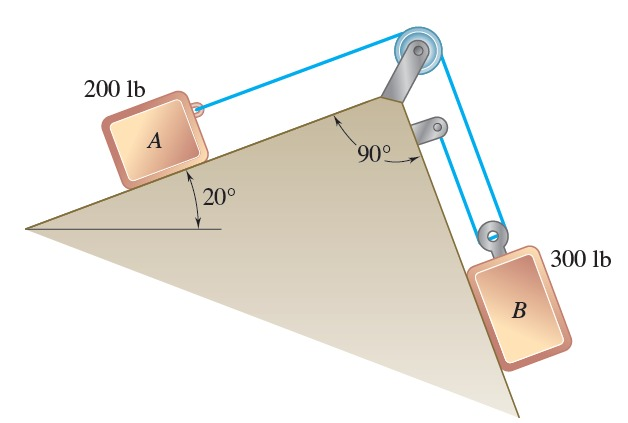
\includegraphics[width=0.75\textwidth, keepaspectratio]{4.png}
\end{center}





\item \label{qlabel:B4-Q10}
6-kg block B rests on upper surface of 10-kg block A. Neglecting friction, immediately after release: (i) acceleration of A, (ii) acceleration of B relative to A. \mk{15}
\yr{2010--11}

\begin{center}
  
\includegraphics[height=0.4\textheight,width=0.75\textwidth,keepaspectratio]{/72.png}
\end{center}




\item \label{qlabel:B4-Q13}
Two blocks originally at rest. $m_A = 50$\,kg, $m_B = 100$\,kg, $\mu_s = 0.25$, $\mu_k = 0.20$. Determine: (i) acceleration of each block, (ii) tension in cable. \mk{18}
\yr{2006--07}


\begin{center}
  
\includegraphics[width=0.75\textwidth, keepaspectratio]{/97.png}
\end{center}




\item \label{qlabel:B4-Q14}
Single wire ACB passes through ring at C attached to sphere revolving at constant speed $v$ in a horizontal circle. Mass of sphere\,$= 2.5$\,kg. Tension same in both portions. Determine speed $v$. \mk{17}
\yr{2006--07}


\begin{center}
  
\includegraphics[height=0.35\textheight,width=0.75\textwidth, keepaspectratio]{/98.png}
\end{center}





\item \label{qlabel:B4-Q15}
Block A ($m = 25$\,kg), block B ($m = 15$\,kg), $\mu_s = 0.20$, $\mu_k = 0.15$, $\theta = 25$\textdegree, $P = 250$\,N applied to A. Determine: (a) acceleration of A, (b) tension in cord. \mk{18}
\yr{2004--05}

\begin{center}
  
\includegraphics[width=0.75\textwidth, keepaspectratio]{/52.png}
\end{center}





\item \label{qlabel:B4-Q16}
20-kg block B suspended from 2-m cord attached to 30-kg cart A. Neglecting friction, immediately after release: (i) acceleration of cart, (ii) tension in cord. \mk{18}
\yr{2003--04}


\begin{center}
  
\includegraphics[width=0.75\textwidth, keepaspectratio]{/64.png}
\end{center}





\end{enumerate}

%%══════════════════════════════════════════════════════════════════════
%% SECTION B5 — Kinematics of Rigid Bodies
%%══════════════════════════════════════════════════════════════════════
\secdivider{Section B5}{Kinematics of Rigid Bodies}{cH}{cH}
\markboth{B5 --- Kinematics of Rigid Bodies}{}
\label{sec:B5}
\titleformat{\section}{\large\bfseries\color{cH}}{}{0em}{}[\titlerule]
\section{B5 --- Kinematics of Rigid Bodies}

\begin{enumerate}
\item \label{qlabel:B5-Q1}
Collar B moves downward to the left at constant velocity 1.6\,m/s. At $\theta = 40$\textdegree, determine: (a) angular velocity of rod AB, (b) velocity of collar A. \mk{15}
\yr{2023--24}

\begin{center}
  
\includegraphics[height=0.35\textheight,width=0.75\textwidth,keepaspectratio]{/122.png}
\end{center}






\item \label{qlabel:B5-Q2}
Collar B moves downward to the left at constant velocity 1.6\,m/s. At $\theta = 25$\textdegree, determine: (i) angular velocity of rod AB, (ii) velocity of collar A. \mk{15}
\yr{2023--24} \variant{B5-Q1 same setup, different angle}






\item \label{qlabel:B5-Q6}
Crank AB clockwise at 1000\,rpm, $l = 160$\,mm, $b = 60$\,mm. At $\theta = 60$\textdegree, determine velocity of piston P and angular velocity of connecting rod BD .
\mk{20}
\yr{2018--19}

\begin{center}
  
\includegraphics[height=0.4\textheight,width=0.75\textwidth,keepaspectratio]{/88.png}
\end{center}





\item \label{qlabel:B3-Q13}
A plastic film moves over two drums. During 4\,s, film speed increases uniformly from $V_0 = 1$\,m/s to $V_1 = 2$\,m/s. Determine: (i) angular acceleration of drum B, (ii) revolutions executed by drum B in 4\,s. \mk{15}
\yr{2015--16}

\begin{center}
  
\includegraphics[width=0.75\textwidth,keepaspectratio]{/35.png}
\end{center}




\item \label{qlabel:B5-Q12}
Double gear rolls on stationary left rack R. Right rack has constant velocity 2\,ft/s. Determine: (a) angular velocity of gear, (b) velocities of points A and D. Use instantaneous-centre method. \mk{15}
\yr{2014--15}


\begin{center}
  
\includegraphics[height=0.25\textheight,width=0.75\textwidth,keepaspectratio]{/107.png}
\end{center}






\item \label{qlabel:B5-Q5}
Crank AB rotates at 900\,rpm clockwise about Point $A$. Determine acceleration of piston P when $\theta = 60$\textdegree. \mk{15}
\yr{2013--14}


\begin{center}
  
\includegraphics[height=0.4\textheight,width=0.75\textwidth, keepaspectratio]{/83.png}
\end{center}




\item \label{qlabel:B5-Q3}
In an engine system, crank AB rotates clockwise at 2000\,rpm. Determine: (i) angular velocity of connecting rod BD, (ii) velocity of piston P. \mk{17}
\yr{2012--13}

\begin{center}
  
\includegraphics[height=0.3\textheight,width=0.75\textwidth, keepaspectratio]{/3.png}
\end{center}




\item \label{qlabel:B5-Q7}
Bar AB has constant angular velocity 5\,rad/s counter-clockwise. Determine angular velocities of bars BD and DE. \mk{17}
\yr{2011--12}

\begin{center}
  
\includegraphics[height=0.35\textheight,width=0.75\textwidth, keepaspectratio]{/17.png}
\end{center}





\item \label{qlabel:B5-Q8}
Bar AB has angular velocity 4\,rad/s clockwise. Determine angular velocities of bars BD and DE. \mk{20}
\yr{2010--11} \variant{B5-Q7 same linkage, different $\omega$}

\begin{center}
  
\includegraphics[height=0.4\textheight,width=0.75\textwidth,keepaspectratio]{/73.png}
\end{center}




\item \label{qlabel:B3-Q15}
A pulley starts from rest at $t=0$, accelerated at 2.4\,rad/s$^2$ clockwise. At $t=4$\,s, determine velocity and position of: (i) load A, (ii) load B. \mk{15}
\yr{2010--11}


\begin{center}
  
\includegraphics[height=0.4\textheight,width=0.75\textwidth,keepaspectratio]{/70.png}
\end{center}




\item \label{qlabel:B5-Q9}
Find angular velocity of arm DC if limb AB rotates at 2000\,rpm counter-clockwise. \mk{20}
\yr{2008--09}

\begin{center}
  
\includegraphics[width=0.75\textwidth, keepaspectratio]{/46.png}
\end{center}




\item \label{qlabel:B5-Q10}
Crank AB at 200\,rpm counter-clockwise. Determine angular velocity of rod BD and velocity of collar D when $\theta = 90$\textdegree. \mk{18}
\yr{2006--07}


\begin{center}
  
\includegraphics[height=0.3\textheight,width=0.75\textwidth, keepaspectratio]{/99.png}
\end{center}




\item \label{qlabel:B5-Q4}
Engine: $l = 200$\,mm, $b = 50$\,mm, crank AB at 2000\,rpm clockwise. At $\theta = 30$\textdegree, determine velocity of piston P and angular velocity of connecting rod. \mk{17}
\yr{2005--06}

\begin{center}
  
\includegraphics[width=0.75\textwidth, keepaspectratio]{/24.png}
\end{center}




\item \label{qlabel:B5-Q11}
Link AB rotates at 3\,rad/s clockwise. Determine angular velocities of links BC and CD at the instant shown. \mk{18}
\yr{2005--06}

\begin{center}
  
\includegraphics[height=0.35\textheight,width=0.75\textwidth, keepaspectratio]{/25.png}
\end{center}




\item \label{qlabel:B5-Q14}
Collar A moves right at constant velocity 900\,mm/s. At $\theta = 30$\textdegree, determine: (a) angular velocity of rod AB, (b) velocity of collar B. \mk{15}
\yr{2004--05}

\begin{center}
  
\includegraphics[height=0.3\textheight ,width=0.75\textwidth, keepaspectratio]{/53.png}
\end{center}




\item \label{qlabel:B5-Q15}
Derive expression for angular acceleration of rod AB in terms of $v_A$, $\theta$, $l$, and $\beta$, knowing acceleration of point B is zero. \mk{20}
\yr{2004--05}

\begin{center}
  
\includegraphics[height=0.25\textheight,width=0.75\textwidth, keepaspectratio]{/54.png}
\end{center}




\item \label{qlabel:B3-Q22}
Double pulley and two loads connected by inextensible cords. Load A: constant acceleration 2.5\,m/s$^2$ and initial velocity 3.75\,m/s, both upward. Determine: (i) revolutions executed by pulley in 3\,s, (ii) velocity and position of load B after 3\,s. \mk{18}
\yr{2003--04}

\begin{center}
  
\includegraphics[width=0.75\textwidth, keepaspectratio]{/62.png}
\end{center}




\item \label{qlabel:B3-Q23}
Velocity of collar D is 1.8\,m/s upward. Determine velocity of point A. \mk{17}
\yr{2003--04}

\begin{center}
  
\includegraphics[height=0.4\textheight,width=0.75\textwidth, keepaspectratio]{/63.png}
\end{center}







\end{enumerate}

%%══════════════════════════════════════════════════════════════════════
%% SECTION C1 — Introduction to Robotics
%%══════════════════════════════════════════════════════════════════════
\secdivider{Section C1}{Introduction to Robotics}{cA}{cA}
\markboth{C1 --- Introduction to Robotics}{}
\label{sec:C1}
\titleformat{\section}{\large\bfseries\color{cA}}{}{0em}{}[\titlerule]
\section{C1 --- Introduction to Robotics}

\begin{enumerate}
\item \label{qlabel:C1-Q2}
(a) Define joint in the context of robotics. Mention names of any four types of joints and their allowed motions. \mk{10}\\
(b) Write short notes on: (i) Robot software, (ii) Open and closed loop control systems. \mk{10}
\yr{2021--22}




%%────────────────────────────────────────────────────────────
%% C1-Q3
%%────────────────────────────────────────────────────────────
\item \label{qlabel:C1-Q1}
(a) Write short notes on: (i) Teach programming, (ii) Lead-through programming, (iii) Accuracy and repeatability of a robot. \mk{15}\\
(b) Classify grippers. Draw a schematic diagram of a common two-finger mechanical gripper. \mk{12}\\
(c) In a production chain, a manipulator drills a hole. If the next sheet is placed at twice the distance, how will a parallel manipulator react? How would a serial one react? \mk{8}
\yr{2020--21}




%%────────────────────────────────────────────────────────────
%% C1-Q2
%%────────────────────────────────────────────────────────────
\item \label{qlabel:C1-Q3}
(a) Write three robot control methods and explain each. \mk{10}\\
(b) What is the most common end-effector that provides the equivalent of a thumb and an opposing finger? \mk{5}
\yr{2019--20}




%%────────────────────────────────────────────────────────────
%% C1-Q4
%%────────────────────────────────────────────────────────────
\item \label{qlabel:C1-Q6}
(a) Define payload. Briefly classify robots according to the Japanese Industrial Robot Association (JIRA). \mk{10}\\
(b) With schematic diagram, classify and explain different types of actuators. \mk{10}
\yr{2018--19}




%%────────────────────────────────────────────────────────────
%% C1-Q7
%%────────────────────────────────────────────────────────────
\item \label{qlabel:C1-Q5}
(a) What are the specifications used to describe a robot? What are different joint drive systems used in robotics? \mk{10}\\
(b) What is a robot manipulator? How are they classified? With necessary sketch, discuss the SCARA robot arm. \mk{10}\\
(c) What is robot vision? Discuss how a robot vision system works. \mk{10}\\
(d) What do you understand by ``Degeneracy'' and ``Dexterity''? \mk{5}
\yr{2017--18}




%%────────────────────────────────────────────────────────────
%% C1-Q6
%%────────────────────────────────────────────────────────────
\item \label{qlabel:C1-Q4}
(a) What is a Robot? Mention the names and functions of robot accessories. \mk{10}\\
(b) How are robot manipulators classified? Discuss the anthropomorphic type with a suitable notation and sketch. \mk{10}
\yr{2016--17}




%%────────────────────────────────────────────────────────────
%% C1-Q5
%%────────────────────────────────────────────────────────────
\item \label{qlabel:C1-Q16}
Define payload. Briefly classify robots according to JIRA. \mk{8}
\yr{2015--16}





\item \label{qlabel:C1-Q7}
Briefly classify robots according to the Robotics Institute of America (RIA). \mk{8}
\yr{2013--14}




%%────────────────────────────────────────────────────────────
%% C1-Q8
%%────────────────────────────────────────────────────────────
\item \label{qlabel:C1-Q8}
Briefly define any two of the following: (i) Payload, (ii) Reach, (iii) Precision. \mk{6}
\yr{2013--14}




%%────────────────────────────────────────────────────────────
%% C1-Q9
%%────────────────────────────────────────────────────────────
\item \label{qlabel:C1-Q9}
What do you understand by the term ``Robot''? Define Payload, Reach, Precision, and Repeatability from the point of view of robot specification. \mk{10}
\yr{2012--13}




%%────────────────────────────────────────────────────────────
%% C1-Q10
%%────────────────────────────────────────────────────────────
\item \label{qlabel:C1-Q11}
(a) Give a brief description of the main components of a robot. \mk{10}\\
(b) What is meant by robot coordinates? With a neat sketch, explain the working space of a cylindrical coordinate robot. \mk{8}
\yr{2011--12}




%%────────────────────────────────────────────────────────────
%% C1-Q12
%%────────────────────────────────────────────────────────────
\item \label{qlabel:C1-Q10}
(a) Describe the different parameters used to depict the specification of a robot. \mk{15}\\
(b) Mention some notable applications of robots. \mk{8}
\yr{2010--11}




%%────────────────────────────────────────────────────────────
%% C1-Q11
%%────────────────────────────────────────────────────────────
\item \label{qlabel:C1-Q12}
(a) What are the steps in Machine Vision Application? \mk{5}\\
(b) Describe the types of gripper used in Industrial Robot Applications. \mk{10}
\yr{2008--09}




%%────────────────────────────────────────────────────────────
%% C1-Q13
%%────────────────────────────────────────────────────────────
\item \label{qlabel:C1-Q13}
What do you mean by cylindrical coordinate robot? Draw top and side views of workspace for this type. \mk{5}
\yr{2006--07}




%%────────────────────────────────────────────────────────────
%% C1-Q14
%%────────────────────────────────────────────────────────────
\item \label{qlabel:C1-Q14}
``One machine can do the work of a hundred ordinary men, but no machine can do the work of one extraordinary man.'' --- Discuss. \mk{5}
\yr{2004--05, 2005--06}




%%────────────────────────────────────────────────────────────
%% C1-Q15
%%────────────────────────────────────────────────────────────
\item \label{qlabel:C1-Q15}
(a) Draw the basic configurations for: (i) PPP, (ii) RRP, (iii) RYP. \mk{9}\\
(b) How do you compare end effectors and manipulator? \mk{7}\\
(c) Based on the task to be accomplished, how do you recommend the use of hydraulic vs electric drive systems? \mk{8}
\yr{2003--04}




%%────────────────────────────────────────────────────────────
%% C1-Q16
%%────────────────────────────────────────────────────────────

%% ============================================================
%%  Section C1 — Introduction to Robotics
%%  Question Bank — Answer Snippets
%%  Paste inside the C1 \begin{enumerate} ... \end{enumerate}
%% ============================================================

%%────────────────────────────────────────────────────────────
%% C1-Q1
%%────────────────────────────────────────────────────────────
\end{enumerate}

%%══════════════════════════════════════════════════════════════════════
%% SECTION C2 — Transformations & Rotation Matrices
%%══════════════════════════════════════════════════════════════════════
\secdivider{Section C2}{Plane, Rotational \& Spatial Motion; Transformations}{cB}{cB}
\markboth{C2 --- Transformations \& Rotation Matrices}{}
\label{sec:C2}
\titleformat{\section}{\large\bfseries\color{cB}}{}{0em}{}[\titlerule]
\section{C2 --- Transformations \& Rotation Matrices}

%% ══════════════════════════════════════════════════════════════════════
%% C2 — Transformations & Rotation Matrices  |  ANSWERS
%% ══════════════════════════════════════════════════════════════════════

\begin{enumerate}
\item \label{qlabel:C2-Q1}
(a) Derive a formula by which the description of a point can be changed
from one frame to another, where the frames have the same origin but
different axis orientations. \mk{10}\\
(b) Frame $\{B\}$ is rotated relative to $\{A\}$ about z-axis by
45\textdegree, then translated 2 units in $\hat{X}_A$ and 3 units in
$\hat{Y}_A$. Find ${}^AP$ if ${}^BP = [3\;7\;0]^T$. \mk{10}\\
(c) A point $P = [3\;0\;3]^T$ is subjected to: rotation about y-axis,
then translation along x-axis, then rotation about z-axis. Final
coordinates are $[4\;4\;2]^T$. Find possible transformation
variables. \mk{15}
\yr{2023--24}




%% ─────────────────────────────────────────────────────────────────────
%% C2-Q2
%% ─────────────────────────────────────────────────────────────────────
\item \label{qlabel:C2-Q2}
Frame B is rotated 90\textdegree\ about z-axis, then translated 3 and 5
units relative to n- and o-axes, then rotated 90\textdegree\ about
n-axis, then 90\textdegree\ about y-axis.\\
(i) Write the equation describing the motion.
(ii) Find new location and orientation.
\[
  B = \begin{pmatrix}
    0&1&0&1\\1&0&0&1\\0&0&{-1}&1\\0&0&0&1
  \end{pmatrix}
\]
\mk{15}
\yr{2023--24}



%% ─────────────────────────────────────────────────────────────────────
%% C2-Q3
%% ─────────────────────────────────────────────────────────────────────
\item \label{qlabel:C2-Q3}
Derive the matrix that represents a pure rotation about the y-axis of
the reference frame. \mk{10}
\yr{2016--17, 2021--22, 2023--24}




%% ─────────────────────────────────────────────────────────────────────
%% C2-Q4
%% ─────────────────────────────────────────────────────────────────────
\item \label{qlabel:C2-Q5}
(a) Derive the matrix representation of differential rotation about a
general axis $k$. \mk{10}\\
(b) Find the effect of a differential rotation of 0.1 rad about the y-axis followed by differential translation of [0.1, 0, 0.2] on the given frame B.
\[
  \text{where, } B = 
  \begin{bmatrix} 
    0 & 0 & 1 & 10 \\ 
    1 & 0 & 0 & 5 \\ 
    0 & 1 & 0 & 3 \\ 
    0 & 0 & 0 & 1 
  \end{bmatrix} 
  \quad \text{and} \quad 
  \Delta = 
  \begin{bmatrix} 
    0 & -\delta z & \delta y & dx \\ 
    \delta z & 0 & -\delta x & dy \\ 
    -\delta y & \delta x & 0 & dz \\ 
    0 & 0 & 0 & 0 
  \end{bmatrix}.
\]
\mk{10}
\yr{2017--18}




%% ─────────────────────────────────────────────────────────────────────
%% C2-Q6
%% ─────────────────────────────────────────────────────────────────────
\item \label{qlabel:C2-Q4}
In a robotic setup, a camera is attached to the fifth link of a robot with six degrees of freedom. The camera observes an object and determines its frames relative to the camera's frame. Using the following information, determine the necessary motion the end effector has to make to get to the object:
\[
  {}^5T_{cam} = \begin{bmatrix}
    0 & 0 & -1 & 3 \\
    0 & -1 & 0 & 0 \\
    -1 & 0 & 0 & 5 \\
    0 & 0 & 0 & 1
  \end{bmatrix} \qquad
  {}^5T_H = \begin{bmatrix}
    0 & -1 & 0 & 0 \\
    1 & 0 & 0 & 0 \\
    0 & 0 & 1 & 4 \\
    0 & 0 & 0 & 1
  \end{bmatrix}
\]
\[
  {}^{cam}T_{obj} = \begin{bmatrix}
    0 & 0 & 1 & 2 \\
    1 & 0 & 0 & 2 \\
    0 & 1 & 0 & 4 \\
    0 & 0 & 0 & 1
  \end{bmatrix} \qquad
  {}^HT_E = \begin{bmatrix}
    1 & 0 & 0 & 0 \\
    0 & 1 & 0 & 0 \\
    0 & 0 & 1 & 3 \\
    0 & 0 & 0 & 1
  \end{bmatrix}
\]




%% ─────────────────────────────────────────────────────────────────────
%% C2-Q5
%% ─────────────────────────────────────────────────────────────────────
\item \label{qlabel:C2-Q7}
Derive the matrix that represents a pure rotation about the x-axis of
the reference frame. \mk{15}
\yr{2014--15}




%% ─────────────────────────────────────────────────────────────────────
%% C2-Q8
%% ─────────────────────────────────────────────────────────────────────
\item \label{qlabel:C2-Q6}
Prove that a rotation matrix is a unitary matrix. \mk{12}
\yr{2013--14}




%% ─────────────────────────────────────────────────────────────────────
%% C2-Q7
%% ─────────────────────────────────────────────────────────────────────
\item \label{qlabel:C2-Q8}
(a) Derive the relation $\bar{P}_{xyz} = \bar{R}\,\bar{P}_{uvw}$ and
find $\bar{R}$ if OUVW is rotated by angle $\phi$ about OY. \mk{10}\\
(b) A point is subjected to: (i) translation 5 units along $+Y$,
(ii) CW rotation 30\textdegree\ about OX, (iii) CCW rotation
30\textdegree\ about OZ, (iv) translation 3 units along $-X$. Write
the combined transformation equation. \mk{10}
\yr{2006--07}




%% ─────────────────────────────────────────────────────────────────────
%% C2-Q9
%% ─────────────────────────────────────────────────────────────────────
\item \label{qlabel:C2-Q10}
(a) Derive the relation $P_{uvw} = Q\,P_{xyz}$. \mk{7}\\
(b) Write down the mathematical relation between OXYZ and OUVW for the
following motion sequence: (i) CW rotation $\alpha$ about OX, (ii) CW
rotation $\beta$ about OZ, (iii) CCW rotation $\alpha$ about rotated
Ou, (iv) CCW rotation $\beta$ about rotated OV, (v) CCW rotation
$\alpha$ about OY, (vi) translation $d_y$ along OY, (vii) CW rotation
$\alpha$ about rotated OW, (viii) translation $d_x$ along negative
OX. \mk{20}
\yr{2004--05}




%% ─────────────────────────────────────────────────────────────────────
%% C2-Q11
%% ─────────────────────────────────────────────────────────────────────
\item \label{qlabel:C2-Q11}
Determine $P_{xyz}$ given:
$P_{xyz} = [R_{z,45\textdegree}\;R_{y,-30\textdegree}\;T_{z,5}]\,P_{uvw}$,
where $P_{uvw}$ is given. \mk{8}
\yr{2004--05}




\item \label{qlabel:C2-Q9}
(a) Derive the rotation matrix $R$ transforming coordinates from
$P_{uvw}$ to $P_{xyz}$. Hence find homogeneous transformation matrix $T$
representing: CW rotation $\alpha$ about OX, then CCW rotation $\theta$
about OZ, then CW rotation $\phi$ about OY. \mk{25}\\
(b) Given $Q_{uvw} = (4,3,2)^T$, determine corresponding point after:
CCW rotation 45\textdegree\ about OX, then translation 5 units along
OZ. \mk{10}
\yr{2003--04}




%% ─────────────────────────────────────────────────────────────────────
%% C2-Q10
%% ─────────────────────────────────────────────────────────────────────

%% ─────────────────────────────────────────────────────────────────────
%% C2-Q1
%% ─────────────────────────────────────────────────────────────────────
\end{enumerate}
%%══════════════════════════════════════════════════════════════════════
%% SECTION C3 — Configurations & Workspace
%%══════════════════════════════════════════════════════════════════════
\secdivider{Section C3}{Geometric Configurations: Linkages, Arms, Workspace}{cC}{cC}
\markboth{C3 --- Configurations \& Workspace}{}
\label{sec:C3}
\titleformat{\section}{\large\bfseries\color{cC}}{}{0em}{}[\titlerule]
\section{C3 --- Geometric Configurations \& Workspace}

\begin{enumerate}
\item \label{qlabel:C3-Q1}
(a) Sketch the following manipulator configurations: (i) TR:TLO, (ii) TR:TR. For each, determine the workspace of the wrist portion. \mk{10}\\
(b) Desired to place origin of hand frame of a cylindrical robot at $p = [-3\;4\;7]^T$. Calculate the joint variables. \mk{10}
\yr{2023--24}




%%────────────────────────────────────────────────────────────────────
%% C3-Q2
%%────────────────────────────────────────────────────────────────────

\item \label{qlabel:C3-Q2}
A cylindrical robot has three DOF: move along x-axis, rotate about z-axis, move along z-axis. Determine the $4\times4$ transformation matrix and hence find joint variables to place hand frame origin at $[6,\;-3,\;-4]^T$. \mk{15}
\yr{2021--22} \variant{C3-Q1 same concept, different target}





%%────────────────────────────────────────────────────────────────────
%% C3-Q3
%%────────────────────────────────────────────────────────────────────
\item \label{qlabel:C3-Q3}
Briefly classify robots according to various robot coordinates. Derive
the single matrix $T_{\mathrm{cyl}}(r,\alpha,l)$ for the cylindrical
coordinate system. \mk{12}
\yr{2015--16, 2021--22}




%%────────────────────────────────────────────────────────────────────
%% C3-Q4
%%────────────────────────────────────────────────────────────────────
\item \label{qlabel:C3-Q4}
Cylindrical robot transformation:
$T_{\mathrm{cyl}}(r,\alpha,l) = \mathrm{Trans}(0,0,l)\;\mathrm{Rot}(z,\alpha)\;\mathrm{Trans}(r,0,0)$.
Arm then rotated at $-\alpha$ about z-axis.\\
(i) Derive the necessary matrix. (ii) If desired to place hand frame
origin at $T$, calculate joint variables. \mk{10+5}
\yr{2017--18}




%%────────────────────────────────────────────────────────────────────
%% C3-Q6 — SKIP (image-based workspace diagram)
%%────────────────────────────────────────────────────────────────────
\item \label{qlabel:C3-Q6}
The robotic manipulator is a spherical robot (two revolute + one prismatic joint). Restrictions: Link 1: $0 \leq$ Rotation about OZ $\leq 120$\textdegree; Link 2: $0 \leq$ Rotation about O$'$Y$' \leq 60$\textdegree; Link 3: Translation along X$'$. Draw top and side views of work volume. \mk{8}
\yr{2005--06}

\begin{center}
  
\includegraphics[height=0.3\textheight,width=0.75\textwidth, keepaspectratio]{/26.png}
\end{center}

% [Answer involves workspace sketch — see diagram in question paper]

%%────────────────────────────────────────────────────────────────────
%% C3-Q7
%%────────────────────────────────────────────────────────────────────
\item \label{qlabel:C3-Q7}
(a) While setting chips and designing circuitry onto a motherboard,
what essential factors should an end effector take into
consideration? \mk{6}\\
(b) Is it possible to use an AC power supply for a mobile robot
designed to follow a predefined path? Discuss. \mk{6}
\yr{2004--05}




%%────────────────────────────────────────────────────────────────────
%% C3-Q8 — SKIP (image-based workspace diagram)
%%────────────────────────────────────────────────────────────────────

\item \label{qlabel:C3-Q8}
Draw the schematic diagram of the work volume for a robotic configuration with the following restrictions:\\
Link 1: translation along Y-axis $= d_y$;\\
Link 2: translation along length $= d_L$; $0 \leq$ Rotation about Y $\leq 120$\textdegree;\\
Link 3: $0 \geq$ Rotation about O$''$Z$'' \geq -45$\textdegree;\\
Link 4: $0 \leq$ Rotation about O$''$Z$'' \leq 45$\textdegree. \mk{18}
\yr{2004--05}

\begin{center}
  
\includegraphics[width=0.75\textwidth, keepaspectratio]{/55.png}
\end{center}
% [Answer involves workspace sketch — see diagram in question paper]



%%────────────────────────────────────────────────────────────────────
%% C3-Q1
%%────────────────────────────────────────────────────────────────────
\end{enumerate}

%%══════════════════════════════════════════════════════════════════════
%% SECTION C4 — Motion Characteristics & Applied Transformations
%%══════════════════════════════════════════════════════════════════════
\secdivider{Section C4}{Motion Characteristics}{cD}{cD}
\markboth{C4 --- Motion Characteristics}{}
\label{sec:C4}
\titleformat{\section}{\large\bfseries\color{cD}}{}{0em}{}[\titlerule]
\section{C4 --- Motion Characteristics}

\begin{enumerate}
\item \label{qlabel:C4-Q7}
Point $P(3,0,3)^T$ subjected to: rotation about y-axis, then
translation along x-axis, then rotation about z-axis. Final coordinates
are $[4\;4\;2]^T$. Find possible transformation variables. \mk{15}
\yr{2023--24}
\variant{C2-Q1(c) — identical problem}




%%────────────────────────────────────────────────────────────────────
%% C4-Q8 — SKIP (image-based workspace diagram)
%%────────────────────────────────────────────────────────────────────
\item \label{qlabel:C4-Q5}
Point $P(7,3,2)^T$ subjected to: (i) rotation 90\textdegree\ about
z-axis, (ii) translation $[4,-3,7]$, (iii) rotation 90\textdegree\
about y-axis. Find final coordinates. \mk{15}
\yr{2018--19}




%%────────────────────────────────────────────────────────────────────
%% C4-Q6
%%────────────────────────────────────────────────────────────────────
\item \label{qlabel:C4-Q4}
Point $P(6,8,5)^T$ subjected to: (i) translation $[2,-3,7]$,
(ii) rotation 30\textdegree\ about x-axis, (iii) translation
$[-1,4,3]$. Find coordinates. \mk{15}
\yr{2015--16}




%%────────────────────────────────────────────────────────────────────
%% C4-Q5
%%────────────────────────────────────────────────────────────────────
\item \label{qlabel:C4-Q3}
Point $P(5,4,7)^T$ subjected to: (i) rotation 90\textdegree\ about
z-axis, (ii) translation $[4,-3,2]$, (iii) rotation 45\textdegree\
about y-axis. Find final coordinates. \mk{20}
\yr{2014--15}




%%────────────────────────────────────────────────────────────────────
%% C4-Q4
%%────────────────────────────────────────────────────────────────────
\item \label{qlabel:C4-Q2}
Point $P(4,5,3)^T$ subjected to: (i) rotation 90\textdegree\ about
z-axis, (ii) translation $[3,-2,1]$. Find coordinates relative to
reference frame. \mk{15}
\yr{2013--14}




%%────────────────────────────────────────────────────────────────────
%% C4-Q3
%%────────────────────────────────────────────────────────────────────
\item \label{qlabel:C4-Q1}
A point $T$ is attached to frame $(n,o,a)$ initially aligned with
global frame $(x,y,z)$. Subjected to: (i) rotation $+30\textdegree$ about
x-axis, (ii) rotation $-90\textdegree$ about a-axis, (iii) translation
$[0,\;4\sqrt{3},\;-2\sqrt{3}]$ along $(x,y,z)$. Find new
coordinates. \mk{25}
\yr{2012--13}




%%────────────────────────────────────────────────────────────────────
%% C4-Q2
%%────────────────────────────────────────────────────────────────────
\item \label{qlabel:C4-Q6}
Point $P(3,3,0)^T$ subjected to: (i) CW rotation 45\textdegree\ about
Y, (ii) CCW rotation 45\textdegree\ about X, (iii) translation
$[C,\;2,\;2]$. Find coordinates relative to OXYZ. \mk{20}
\yr{2005--06}




%%────────────────────────────────────────────────────────────────────
%% C4-Q7  (same as C2-Q1(c))
%%────────────────────────────────────────────────────────────────────
\item \label{qlabel:C4-Q8}
(a) Define work envelope. Draw schematic of work envelope for a robot
with the given link restrictions. \mk{11}
\yr{2003--04}


\begin{center}
  
\includegraphics[height=0.25\textheight,width=0.75\textwidth, keepaspectratio]{/65.png}
\end{center}

% [Answer involves workspace sketch — see diagram in question paper]


%%────────────────────────────────────────────────────────────────────
%% C4-Q1
%%────────────────────────────────────────────────────────────────────
\end{enumerate}

\end{document}